\documentclass[pdflatex,11pt]{aghdpl}

%\documentclass{aghdpl}               % przy kompilacji programem latex
%\documentclass[pdflatex,en]{aghdpl}  % praca w j�zyku angielskim
%\usepackage[polish]{babel}
%\usepackage[latin2]{inputenc}

%\usepackage[english]{babel}
\usepackage[english, polish]{babel}
\usepackage[utf8]{inputenc}
%\usepackage[cp1250]{inputenc}

% wzory w jednym wierszu obok siebie i tekst mi�dzy nimi
\usepackage{amsmath}

% rysunki a, b, c ...
\usepackage{subfig}

% umieszczanie rysunk�w dok�adnie w miejscu wstawienia (H)
\usepackage{float}

% indeks dolny 
\usepackage{fixltx2e}

\usepackage{longtable}

\usepackage{graphicx, array, blindtext}
\usepackage[export]{adjustbox}

% rozmiar czcionki w opisach rysunk�w
\usepackage[font=footnotesize,labelfont=bf]{caption}
%   scriptsize
%   footnotesize
%   small
%   normalsize
%   large
%   Large

% opis tabeli nad tabel�
\usepackage{float}

\floatstyle{plaintop}
\restylefloat{table}

% wy��czenie dzielenia wyraz�w na ko�cu linii
\usepackage[none]{hyphenat}

% pogrubienie linii w tabelach
\usepackage{booktabs}

% wielowierszowe r�wnania (\begin{aligned} \end{aligned} wewn�trz {equation}, znak wyr�wnania "`&"'
\usepackage{amsmath}

% dodatkowe pakiety
%\usepackage{enumerate}
\usepackage{enumitem}
\usepackage{listings}

% wielowierszowe kom�rki w tabelach
\usepackage{multirow}

\usepackage{array}

%\usepackage{natbib}
%\usepackage{multibib}
%\newcites{misc}{Miscellaneous}	% https://tex.stackexchange.com/questions/93845/suppress-printing-of-only-bibentry-references-with-natbib
\usepackage{bibentry}
\nobibliography*

% cudzys��w w tytyle w bibliografii
\usepackage{csquotes}

% dodaj pliki pfg
\usepackage{pdfpages} 

\usepackage{textcomp}

% kolorowe hiperlinki
\usepackage{xcolor}

\usepackage[
hidelinks,	% ukrycie prostok�nych obw�dek hiperlink�w
linktocpage,	% ustawienie w toc, lof i lot, �e tylko numer strony jest hiperlinkiem
ocgcolorlinks,	% czarne hiperlinki w wydruku
bookmarks,
bookmarksopen,
bookmarksopenlevel=2,
bookmarksnumbered,
pdfstartview=Fit,
%pdfview=FitH
]{hyperref}

\hypersetup{
	pdftitle={Low-loss microwave circuits in strip transmission line technique},
	pdfauthor={Jakub Sorocki}
}

% kolory hiperlink�w
\hypersetup{	
    colorlinks,
    linkcolor={red!55!black},
    citecolor={blue!55!black},
    urlcolor={blue!80!black}
}

\lstloadlanguages{TeX}

%---------------------------------------------------------------------------

\author{Piotr Rzeszut}
\shortauthor{P. Rzeszut}

\titlePL{Statyczna i dynamiczna charakteryzacja magnetycznych z\l{}\c acz tunelowych z anizotropi\c a prostopad\l{}\c a.}
\titleEN{Static and dynamic characterization of magnetic tunnel junctions with perpendicular anisotropy.}

\shorttitlePL{Statyczna i dynamiczna charakteryzacja magnetycznych z\l{}\c acz tunelowych....} % skr�cona wersja tytu�u je�li jest bardzo d�ugi
\shorttitleEN{Static and dynamic characterization of magnetic tunnel junctions...}

\thesistypePL{Rozprawa doktorska}
\thesistypeEN{Ph.D. Thesis}

\supervisorPL{dr hab. inz. Witold Skowroński, prof. n. AGH}
\supervisorEN{Prof. Witold Skowroński, D.Sc.}

\date{2022}
\dateMonth{June}

\departmentPL{Instytut Elektroniki}
\departmentEN{Institute of Electronics}

\facultyPL{Wydzia\l{} Informatyki, Elektroniki i Telekomunikacji}
\facultyEN{Faculty of Computer Science, Electronics and Telecommunications}

\setlength{\cftsecnumwidth}{10mm}

%---------------------------------------------------------------------------

\begin{document}


%--- front matter --
% dedication, declaration, acknowledgement, abstract
% title page, author, copyright, abstract, streszczenie, acknowledgements, list of papers
\titlepages
 
% tableofcontents, list of figures, list of tables, nomenclature

\fancyhead[LO]{\slshape{\small Contents}}
\fancyhead[RO]{\bfseries \thepage}
\fancyhead[RE]{\slshape{\small Contents}}
\fancyhead[LE]{\bfseries \thepage}

\tableofcontents
\cleardoublepage 

\fancyhead[LO]{\slshape{\small List of Papers}}
\fancyhead[RO]{\bfseries \thepage}
\fancyhead[RE]{\slshape{\small List of Papers}}
\fancyhead[LE]{\bfseries \thepage}
\chapter*{List of papers}\label{papers}
\addcontentsline{toc}{chapter}{List of papers}	% to be visible in TOC but unnuvered

\noindent This Thesis is based on and incorporates the following publications:\\

\noindent Chapter \hyperref[lhrh]{3}:\\% Chapter 3 - Application of novel realization schemes and constitutive elements topologies to improve performance and minimize power loss
\noindent - \bibentry{rzeszut2019multi}.\\

\noindent Chapter \hyperref[performance]{4}:\\% Chapter 4 - Circuits` topology optimization focused on the performance improvement and functionalities integration as a way of power loss reduction
\noindent - \bibentry{isap_miniaturized_DF}.\\
\noindent - \bibentry{mwcl_band_reject}.\\
\noindent - \bibentry{tmtt_crosscoupled_DF}.\\
\noindent - \bibentry{mikon_cascaded_DF}.\\
\noindent - \bibentry{mwcl_cascaded_multipex}.\\
\noindent - \bibentry{jmwt_imp_tranforming}.\\
\noindent - \bibentry{mwcl_tandem}.\\
%\noindent - \bibentry{jiee_imp_tranf_balun}\\

\noindent Chapter \hyperref[emerging]{5}:\\% Chapter 5 - Introduction of emerging materials and manufacturing technologies for low-loss circuits realization
\noindent - \bibentry{iceese_3D_graphene}.\\
\noindent - \bibentry{ectc_electrify}.\\
\noindent - \bibentry{ectc_df}.\\
\noindent - \bibentry{polyjet_susp_coupler}.\\

\noindent Chapter \hyperref[front]{6} :\\% Chapter 6 - stroik i wzmacniacz
\noindent - \bibentry{rws_imp_tuner}.\\
%\noindent - \bibentry{avionix_report}\\

\cleardoublepage

%\fancyhead[LO]{\slshape{\small List of Figures}}
%\fancyhead[RO]{\bfseries \thepage}
%\fancyhead[RE]{\slshape{\small List of Figures}}
%\fancyhead[LE]{\bfseries \thepage}
%
%\listoffigures
%\cleardoublepage

%\fancyhead[LO]{\slshape{\small List of Tables}}
%\fancyhead[RO]{\bfseries \thepage}
%\fancyhead[RE]{\slshape{\small List of Tables}}
%\fancyhead[LE]{\bfseries \thepage}
%
%\listoftables
%\cleardoublepage

%\fancyhead[LO]{\slshape{\small List of Abbreviations}}
%\fancyhead[RO]{\bfseries \thepage}
%\fancyhead[RE]{\slshape{\small List of Abbreviations}}
%\fancyhead[LE]{\bfseries \thepage}
%
%\printnomenclature
%\cleardoublepage

%--- main paper ---

\fancyhead[LO]{\slshape{\small \rightmark}}
\fancyhead[RO]{\bfseries \thepage}
\fancyhead[RE]{\slshape{\small \leftmark}}
\fancyhead[LE]{\bfseries \thepage}

\chapter{Introduction}\label{intro}

\section{Significance of the research}\label{intro:impact}

\indent Spin electronics 


\section{Scientific goals and organization of the Thesis}\label{intro:goal}

This Thesis presents a comprehensive study of 


\cleardoublepage
\chapter{Strip transmission line medium for TEM wave propagation}\label{theory}

\indent The development of waveguide and other transmission lines for the low-loss power transmission at high frequencies was one of the early milestones in microwave engineering. Transmission in early RF and microwave systems relied on waveguides, two-wire lines, and coaxial lines. Waveguides have the advantage of high power-handling capability and low loss, but are bulky and expensive, especially at low frequencies. Two-wire lines are inexpensive, but lack shielding. Coaxial lines are shielded but are a difficult medium to fabricate complex microwave components. Planar transmission lines provide an alternative, in the form of stripline, microstrip lines, slotlines, coplanar waveguides, and several other types of related geometries. Such transmission lines are compact, low in cost, and capable of being easily integrated with active circuit devices, such as diodes and transistors, to form microwave integrated circuits.
\\
\indent In this chapter a transmission line that consist of two or more conductors and support transverse electromagnetic (TEM) waves is considered. A transmission line can be characterized by the propagation constant, the attenuation constant, and the characteristic impedance \cite{balanis} which are derived here to provide theoretical background for further analysis.
\\
\indent Even though, transmission lines are lossy structures due to finite conductivity and/or lossy dielectric, these losses are usually small and for many practical problems may be neglected. However, when e.g. high power circuits with low line attenuation are necessary, resonant circuits in which very high quality factor are of need or low-noise feeding networks for active circuits are required, the effect of loss must be taken into account. Therefore, a lossy transmission line is considered here to allow for inclusion of the loss effects on a transmission line behavior \cite{pozar}.


\section{Wave propagation in a lossy transmission line}\label{th:lossy}

\indent A one dimensional section of transmission line shown schematically in Fig. \ref{th:fig1a} as a two-wire line representation can be considered in terms of propagating voltage and current waves along $z$-axis. At a distance $z$, there is current $I(z)$ traveling through each wire, and there is voltage difference $V(z)$ between the wires. To calculate their distance and time relations, a transmission line model shown in Fig. \ref{th:fig1b} can be used. The section of line of infinitesimal length $\Delta z$ is modeled as a lumped-element circuit, where $L$, $R$, $C$, $G$, are per-unit-length quantities defined as follows:

\begin{itemize}[nosep]
\item $L$ is a series inductance per unit length, for both conductors, in (H/m), representing the total self-inductance of two conductors;
\item $R$ is a series resistance per unit length, for both conductors, in ($\Omega$/m), representing the resistance due to the finite conductivity of the individual conductors;
\item $C$ is a shunt capacitance per unit length, in (F/m), representing the total self-capacitance due to the close proximity of the two conductors;
\item $G$ is a shunt conductance per unit length, in (S/m), representing the dielectric loss in the material between the conductors.
\end{itemize}

\noindent A finite length of a transmission line can be seen as a cascade of sections of the form shown in Fig. \ref{th:fig1b}. 

%%%%%%%%%%%%%%%%%%%%%%%%%%%%%%%%%%%%%%%%%%%%%%%%%%%%%%%%%%%%%
\begin{figure}[H]
\centering
\begin{tabular}{c}
\subfloat[] { 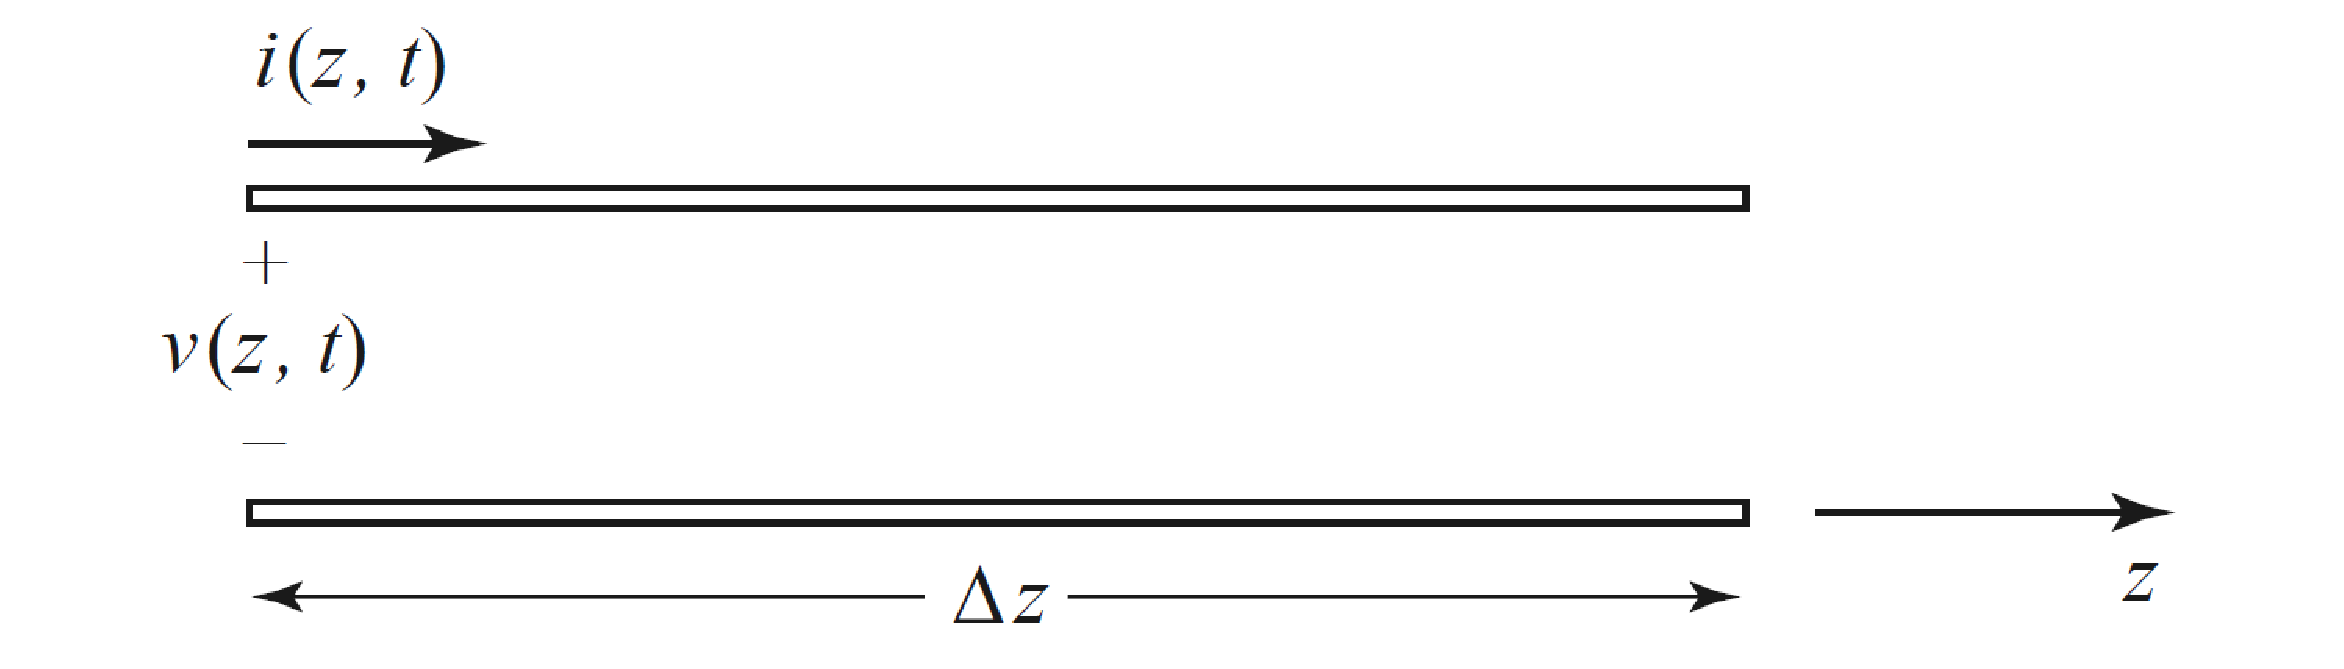
\includegraphics[scale=0.25]{chapter_2/fig1a.eps}\label{th:fig1a} }
\\
\subfloat[] { 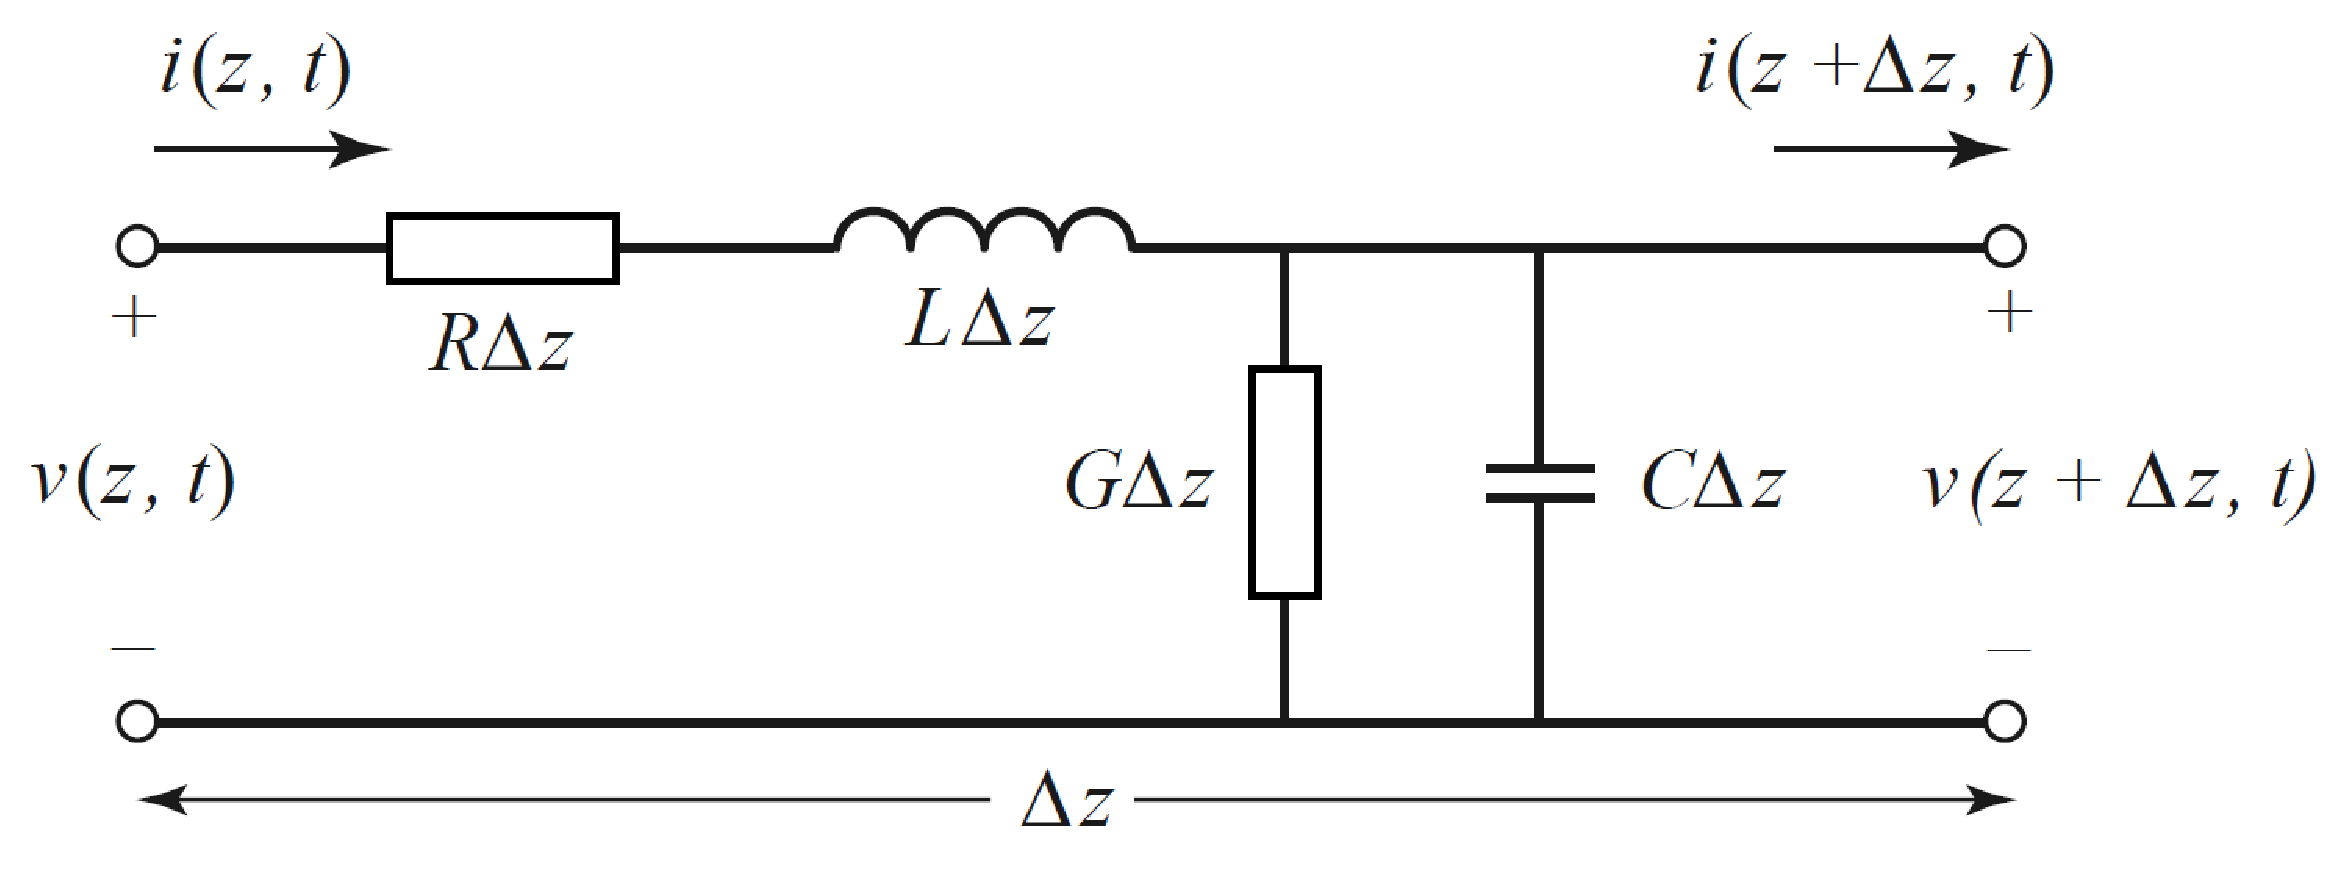
\includegraphics[scale=0.25]{chapter_2/fig1b.eps}\label{th:fig1b} }
\\
\end{tabular}
\caption{Definitions of voltage and current (a) together with lumped-element equivalent circuit for an incremental length of transmission line (b)}
\label{th:fig1}
\end{figure}
%%%%%%%%%%%%%%%%%%%%%%%%%%%%%%%%%%%%%%%%%%%%%%%%%%%%%%%%%%%%%

\indent From the circuit shown in Fig. \ref{th:fig1b}, Kirchhoff’s voltage law can be applied to give:

\begin{subequations}
\begin{equation}\label{th:eq1a}
v(z,t)-R\Delta zi(z,t)-L\Delta z\frac{\partial i(z,t)}{\partial t}-v(z+\Delta z,t)=0,
\end{equation}
and Kirchhoff’s current law leads to:
\begin{equation}\label{th:eq1b}
i(z,t)-G\Delta zv(z+\Delta z,t)-C\Delta z\frac{\partial v(z+\Delta z,t)}{\partial t}-i(z+\Delta z,t)=0.
\end{equation}
\end{subequations}

\noindent Dividing \ref{th:eq1a} and \ref{th:eq1b} by $\Delta z$ and taking the limit as $\Delta z \rightarrow 0$ gives the following differential equations:

\begin{subequations}
\begin{equation}\label{th:eq2a}
\frac{\partial v(z,t)}{\partial z}=-Ri(z,t)-L\frac{\partial i(z,t)}{\partial t},
\end{equation}
\begin{equation}\label{th:eq2b}
\frac{\partial i(z,t)}{\partial z}=-Gv(z,t)-C\frac{\partial v(z,t)}{\partial t}.
\end{equation}
\end{subequations}

\noindent These are the time domain form of the transmission line equations, also known as the telegrapher equations.
\\
\indent For the sinusoidal steady-state condition, with cosine-based phasors, \ref{th:eq2a} and \ref{th:eq2b} simplify to:

\begin{subequations}\label{th:eq3} 
\begin{equation}\label{th:eq3a}
\frac{dV(z)}{dz}=-(R+j\omega L)I(z),
\end{equation}
\begin{equation}\label{th:eq3b}
\frac{dI(z)}{dz}=-(G+j\omega C)V(z).
\end{equation}
\end{subequations}

\indent Following, the two equations \ref{th:eq3a} and \ref{th:eq3b} can be solved simultaneously to give wave equations for $V(z)$ and $I(z)$:

\begin{subequations}\label{th:eq4}
\begin{equation}\label{th:eq4a}
\frac{d^{2}V(z)}{dz^{2}}-\gamma ^{2}V(z)=0,
\end{equation}
\begin{equation}\label{th:eq4b}
\frac{d^{2}I(z)}{dz^{2}}-\gamma ^{2}I(z)=0,
\end{equation}
\end{subequations}

\begin{equation}\label{th:eq5}
\gamma = \alpha + j\beta = \sqrt{(R+j\omega L)(G+j\omega C)}
\end{equation}

\noindent where \ref{th:eq5} is the complex propagation constant, which is a function of frequency. Traveling wave solutions to \ref{th:eq4} can be found as:

\begin{subequations}\label{th:eq6}
\begin{equation}\label{th:eq6a}
V(z)=V_{o}^{+}e^{-\gamma z}+V_{o}^{-}e^{\gamma z},
\end{equation}
\begin{equation}\label{th:eq6b}
I(z)=I_{o}^{+}e^{-\gamma z}+I_{o}^{-}e^{\gamma z},
\end{equation}
\end{subequations}

\noindent where the $e^{-\gamma z}$ term represents wave propagation in the $+z$ direction, and the $e^{\gamma z}$ term represents wave propagation in the $-z$ direction. Applying \ref{th:eq3a} to the voltage of \ref{th:eq6a} gives the current on the line:

\begin{equation}\label{th:eq7}
I(z)=\frac{\gamma}{R+j\omega L}(V_{o}^{+}e^{-\gamma z}+V_{o}^{-}e^{\gamma z}).
\end{equation}

\indent Comparison of \ref{th:eq7} with \ref{th:eq6b} shows that the characteristic impedance $Z_{0}$, can be defined as:

\begin{equation}\label{th:eq8}
Z_{0}=\frac{R+j\omega L}{\gamma}=\sqrt{\frac{R+j\omega L}{G+j\omega C}},
\end{equation}

\noindent to relate the voltage and current on the line as follows:

\begin{equation}\label{th:eq9}
\frac{V_{o}^{+}}{I_{o}^{+}}=Z_{0}=\frac{-V_{o}^{-}}{I_{o}^{-}}.
\end{equation}

\noindent Then \ref{th:eq6b} can be rewritten in the following form:

\begin{equation}\label{th:eq10}
I(z)=\frac{V_{o}^{+}}{Z_{0}}e^{-\gamma z}-\frac{V_{o}^{-}}{Z_{0}}e^{\gamma z}.
\end{equation}

\indent Converting back to the time domain, we can express the voltage waveform as:

\begin{equation}\label{th:eq11}
v(z,t)=|V_{o}^{+}|cos(\omega t-\beta z +\phi ^{+})e^{-\alpha z}+|V_{o}^{-}|cos(\omega t+\beta z +\phi ^{-})e^{\alpha z},
\end{equation}

\noindent where $\phi ^{\pm }$ is the phase angle of the complex voltage $V_{o}^{\pm }$. Moreover, the wavelength on the line is

\begin{equation}\label{th:eq12}
\lambda = \frac{2\pi }{\beta },
\end{equation}

\noindent while the phase and group velocities are

\begin{subequations}\label{th:eq13}
\begin{equation}\label{th:eq13a}
v_{p} = \frac{\omega }{\beta }=\lambda f=\frac{1}{\sqrt{\epsilon \mu }},
\end{equation}
\begin{equation}\label{th:eq13b}
v_{g} = \frac{\partial \omega }{\partial \beta }.
\end{equation}
\end{subequations}

\indent The phase velocity $v_p$ corresponds to the propagation of a perturbation, i.e. it is the velocity at which a fixed phase point on the wave travels, while the group velocity $v_g$ corresponds to the propagation of energy. In a conventional medium, where permittivity $\epsilon $ and permability $\mu $ are greater than 0, the Electric field–Magnetic field–propagation constant ($\overline{E},\overline{H},\overline{\beta }$) builds the right-handed (RH) triad, therefore $v_p$ and $v_g$ are positive values describing a forward-wave propagation, outward from the source. However, if a medium would feature $\epsilon ,\mu$ < 0, a left-handed (LH) triad is build \cite{caloz}. Thus, as frequency is always a positive quantity, the phase velocity in a LH medium would be opposite to the phase velocity in a RH medium. Moreover, because $\beta $ is known to be positive in a RH medium, it would be negative in a LH medium, hence phase as related to the phase velocity, propagates backwards to the source in the opposite direction than that of power as being related to the group velocity.

\section{Power loss in a terminated lossy transmission line}\label{th:terminated}
%\section{Attenuation constant on a terminated lossy transmission line}\label{th:terminated}

The voltage and current wave propagating along a length $l$ of a lossy transmission line terminated by the impedance $Z_{L}$, as shown in Fig. \ref{th:fig2}, with propagation constant $\beta $ is attenuated at a constant rate of $\alpha $. Thus, $\gamma = \alpha + j\beta $ is complex, however, it is assumed that loss is small, so that $Z_{0}$ is approximately real. The actual power delivered to the load can be determined using the analysis given below.

%%%%%%%%%%%%%%%%%%%%%%%%%%%%%%%%%%%%%%%%%%%%%%%%%%%%%%%%%%%%%
\begin{figure}[H]
\centering
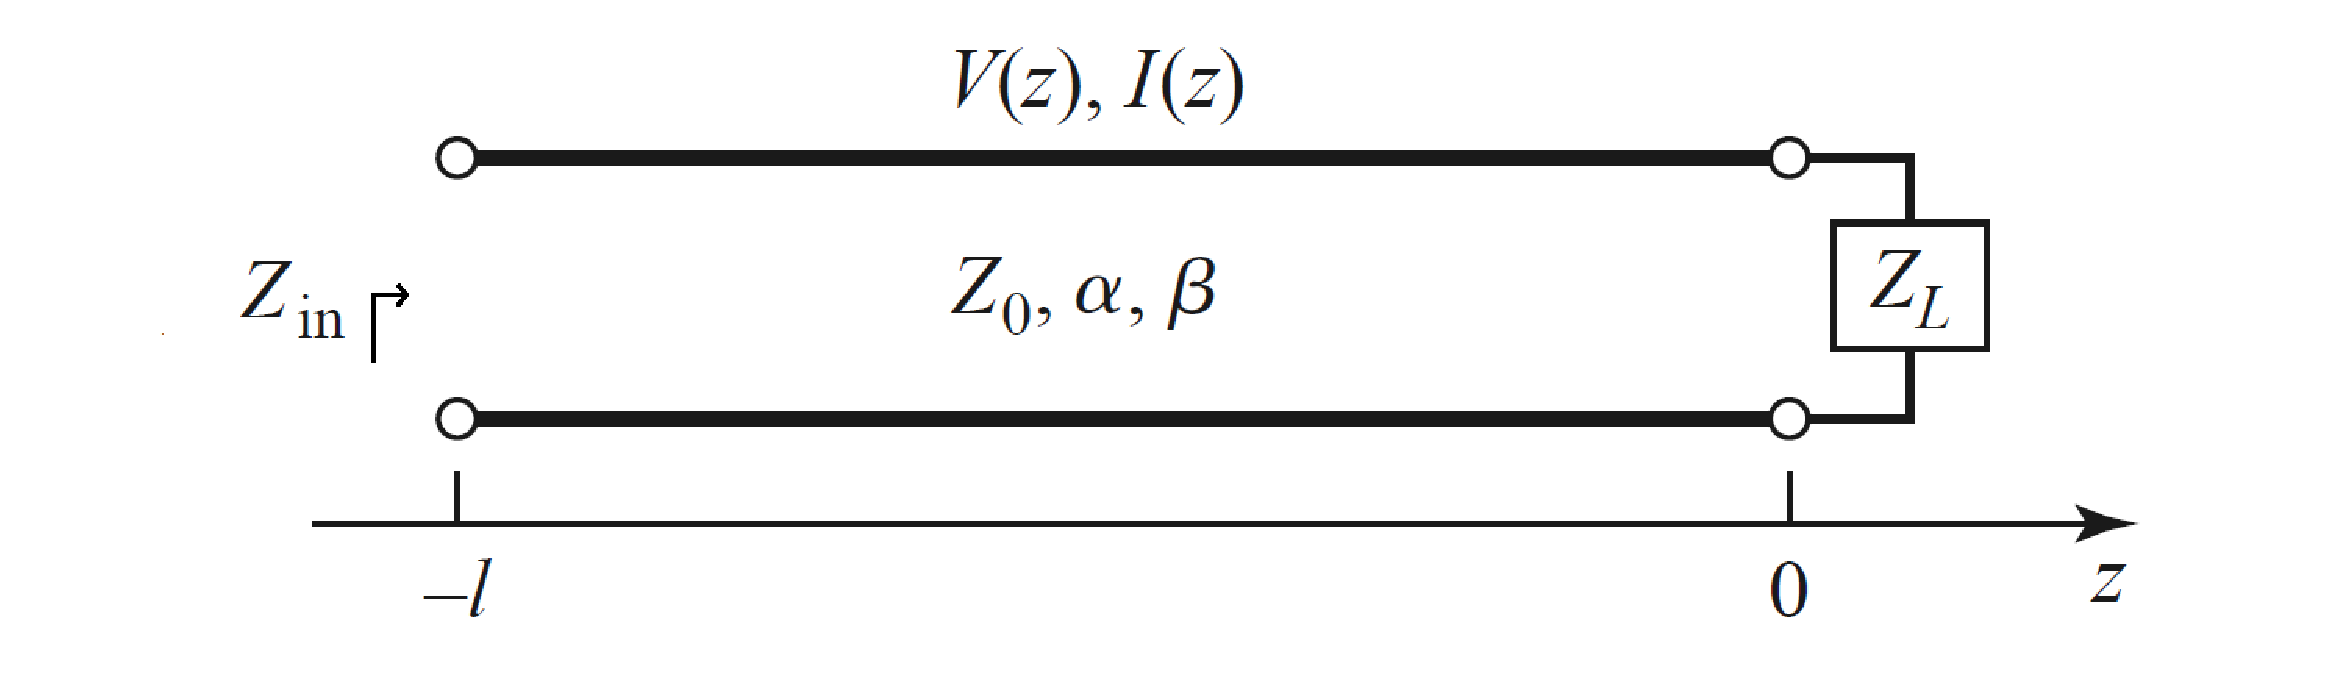
\includegraphics[scale=0.25]{chapter_2/fig2.eps}
\caption{A lossy transmission line terminated by the impedance $Z_{L}$.}
\label{th:fig2}
\end{figure}
%%%%%%%%%%%%%%%%%%%%%%%%%%%%%%%%%%%%%%%%%%%%%%%%%%%%%%%%%%%%%

\indent The voltage and current wave can be expressed as:

\begin{subequations}\label{th:eq14}
\begin{equation}\label{th:eq14a}
V(z)=V_{o}^{+}(e^{-\gamma z}+\Gamma e^{\gamma z}),
\end{equation}
\begin{equation}\label{th:eq14b}
I(z)=\frac{V_{o}^{+}}{Z_{0}}(e^{-\gamma z}-\Gamma e^{\gamma z}),
\end{equation}
\end{subequations}

\noindent where $\Gamma $ is the reflection coefficient of the load and $V_{o}^{+}$ is the incident
voltage amplitude referenced at $z$ = 0. The reflection coefficient at a distance $l$ from the load is:

\begin{equation}\label{th:eq15}
\Gamma (l)=\Gamma e^{-2j\beta l}e^{-2\alpha l}=\Gamma e^{-2\gamma l},
\end{equation}

\noindent The input impedance $Z_{in}$ at a distance $l$ from the load is then:

\begin{equation}\label{th:eq16}
Z_{in}=\frac{V(-l)}{I(-l)}=Z_{0}\frac{Z_{L}+Z_{0}tanh\gamma l}{Z_{0}+Z_{L}tanh\gamma l}.
\end{equation}

\noindent The power delivered to the input of the terminated line at $z = -l$ can be calculated as:

\begin{equation}\label{th:eq17}
P_{in}=\frac{1}{2}Re\left\{ V(-l)I^{*}(-l) \right\}=\frac{|V_{o}^{+}|^2}{2Z_{0}}(e^{2\alpha l}-|\Gamma |^{2}e^{-2\alpha l})=\frac{|V_{o}^{+}|^2}{2Z_{0}}(1-|\Gamma (l)|^{2})e^{2\alpha l},
\end{equation}

\noindent where \ref{th:eq14} has been used for $V(-l)$ and $I(-l)$. The power actually delivered to the
load is

\begin{equation}\label{th:eq18}
P_{L}=\frac{1}{2}Re\left\{ V(0)I^{*}(0) \right\}=\frac{|V_{o}^{+}|^{2}}{2Z_{0}}(1-|\Gamma |^{2}). 
\end{equation}

\noindent The difference in these powers corresponds to the power lost in the line:

\begin{equation}\label{th:eq19}
P_{loss}=P_{in}-P_{L}=\frac{|V_{o}^{+}|}{2Z_{0}}\left[ (e^{2\alpha l}-1)+|\Gamma |^{2}(1-e^{2\alpha l}) \right].
\end{equation}

\noindent The first term in \ref{th:eq19} accounts for the power loss of the incident wave, while the second
term accounts for the power loss of the reflected wave. It must be noted that both terms increase as $\alpha $
increases.

\indent The attenuation constant of a low-loss line can be found with a common and useful technique called the perturbation method. The method relies on the fields of the lossless line, with the assumption that the fields of the lossy line are not greatly different. Such an approach allows to avoid the use of the transmission line parameters $L$, $R$, $C$, $G$.

\indent The power flow along a lossy transmission line, in the absence of reflections, is of the form:

\begin{equation}\label{th:eq20}
P_{z}=P_{o}e^{-2\alpha z},
\end{equation}

\noindent where $P_{o}$ is the power at the $z$ = 0 plane and $\alpha $ is the attenuation constant we wish to determine. The power loss per unit length along the line can be defined as:

\begin{equation}\label{th:eq21}
P_{l}=-\frac{\partial{P}}{\partial{z}}=2\alpha P_{o}e^{-2\alpha z}=2\alpha P(z),
\end{equation}

\noindent where the negative sign on the derivative was introduced so that $P_{l}$ would be a positive quantity. From \ref{th:eq21}, the attenuation constant can be determined as:

\begin{equation}\label{th:eq22}
\alpha =\frac{P_{l}(z)}{2P(z)}=\frac{P_{l}(z=0)}{2P_{o}}.
\end{equation}

\noindent The equation \ref{th:eq22} states that $\alpha $ can be determined from the power on the line $P_{o}$ and the power loss per unit length of line $P_{l}$. It is important to realize that $P_{l}$ can be computed from the fields of the lossless line and can account for both conductor loss %[using (1.131) dopisać]
and dielectric loss. % [using (1.92) dopisać].
\\
\indent The power loss in a good conductor can be accurately and simply calculated in terms of the surface resistance of the conductor $R_{S}$ and the surface current $\bar{J}_{S}$, or tangential magnetic field $\bar{H}_{S}$:
% $\alpha = 1/\sigma _{S}

\begin{equation}\label{th:eq23}
P_{lcond} =\frac{R_{s}}{2}\int_{S}|\bar{J}_{S}|^{2}ds=\frac{R_{s}}{2}\int_{S}|\bar{H}_{t}|^{2}ds
\end{equation}

\noindent where $\int_{S}$ denotes a surface integral over the conductor surface and $R_{S}$ is determined from material conductivity $\sigma $ and current skin depth $\delta _{S}$:

\begin{equation}\label{th:eq24}
R_{S} =\frac{1}{\sigma \delta _{S}}=\sqrt{\frac{\omega \mu}{2\sigma}}.
\end{equation}

\indent On the other hand, the time averaged power dissipated in the volume $V$ of the isotropic, homogeneous, linear medium due to conductivity, dielectric, and magnetic losses can be determined as:

\begin{equation}\label{th:eq25}
P_{ldiel} =\frac{\sigma}{2}\int_{V}|\bar{E}|^{2}+\frac{\omega}{2}\int_{V}(\epsilon ^{''}|\bar{E}|^{2}+\mu ^{''}|\bar{H}|^{2})dv
\end{equation}

\noindent where $\int_{V}$ denotes a volume integral and $\epsilon ^{''}$ and $\mu ^{''}$ are imaginary parts of the material`s complex permittivity and permability, respectively.


\section{Planar realizations of a transmission line supporting TEM waves}\label{th:planar}

\indent Two most commonly used planar types of a transmission line supporting TEM wave propagation are microstrip and stripline. This is primarily because they can be fabricated by photolithographic processes and are easily miniaturized and integrated with both passive and active microwave devices.

 % STRIPLINE
 %%%%%%%%%%%%%%%%%%%%%%%%%%%%%%%%%%%%%%%%%%%%%%%%%%%%%%%%%%%%%
\begin{figure}[H]
\centering
\begin{tabular}{c}
\subfloat[] { 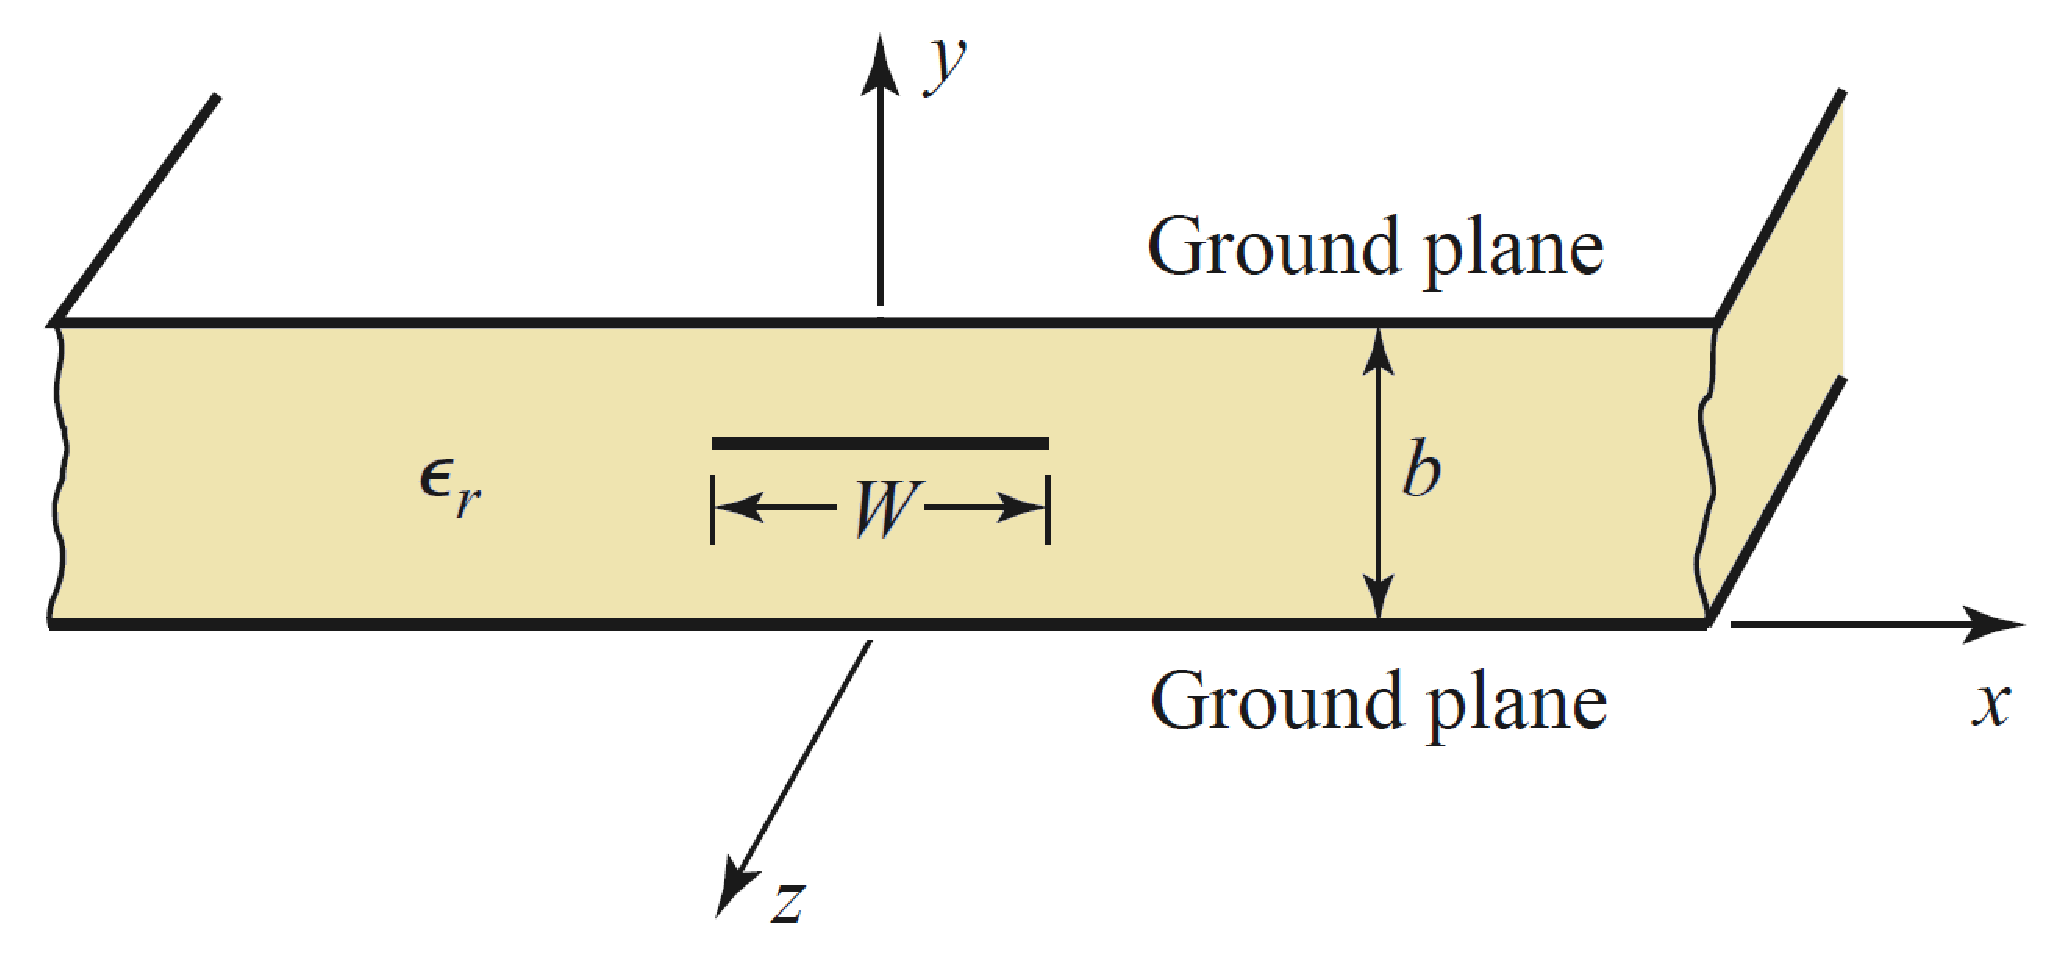
\includegraphics[scale=0.25]{chapter_2/fig3a.eps}\label{th:fig3a} }
\\
\subfloat[] { 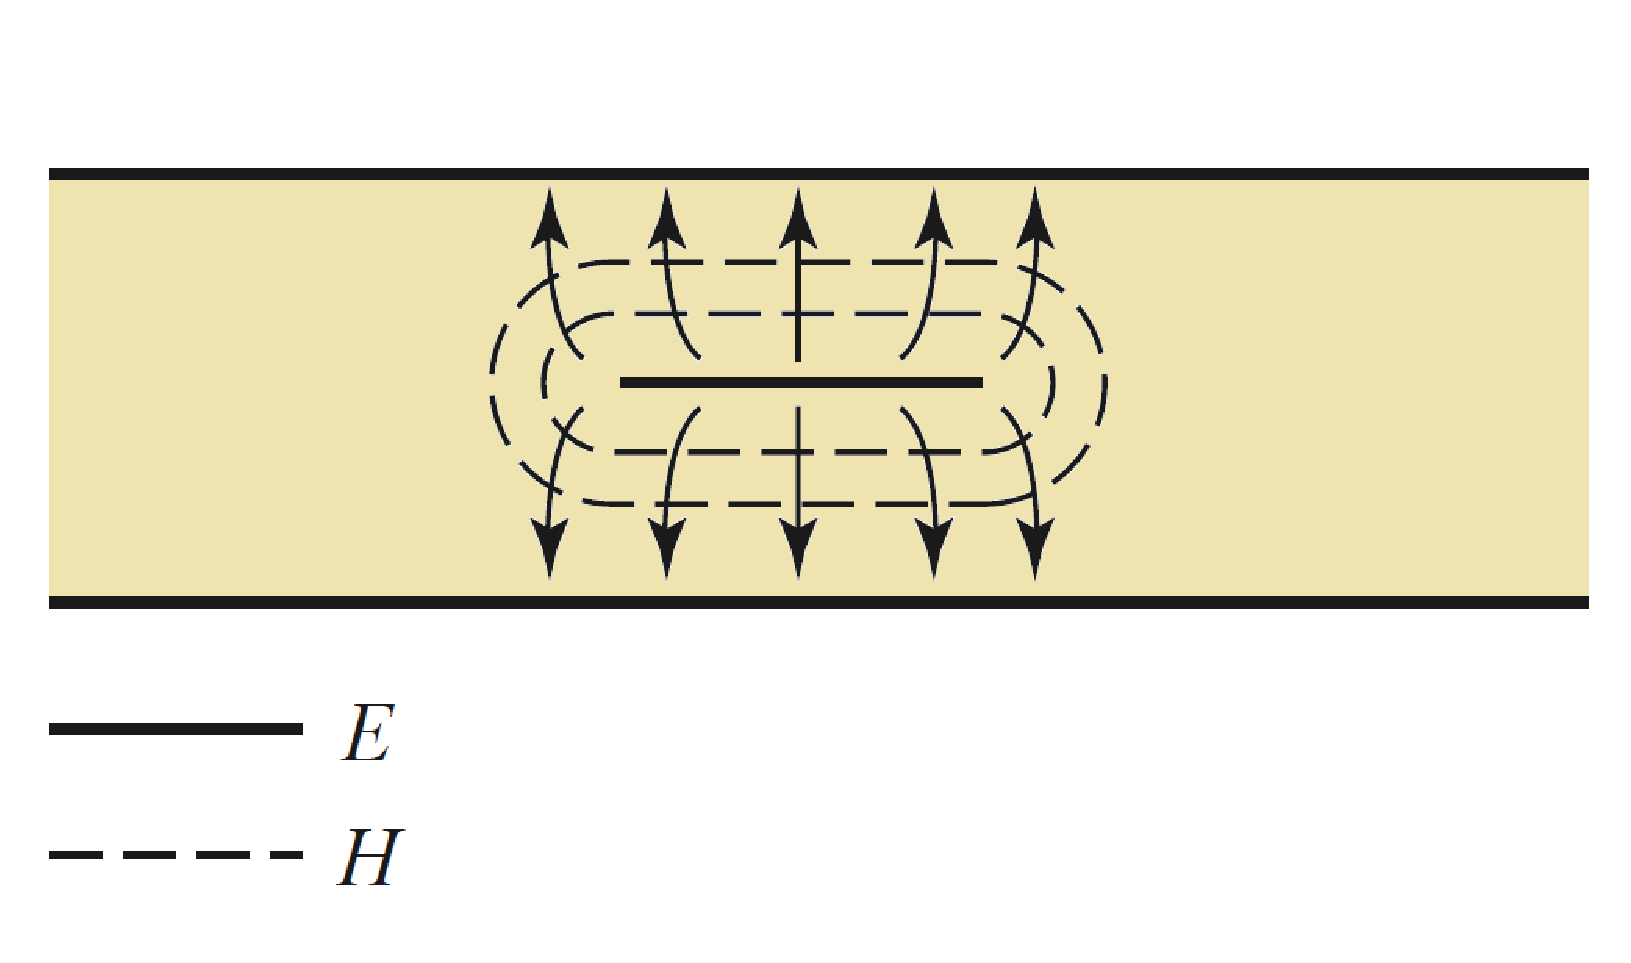
\includegraphics[scale=0.25]{chapter_2/fig3b.eps}\label{th:fig3b} }
\\
\end{tabular}
\caption{Stripline transmission line: geometry (a), electric and magnetic field lines (b).}
\label{th:fig3}
\end{figure}
%%%%%%%%%%%%%%%%%%%%%%%%%%%%%%%%%%%%%%%%%%%%%%%%%%%%%%%%%%%%%

\indent The geometry of stripline is shown in Fig. \ref{th:fig3} together with a sketch of the field lines.  A thin conducting strip of width $W$ is centered between two wide conducting ground planes of separation $b$, and the region between the ground planes is filled with a dielectric material. In practice stripline is usually constructed by etching the center conductor on a grounded dielectric substrate of thickness $b/2$ and then covering with another grounded substrate. Variations of the basic geometry presented in Fig. \ref{th:fig3} include stripline with different dielectric substrate thicknesses (asymmetric stripline) or different dielectric constants (inhomogeneous stripline). Air dielectric is sometimes used when it is necessary to minimize loss.
\\
\indent Since stripline has two conductors and a homogeneous dielectric, it supports a TEM wave, and this is the usual mode of operation. However, stripline can also support higher order waveguide modes. These can usually be avoided in practice by restricting both the ground plane spacing and the sidewall width to less than $\lambda _{d} /2$. Shorting vias between the ground planes are often used to enforce this condition relative to the sidewall width. Shorting vias should also be used to eliminate higher order modes that can be generated when an asymmetry is introduced between the ground planes (e.g., when a surface-mounted coaxial transition is used). A stripline can be considered in a way to be similar to a coaxial transmission line — both have a center conductor completely enclosed by an outer conductor and are uniformly filled with a dielectric medium. 
\\
\indent Because TEM mode of stripline is of primary concern, an electrostatic analysis is sufficient to give the propagation constant and characteristic impedance. Phase velocity can be expressed as:

\begin{equation}\label{th:eq26}
v_{p}=\frac{1}{\sqrt{\mu _{0}\epsilon _{0}\epsilon _{r}}}=\frac{c}{\epsilon _{r}},
\end{equation}

\noindent where $c$ is the speed of light in free-space, and thus the propagation constant of stripline is:

\begin{equation}\label{th:eq27}
\beta =\frac{\omega}{v_{p}}=\omega \sqrt{\mu _{0}\epsilon _{0}\epsilon _{r}}=\sqrt{\epsilon _{r}}k_{0}.
\end{equation}

\noindent The characteristic impedance of a transmission line can be determined under the assumption of very low loss as:

\begin{equation}\label{th:eq28}
Z_{0} =\sqrt{\frac{L}{C}}=\frac{\sqrt{LC}}{C}=\frac{1}{v_{p}C},
\end{equation}

\noindent where $L$ and $C$ are the inductance and capacitance per unit length of the line. Thus, $Z_0$ can be found when knowing $C$.
\\
\indent Since stripline is a TEM line, the attenuation due to dielectric loss can be determined as 

\begin{equation}\label{th:eq29}
\alpha _{d}=\frac{\beta tan\delta }{2} \quad  [Np/m]
\end{equation}

\noindent The attenuation due to conductor loss can be found by the perturbation method or Wheeler’s incremental inductance rule \cite{pozar}. An approximate result is:

\begin{equation}\label{th:eq30}
  \alpha _{c} =
  \begin{cases}
    \frac{2.7x10^{-3}R_{S}\epsilon _{r}Z_{0}}{30\pi (b-t)}A & for\ \sqrt{\epsilon _{r}}Z_{0} < 120\ \Omega \\
    \frac{0.16R_{S}}{Z_{0}b}B  & for\ \sqrt{\epsilon _{r}}Z_{0} > 120\ \Omega
  \end{cases}
 [Np/m]
\end{equation}

\noindent with:

\begin{subequations}\label{th:eq31}
\begin{equation}\label{th:eq31a}
A=1+\frac{W2}{b-t}+\frac{1}{\pi}\frac{b+t}{b-t}ln(\frac{2b-t}{t}),
\end{equation}
\begin{equation}\label{th:eq31b}
B=1+\frac{b}{0.5W+0.7t}(0.5+\frac{0.414t}{W}+\frac{1}{2\pi}ln\frac{4\pi W}{t})
\end{equation}
\end{subequations}

\noindent where $t$ is the thickness of the strip.
\\
% MICROSTRIP

%%%%%%%%%%%%%%%%%%%%%%%%%%%%%%%%%%%%%%%%%%%%%%%%%%%%%%%%%%%%%
\begin{figure}[H]
\centering
\begin{tabular}{c}
\subfloat[] { 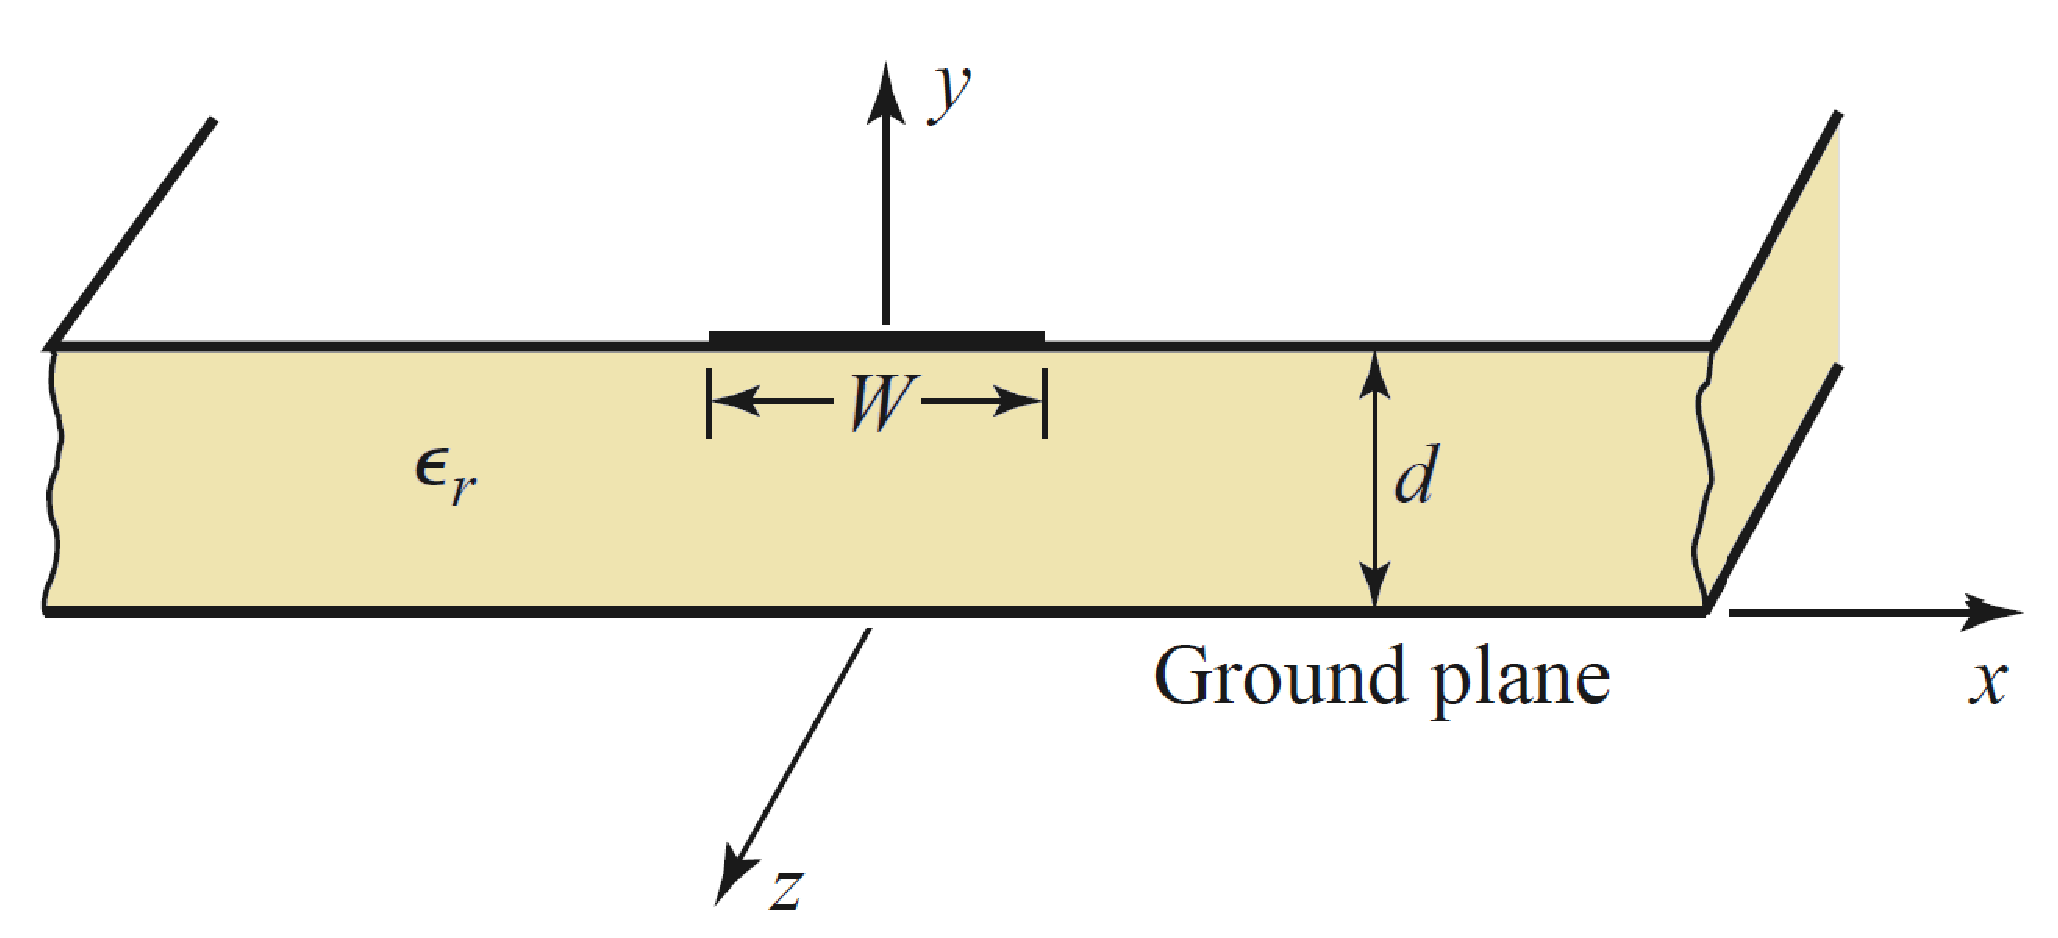
\includegraphics[scale=0.25]{chapter_2/fig4a.eps}\label{th:fig4a} }
\\
\subfloat[] { 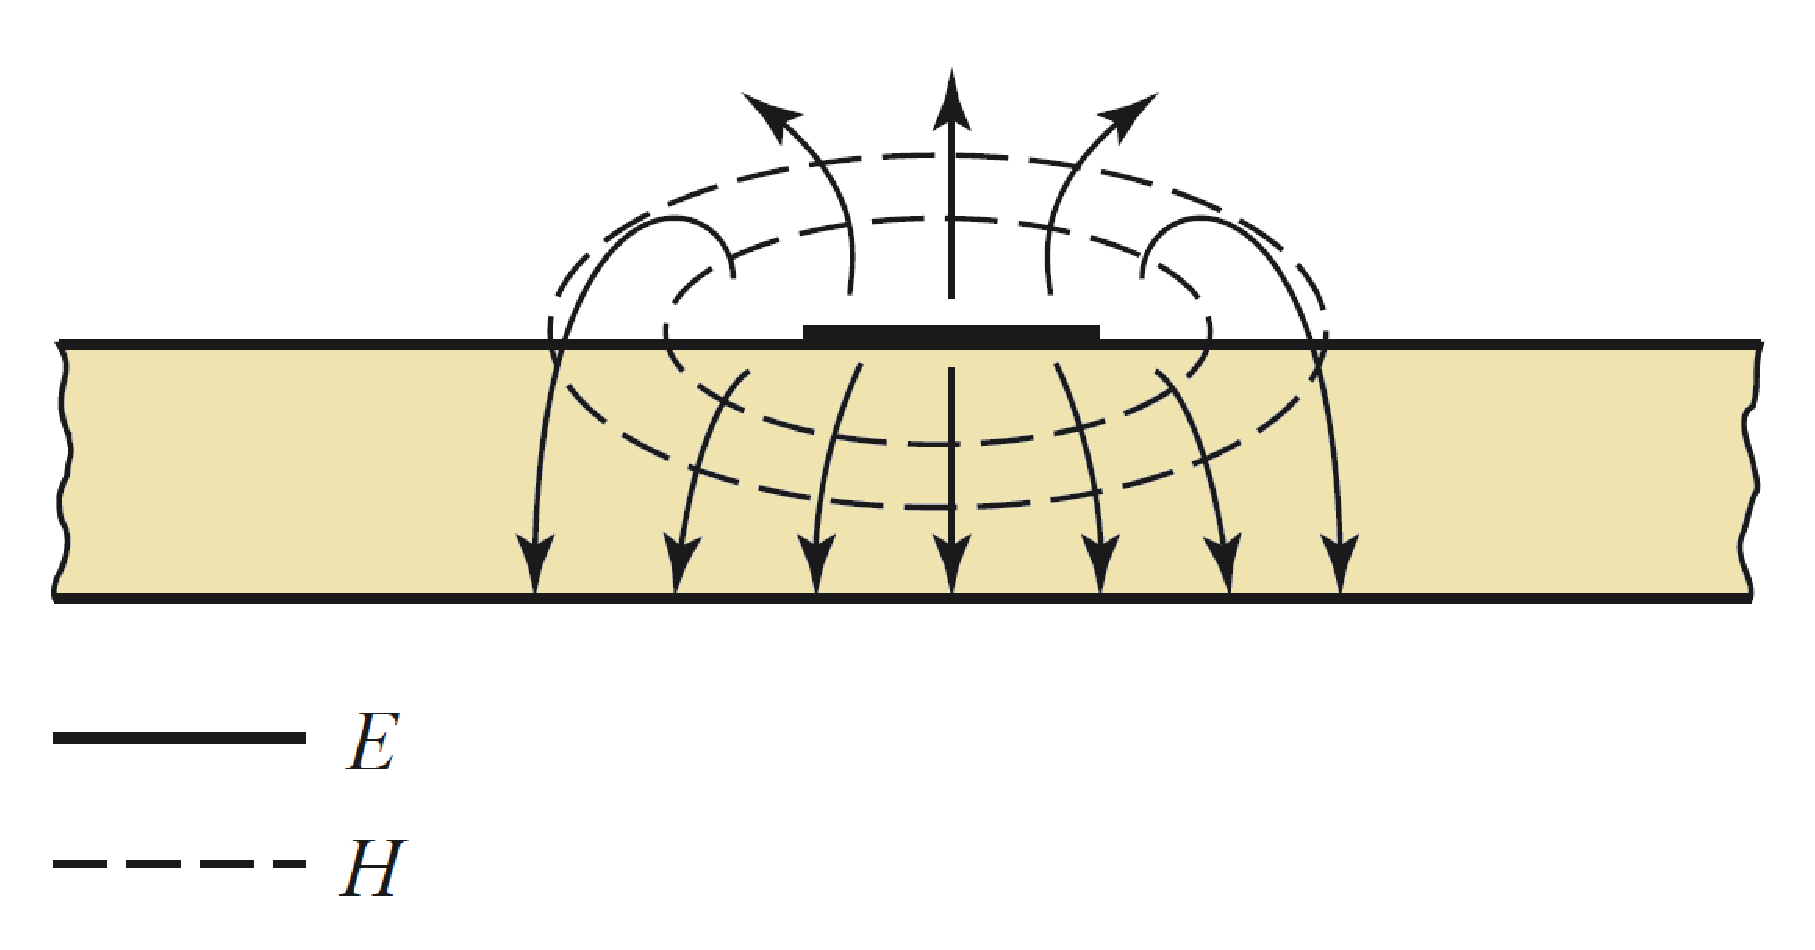
\includegraphics[scale=0.25]{chapter_2/fig4b.eps}\label{th:fig4b} }
\\
\end{tabular}
\caption{Microstrip transmission line: geometry (a), electric and magnetic field lines (b). }
\label{th:fig4}
\end{figure}
%%%%%%%%%%%%%%%%%%%%%%%%%%%%%%%%%%%%%%%%%%%%%%%%%%%%%%%%%%%%%

\indent The geometry of a microstrip line is shown in Fig. \ref{th:fig4} together with a sketch of the field lines. The conductor of width $W$ is printed on a thin, grounded dielectric substrate of thickness $d$ and relative permittivity $\epsilon _{r}$. 
\\
\indent If the dielectric substrate were not present ($\epsilon _{r}$ = 1), microstrip would be a two-wire line consisting of a flat strip conductor over a ground plane, embedded in a homogeneous medium (air). This would constitute a simple TEM transmission line with phase velocity $v_{p} = c$ and propagation constant $\beta = k_0$. 
\\
\indent The presence of the dielectric, particularly the fact that the dielectric does not fill the region above the strip ($y$ > $d$), complicates the behavior and analysis of a microstrip line. Unlike stripline, where all the fields are contained within a homogeneous dielectric region, microstrip has some (usually most) of its field lines in the dielectric region between the strip conductor and the ground plane and some fraction in the air region above the substrate. For this reason microstrip line cannot support a pure TEM wave since the phase velocity of TEM fields in the dielectric region would be $c/\sqrt{\epsilon _{r}}$, while the phase velocity of TEM fields in the air region would be $c$, so a phase-matching condition at the dielectric–air interface would be impossible to enforce.
\\
\indent In actuality, the exact fields of a microstrip line constitute a hybrid TM-TE wave and require more advanced analysis techniques. In most practical applications, however, the dielectric substrate is electrically very thin ($d \ll \lambda $), and so the fields are quasi-TEM. In other words, the fields are essentially the same as those of the static (DC) case. Thus, good approximations for the phase velocity, propagation constant, and characteristic impedance can be obtained from static, or quasi-static, solutions.
Then the phase velocity and propagation constant can be expressed as:

\begin{equation}\label{th:eq32}
v_{p}=\frac{c}{\sqrt{\epsilon _{e}}},
\end{equation}

\begin{equation}\label{th:eq33}
\beta = k_{0}\sqrt{\epsilon _{e}},
\end{equation}

\noindent where $\epsilon _{e}$ is the effective dielectric constant of the microstrip line. Because some of the
field lines are in the dielectric region and some are in the air, the effective dielectric constant satisfies the relation:

\begin{equation}\label{th:eq34}
1 < \epsilon _{e} < \epsilon _{r}
\end{equation}

\noindent and depends on the substrate dielectric constant, the substrate thickness, the conductor
width, and the frequency. The effective dielectric constant of a microstrip line is given approximately by:

\begin{equation}\label{th:eq35}
\epsilon _{e}=\frac{\epsilon _{r}+1}{2}+\frac{\epsilon _{r}-1}{2}\frac{1}{\sqrt{1+12d/W}}.
\end{equation}

\noindent The effective dielectric constant can be interpreted as the dielectric constant of a homogeneous medium that equivalently replaces the air and dielectric regions of the microstrip line. The phase velocity and propagation constant are then given by \ref{th:eq25} and \ref{th:eq26}.
\\
\indent Considering a microstrip line as a quasi-TEM line, the attenuation due to dielectric loss can be determined as:

\begin{equation}\label{th:eq36}
\alpha _{d}=\frac{k_{0}\epsilon _{r}(\epsilon _{e}-1)tan\delta}{2\sqrt{\epsilon _{e}}(\epsilon _{r} -1)} \quad [Np/m],
\end{equation}

\noindent where tan$\delta $ is the loss tangent of the dielectric. The above provided formula account for the fact that the fields around the microstrip line are partially in air (lossless) and partially in the dielectric (lossy). The attenuation due to conductor loss is given approximately by

\begin{equation}\label{th:eq37}
\alpha _{c}=\frac{R_{S}}{Z_{0}W} \quad  [Np/m].
\end{equation}

\noindent For most microstrip substrates, conductor loss is more significant than dielectric loss. Exceptions may occur, however, with some semiconductor substrates.

\cleardoublepage
\chapter{The use of serially connected magnetic tunnel junctions as multistate memory cells.}\label{serspin_mem}
%\chaptermark{test}


\indent In this Chapter

\cleardoublepage

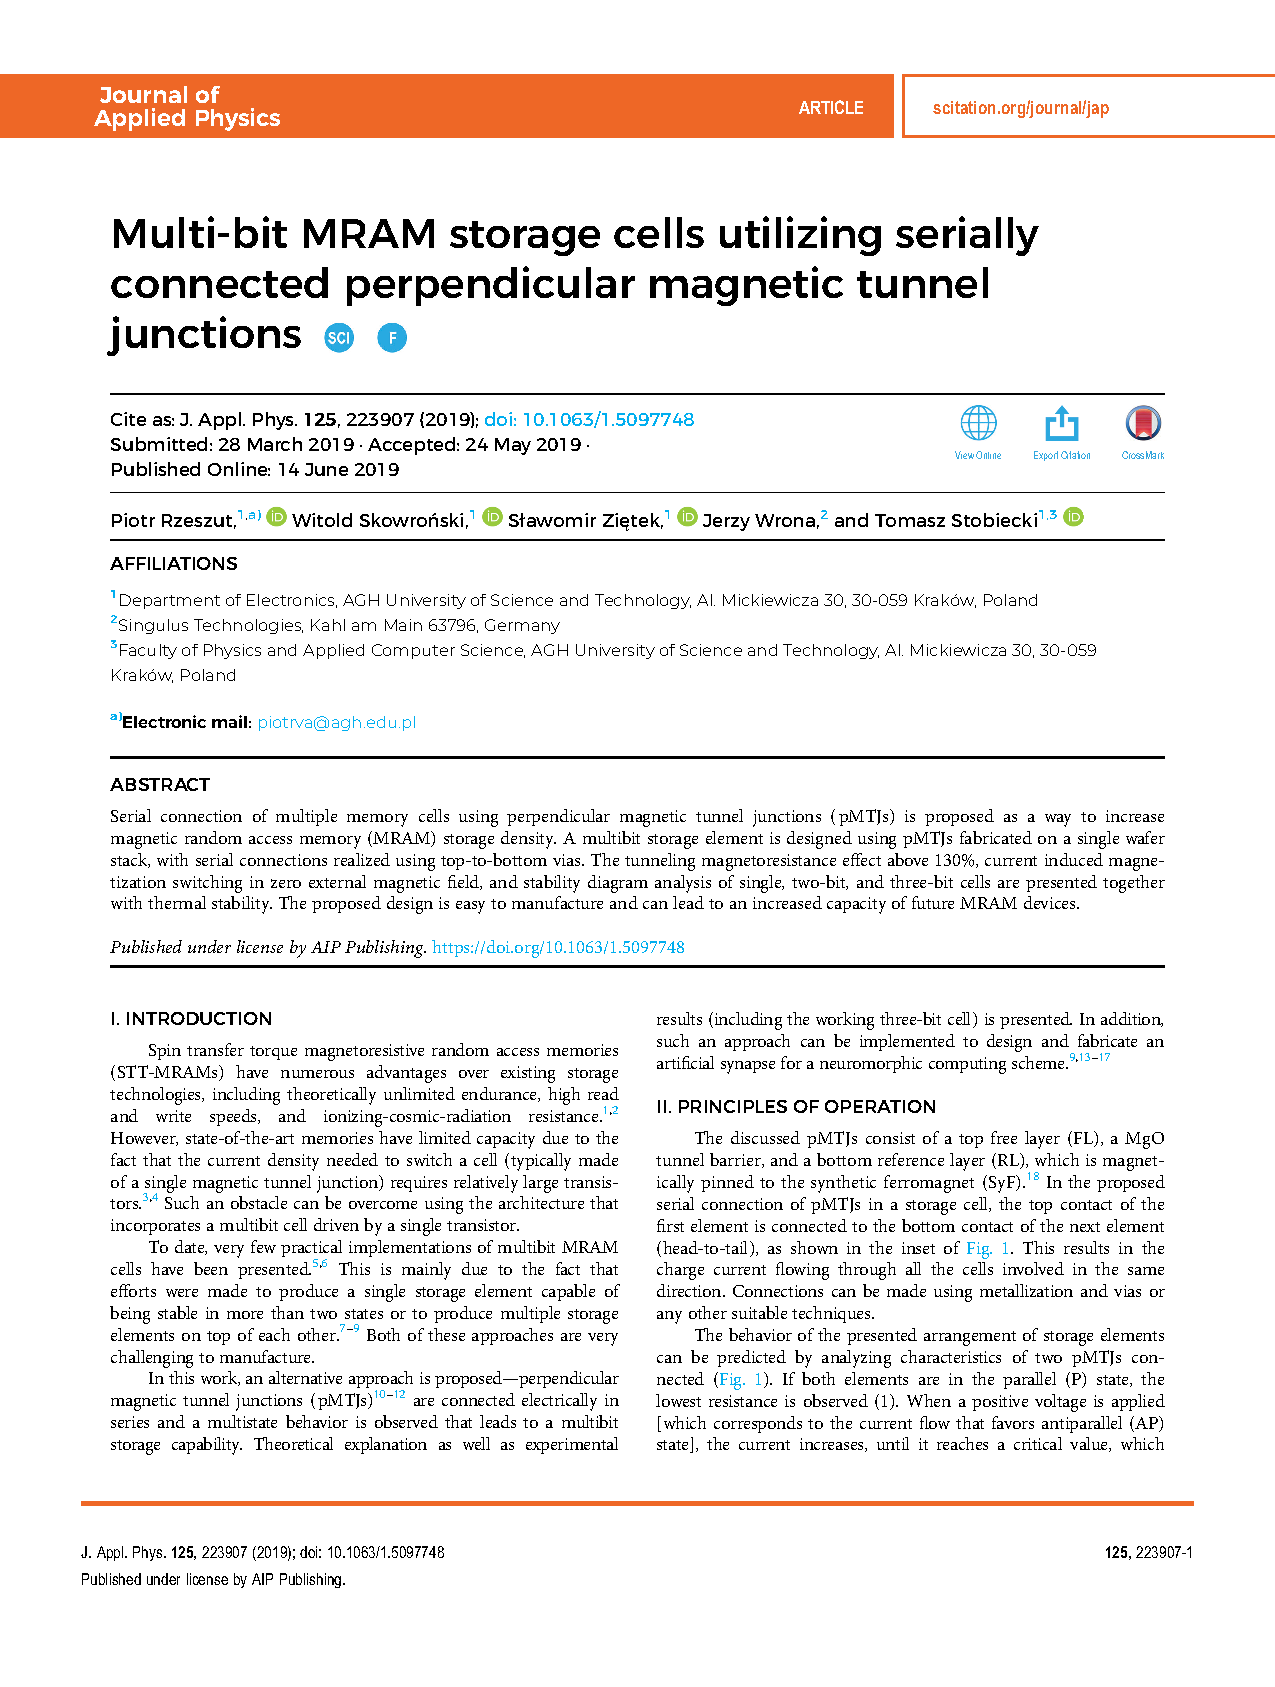
\includepdf[pages=-,addtotoc={1,section,1,Multi-bit MRAM storage cells utilizing serially connected perpendicular magnetic tunnel junctions.,AIP-MRAM}, pagecommand={}, scale=.98]{ch_3/AIP-MRAM_split.pdf}

\cleardoublepage
\chapter{Circuits' topology optimization focused on the performance improvement and functionalities integration as a way of power loss reduction}\label{performance}

\indent In this Chapter the approach of circuits' topology optimization focused on the performance improvement and functionality integration as a way of power loss minimization is presented. More effective circuits' topologies of directional filters and directional couplers were studied allowing to obtain a given required electrical performance while reducing the overall circuits size and/or complexity which as a result leads to the reduction of total length of the wave's propagation path, therefore reduced power loss.
\\
\indent Modern communication systems require an integration of many frequency bands with preferably a single aperture to cover the desired frequencies (e.g., GPS, GSM, WLAN and UWB bands). For such front-end systems, there is a need for broadband antennas on one hand, and devices for multiplexing signals in the frequency domain on the other hand. Devices constructed of directional filters (DFs) can perform multiplexing function \cite{mm_cameron}, while featuring the advantage of low reflection at the input over wide bandwidth and modular topology, in which filters for each band can be designed separately. Furthermore, such devices can easily be integrated with passive and active circuits, effectively increasing system’s integration and lowering the total power loss. Channel selectivity of a multiplexer is dependent from the realization of constitutive DFs, thus highly selective directional filters are of need.
\\
\indent Following the signal path within a wireless transceiver front-end, a power amplification stage is of interest. For low-noise low-power amplifiers MMIC circuits are usually used, whereas for high-power amplifiers, a power transistor based solutions are utilized. Apart from active components, passive power division/summation and/or impedance matching networks are needed, which are rather bulky components. Therefore, a compact and low-loss networks are of importance, hence the integration of power division and impedance transformation functionality \cite{tmtt_wincza_asymmetric_transformers} would be advantageous. Moreover, to allow for realization of broadband amplification stage covering more than one frequency band of interest, broadband directional couplers are required as they are basic components for multi-channel or balanced amplifiers.
\\
\indent The Author has proposed and developed various novel circuits and design methodologies of highly-selective directional filters and frequency multiplexers as well as impedance transforming or broadband directional couplers. Results of the conducted research have been a subject of three journal papers: one submitted to \textit{IEEE Transactions on Microwave Theory and Techniques}, two published in and one submitted to \textit{IEEE Microwave and Wireless Components Letters} and one published in \textit{International Journal of Microwave and Wireless Technologies} as well as two conference papers presented at \textit{International Symposium on Antennas and Propagation ISAP'15} and \textit{International Conference on Microwave, Radar and Wireless Communications MIKON'16}, both under the auspices of \textit{Institute of Electrical and Electronics Engineers IEEE}, which constitute the Chapter.
\\
\indent In Section \ref{pe:isap_df-min}, a new design of a miniaturized coupled-line directional-filters-based multiplexer allowing for band separation in UWB antenna systems has been proposed. To achieve small size of the directional filters, hence the entire multiplexer, directional couplers constituting the filter have been miniaturized following the   approach, in which the coupler is realized as a connection of tightly coupled and uncoupled lines. Moreover, sections of quarter-wave-long transmission lines have been designed with quasi-lumped elements approach, which allows for further miniaturization of the structure. Theoretical analysis of the circuit has been provided. Moreover, performance of the presented approach has been verified by the design and measurement of an exemplary single-channel directional filter multiplexer covering Industrial, Scientific and Medical (ISM) 2.4 GHz band.
\\
\indent Additionally, in Section \ref{pe:mwcl_df-dbrf}, a novel approach to the design of directional filters based on differential bandstop filters and delay lines is proposed. It is shown, that the utilization of a phase inverter and a reference line as a mode converting phase shifter allows for obtaining theoretically ideal bandpass to bandstop channels isolation over an infinite bandwidth. The presented theoretical analysis is confirmed by the realization of an exemplary low-loss directional filter with defected ground type phase inverter covering  ISM 2.4 GHz band. The obtained measurement results show insertion loss as low as 1.1 dB and almost flat isolation response, better than 27 dB up to 6 GHz proving the validity of the presented approach.
\\
\indent Moreover, in Section \ref{pe:tmtt_df-zeros}, a novel topology of a traveling-wave directional filter allowing for selectivity enhancement without increasing filter’s order is proposed. Additional loose cross coupling introduced between $\#(n-1)^{th}$ loop resonator and isolated port of the $n^{th}$-order directional filter allows for generating transmission zeros in the bandpass branch. Moreover, electrical length of the cross coupling connecting transmission line allows for adjusting the location of transmission zeros and realizing symmetric or asymmetric frequency response. The presented approach is theoretically analyzed and experimentally verified. Exemplary second- and third-order directional filters with symmetrically placed transmission zeros were designed to operate at the center frequency $f_0$ = 1 GHz, manufactured and measured. The obtained results prove the correctness and applicability of the presented approach.
\\
\indent Following, in Section \ref{pe:mikon_df-zeros}, a new design of a traveling wave loop directional filter allowing for the realization of transmission zeroes has been proposed. In order to introduce transmission zeroes to bandpass branch of the filter, two loops have been cascaded using transmission line sections. Theoretical analysis of the circuit has been provided giving the insight into behavior of the appearing transmission zeroes related to electrical lengths of the loops’ connecting section. Performance of the presented approach has been verified by the design and measurements of an exemplary cascaded single-loops directional filter with two symmetrically placed transmission zeroes covering ISM 2.4 GHz band. The obtained results proved the usefulness of the presented approach.
\\
\indent Further, in Section \ref{pe:mwcl_multiplexer}, a novel approach to the design of frequency multiplexers consisting of cascaded directional filters is proposed. It is shown that when channels are spaced closely enough, their selectivity can be improved without increasing filters' order by taking advantage of two phenomena. Asymmetric frequency response of a constitutive directional filter allows to increase the attenuation slope on one side of the multiplexer channel. Additionally, the slope on the other side can be increased due to the creation of additional transmission zero resulting from the fact that bandstop response of previous directional filters within the cascade affects directly the response of the following channel. Theoretical analysis is provided together with the applicability condition and multiplexer's design procedure. Moreover, an exemplary four-channel S-band multiplexer was manufactured and measured showing the selectivity improvement of as much as $\sim$ 1.3 times.
\\
\indent Finally, in Section \ref{pe:jmwt_imp-coupler}, a novel impedance transforming directional couplers are proposed in which the achievable impedance transformation ratio is increased above the previously reported limit related to coupling of the coupled-line sections. The proposed couplers consist of two coupled-line sections between which uncoupled sections of LH lines are connected. The presented concept has been verified by circuit simulations as well as by measurements of the manufactured 3-dB coupled-line impedance transforming directional coupler operating at the center frequency $f\textsubscript{0}$ = 1.2 GHz and featuring twofold increase of the impedance transformation ratio compared to a classic solution being $R$ = 4.
\\
\indent Besides, in Section \ref{pe:mwcl_tandem}, a new type of a broadband 3-dB tandem coupler has been proposed featuring frequency characteristics of the resulting coupling similar to these of a classic 3-dB two-section asymmetric coupled-line directional coupler. The coupler is composed of two loosely-coupled-line sections having electrical length close to quarter-wavelength connected by right-handed and left-handed transmission line sections. Theoretical analysis and design equations have been presented with exemplary realization. Measurements of the manufactured tandem coupler operating at the center frequency $f\textsubscript{0}$ = 1 GHz having wide operational bandwidth have been shown to validate the presented analysis.

\cleardoublepage

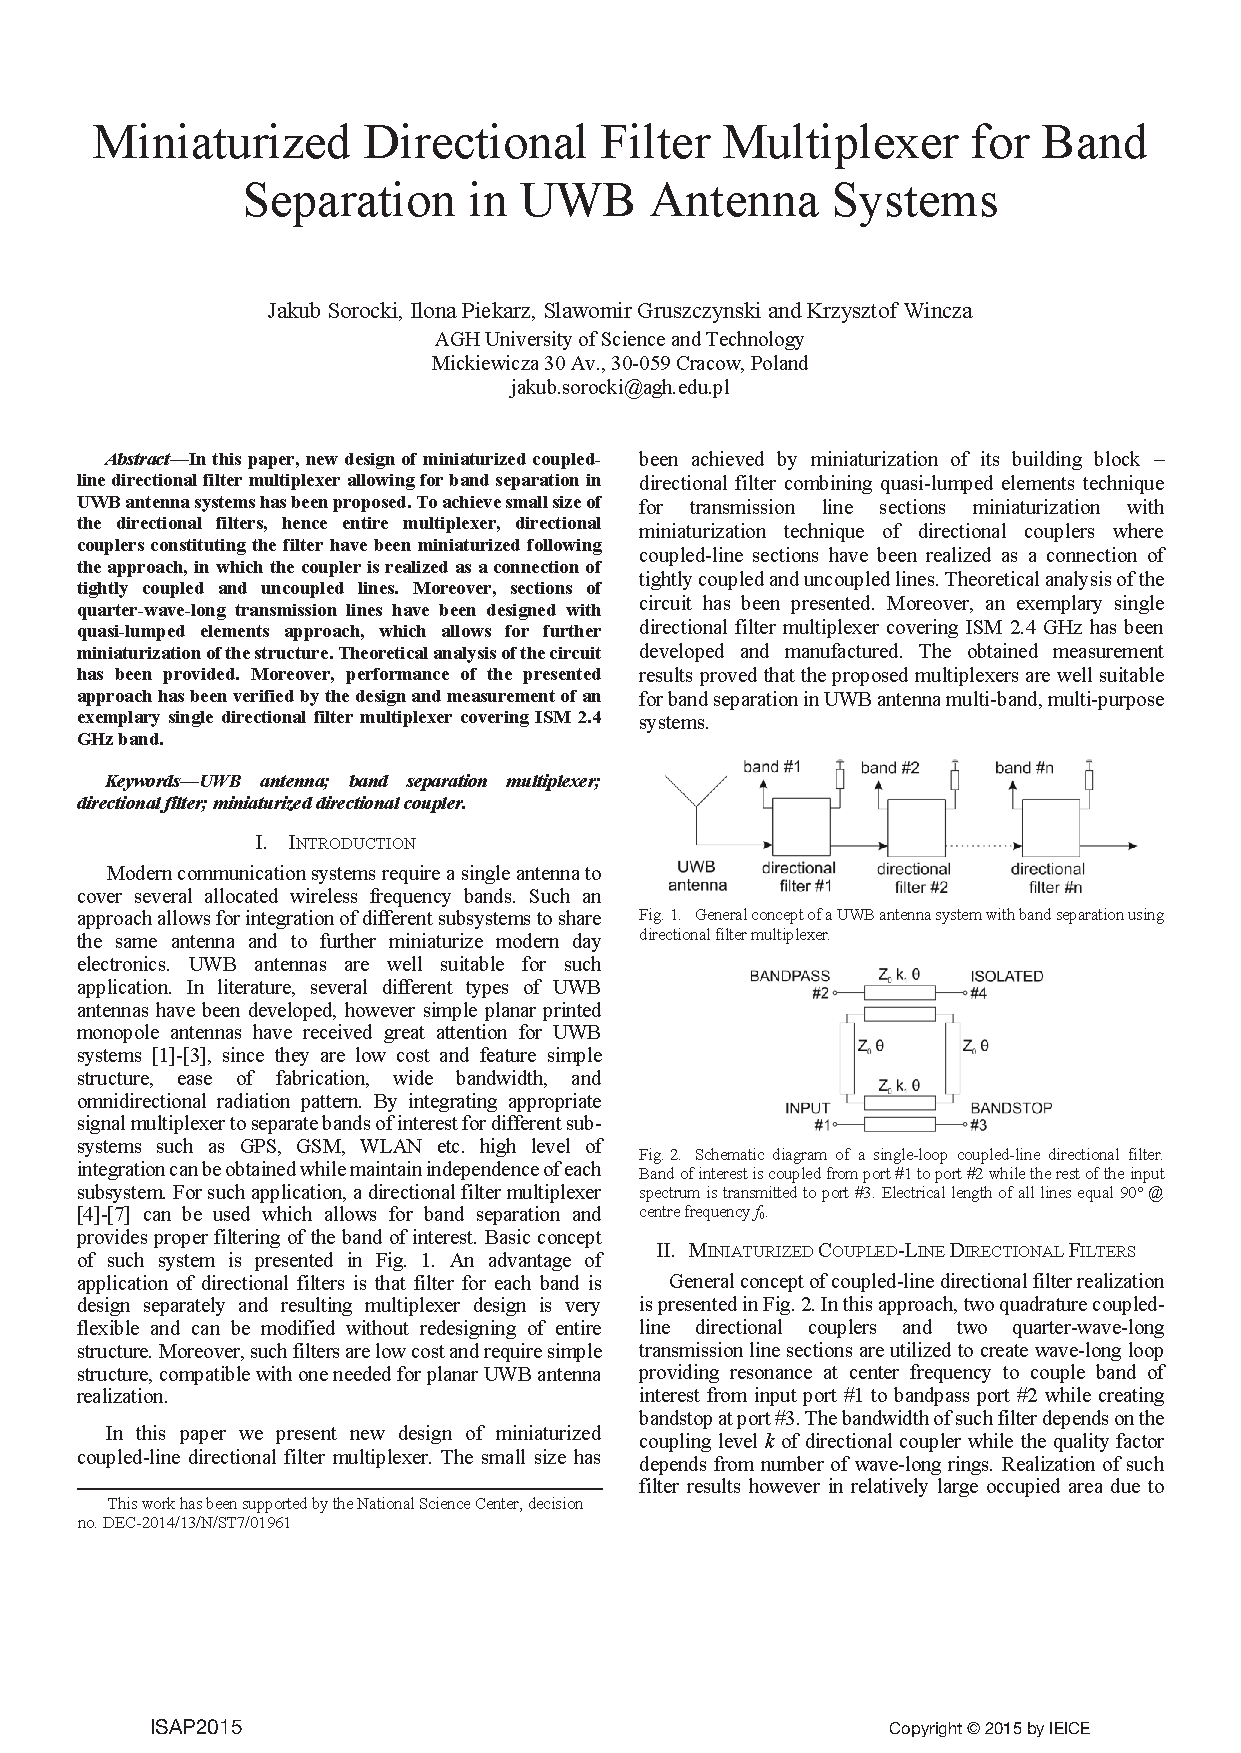
\includepdf[pages=-,addtotoc={1,section,1,Miniaturized directional filter multiplexer for band separation in UWB antenna systems,pe:isap_df-min}, pagecommand={}, scale=.97]{chapter_4/isap_df-min.pdf}

\cleardoublepage

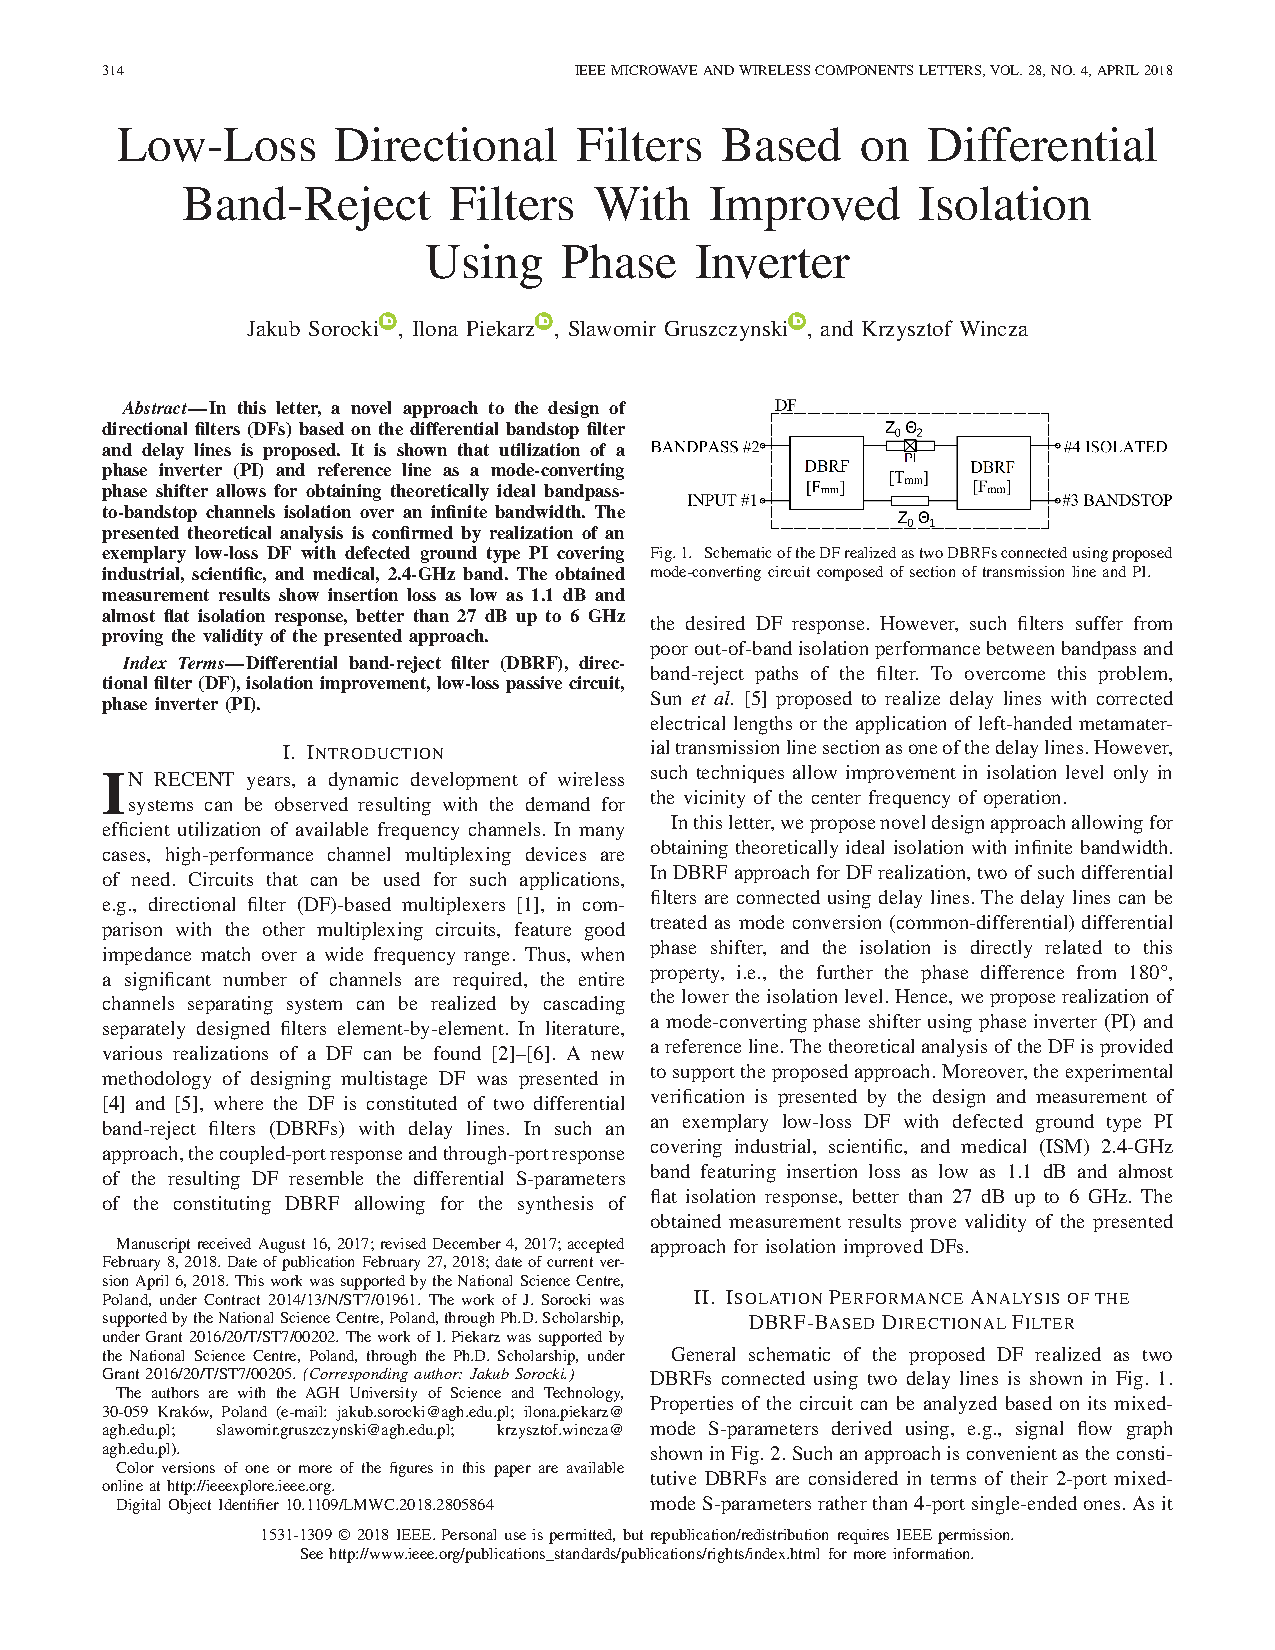
\includepdf[pages=-,addtotoc={1,section,1,Low-loss directional filters based on differential band-reject filters with improved isolation using phase inverter,pe:mwcl_df-dbrf}, pagecommand={}, scale=.97]{chapter_4/mwcl_df-dbrf.pdf}

\cleardoublepage

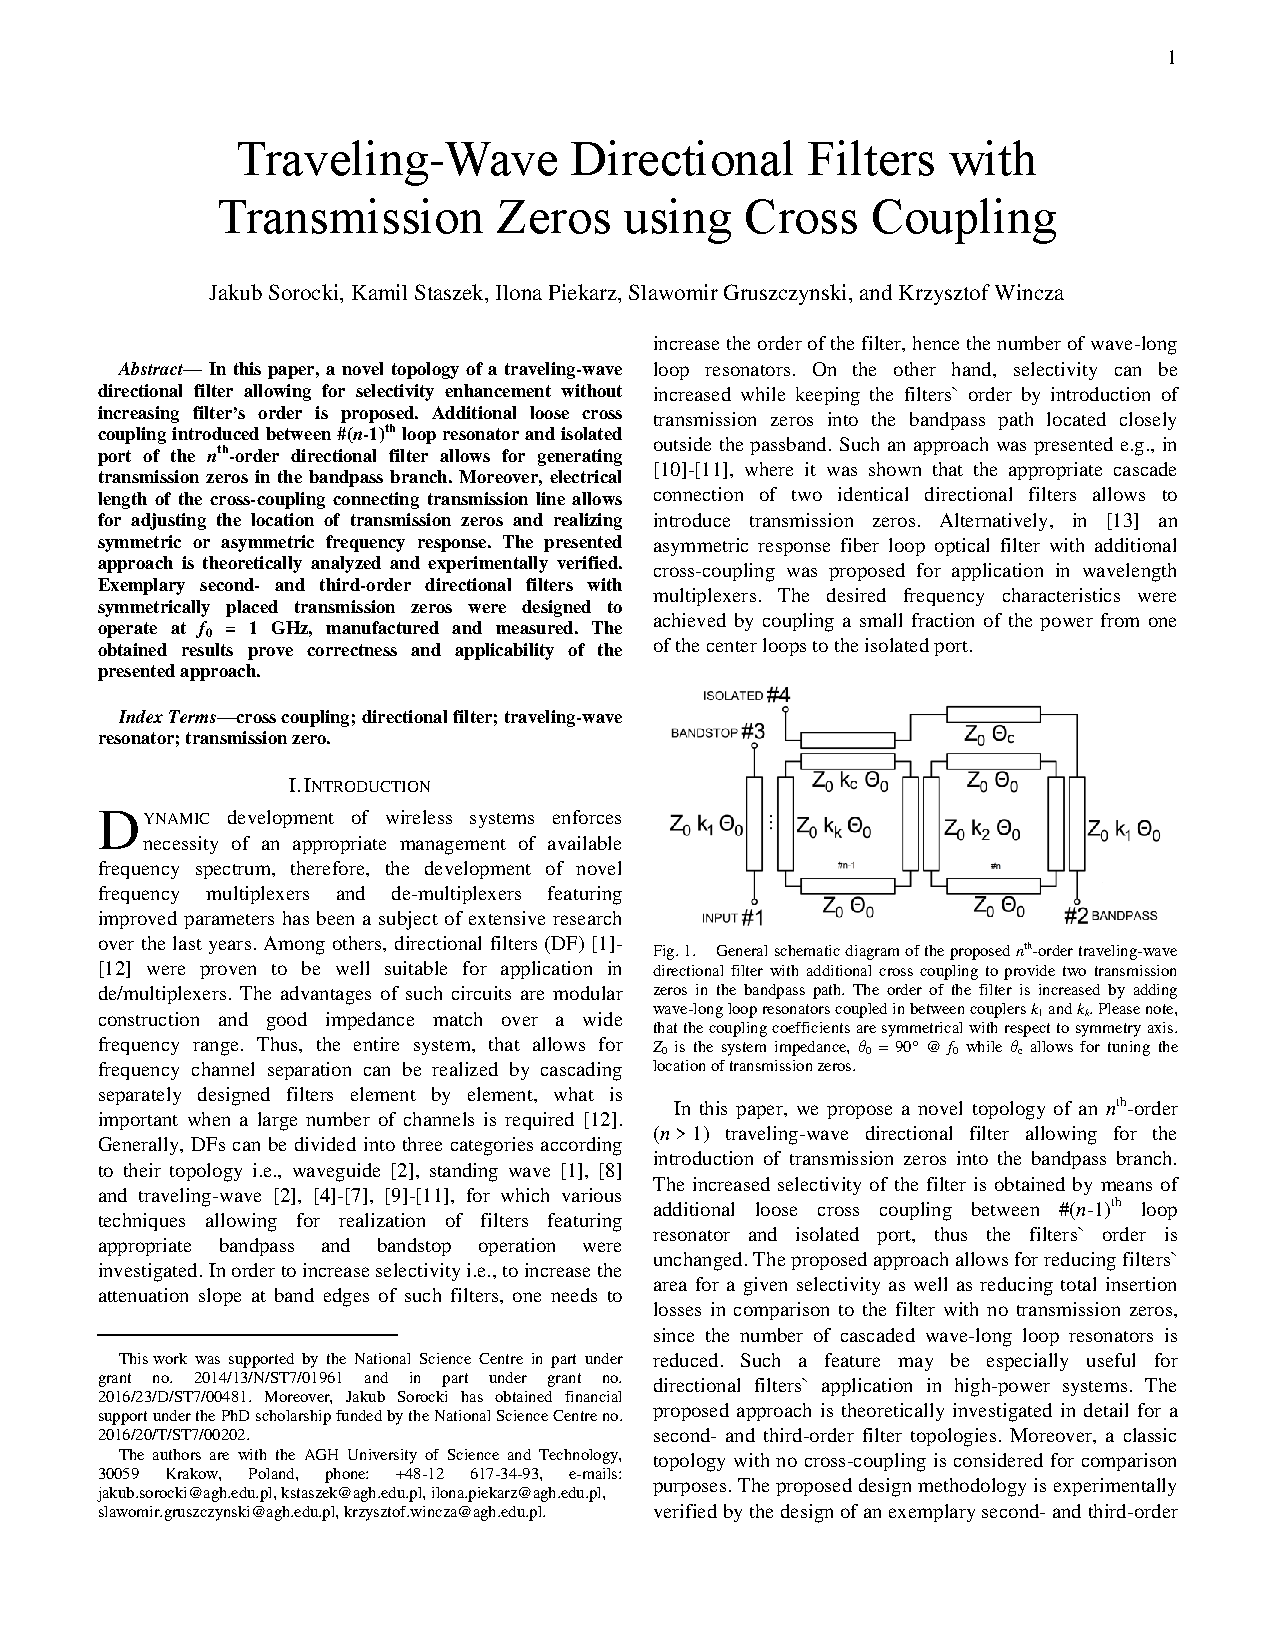
\includepdf[pages=-,addtotoc={1,section,1,Traveling wave directional filters with transmission zeroes using cross coupling,pe:tmtt_df-zeros}, pagecommand={}, scale=.97]{chapter_4/tmtt_df-zeros.pdf}

\cleardoublepage

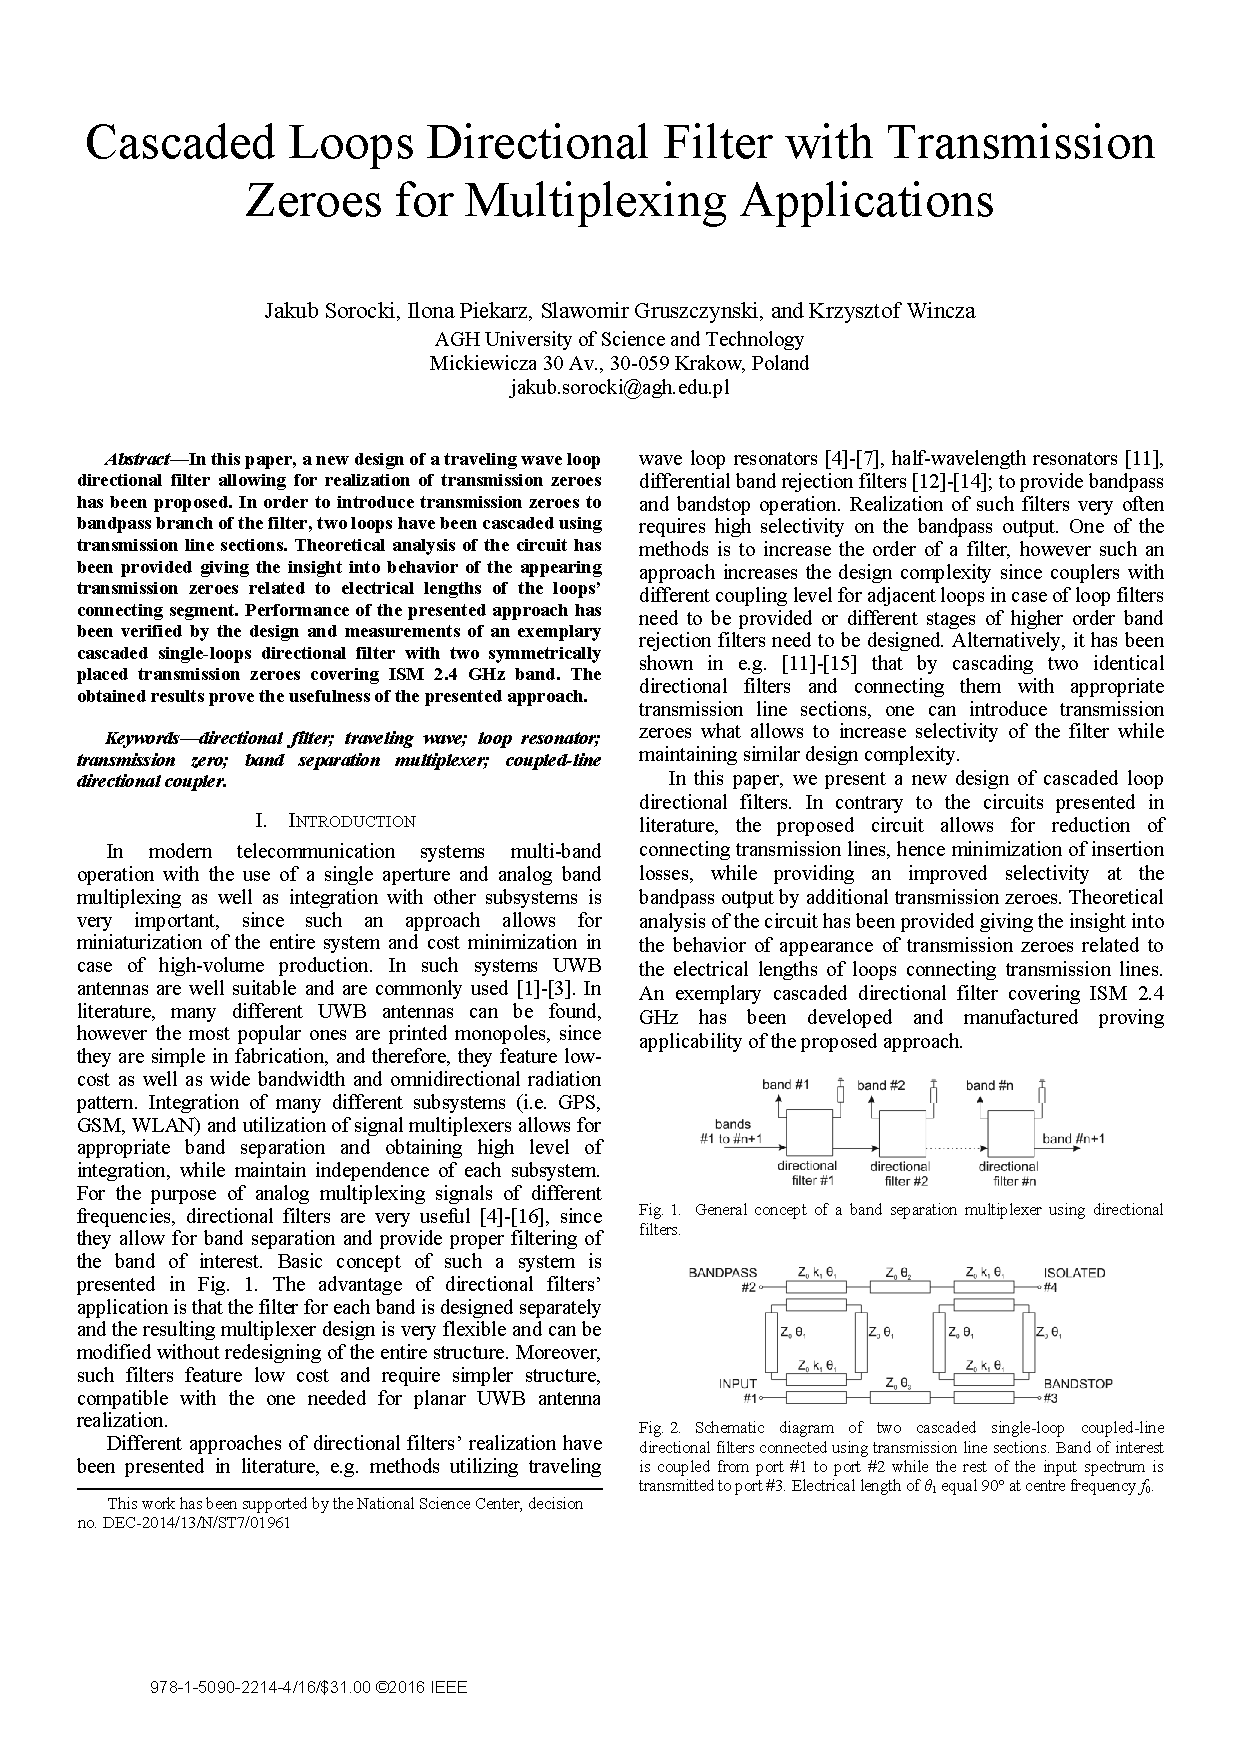
\includepdf[pages=-,addtotoc={1,section,1,Cascaded loops directional filter with transmission zeroes for multiplexing applications,pe:mikon_df-zeros}, pagecommand={}, scale=.97]{chapter_4/mikon_df-zeros.pdf}


\cleardoublepage

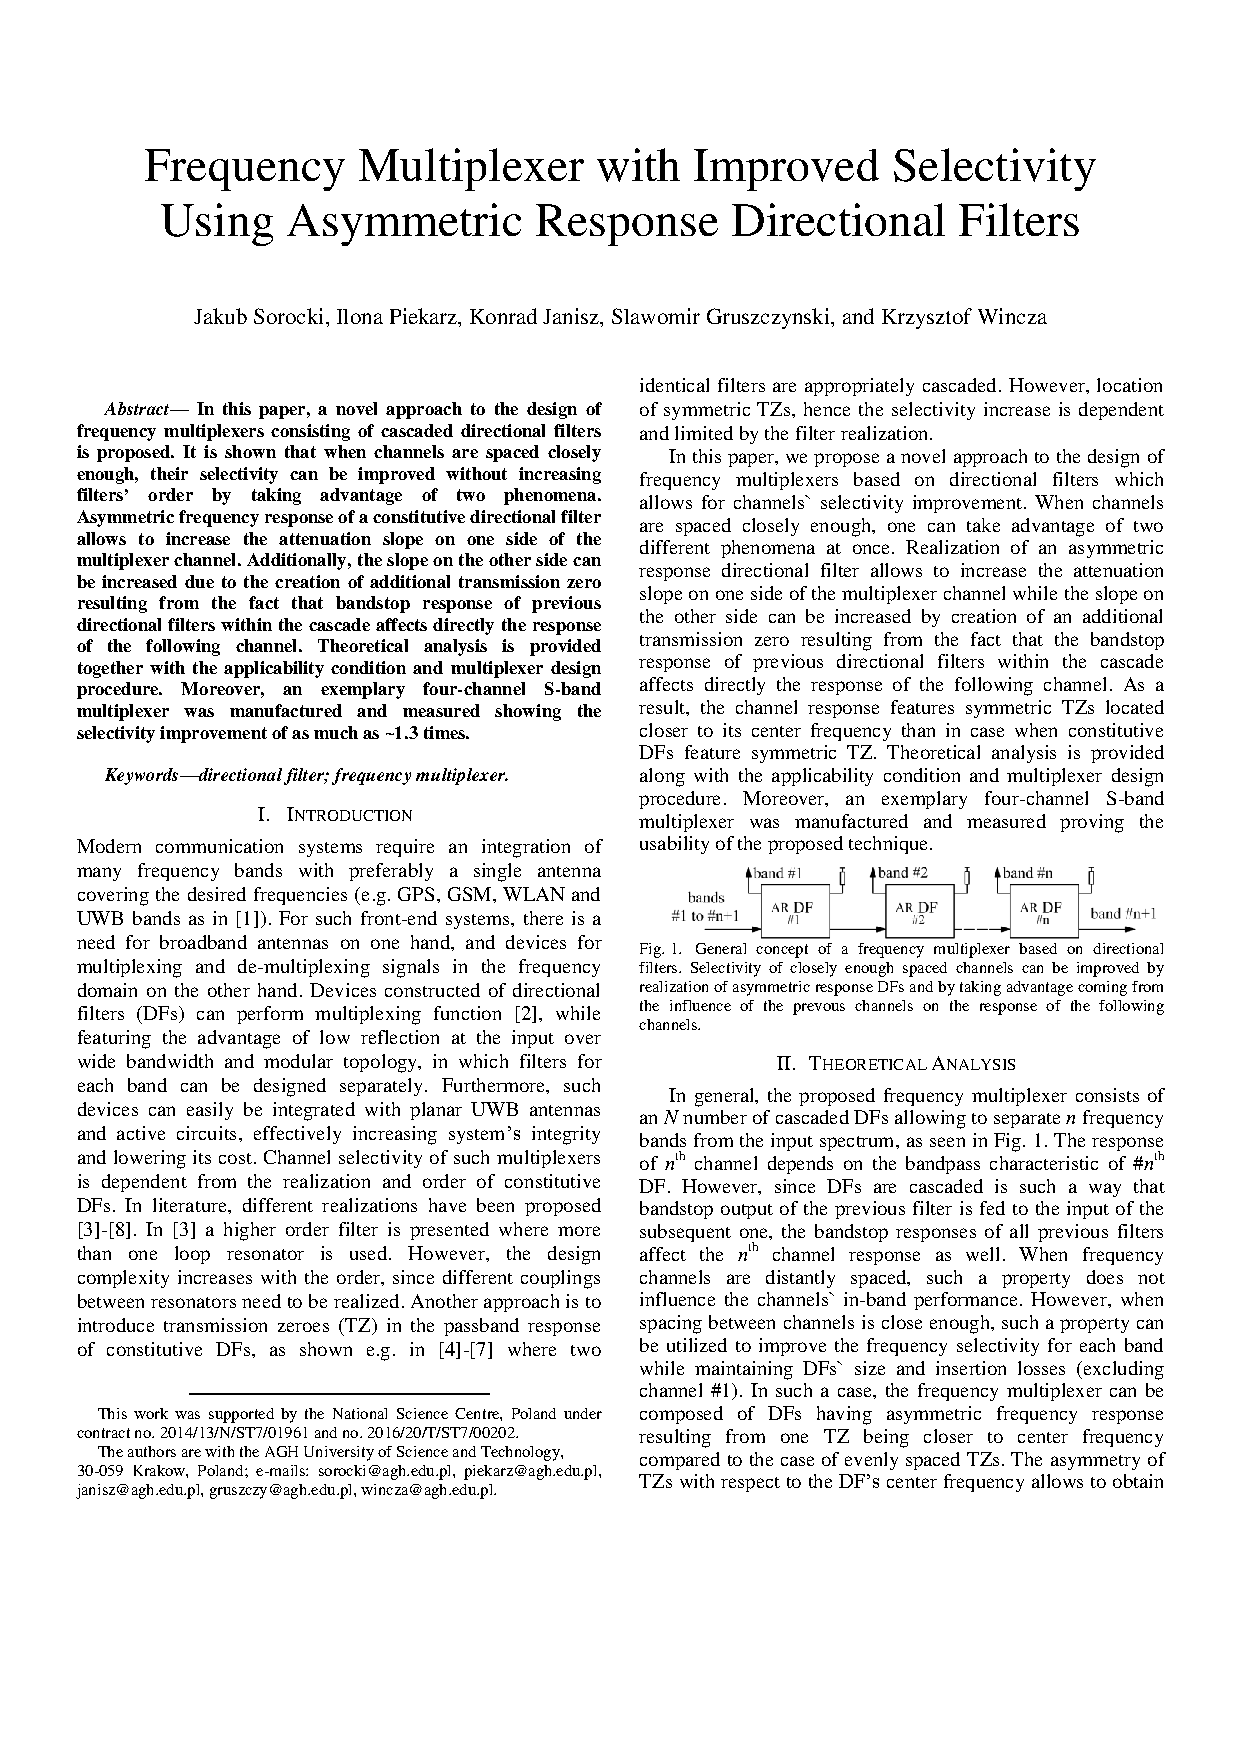
\includepdf[pages=-,addtotoc={1,section,1,Frequency multiplexers with improved selectivity using asymmetric response directional filters,pe:mwcl_multiplexer}, pagecommand={}, scale=.97]{chapter_4/mwcl_multiplexer.pdf}

\cleardoublepage

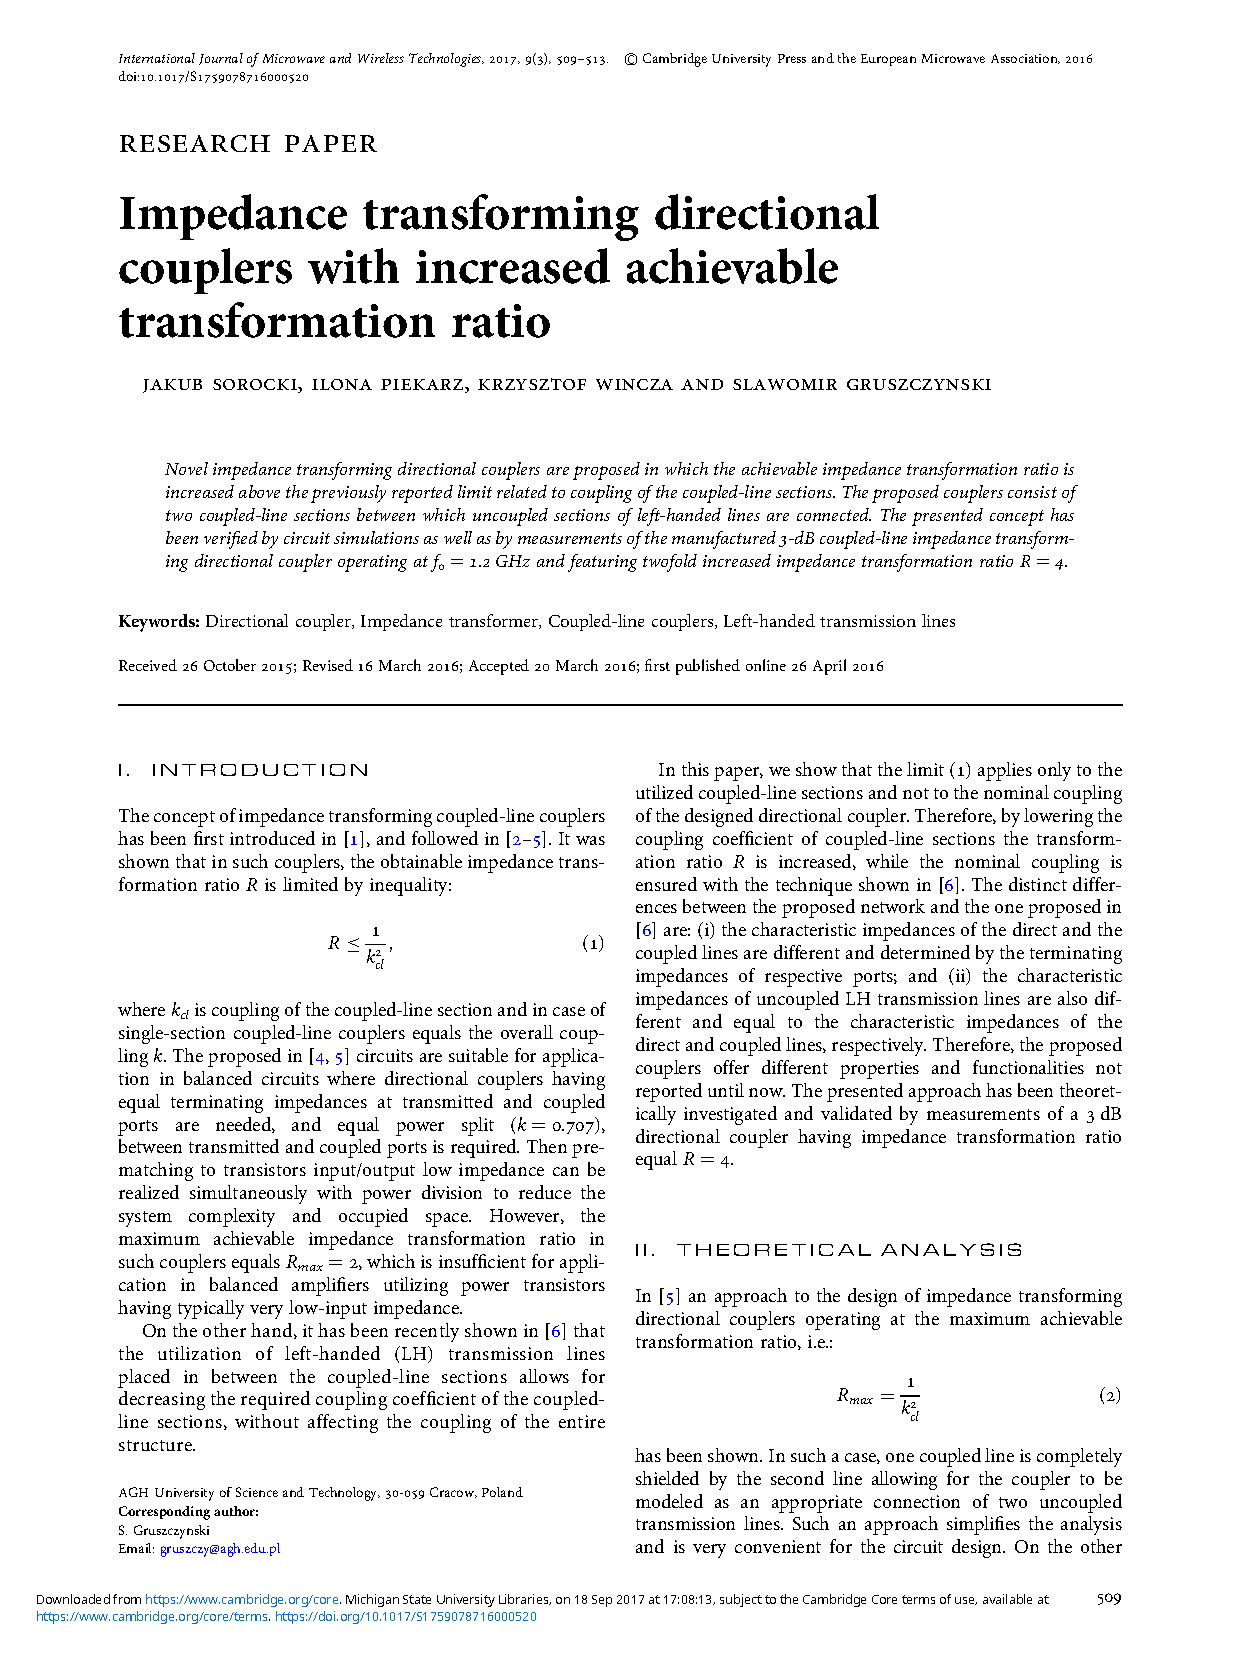
\includepdf[pages=-,addtotoc={1,section,1,Impedance transforming directional couplers  with increased achievable transformation ratio,pe:jmwt_imp-coupler}, pagecommand={}, scale=.97]{chapter_4/jmwt_imp-coupler.pdf}

\cleardoublepage

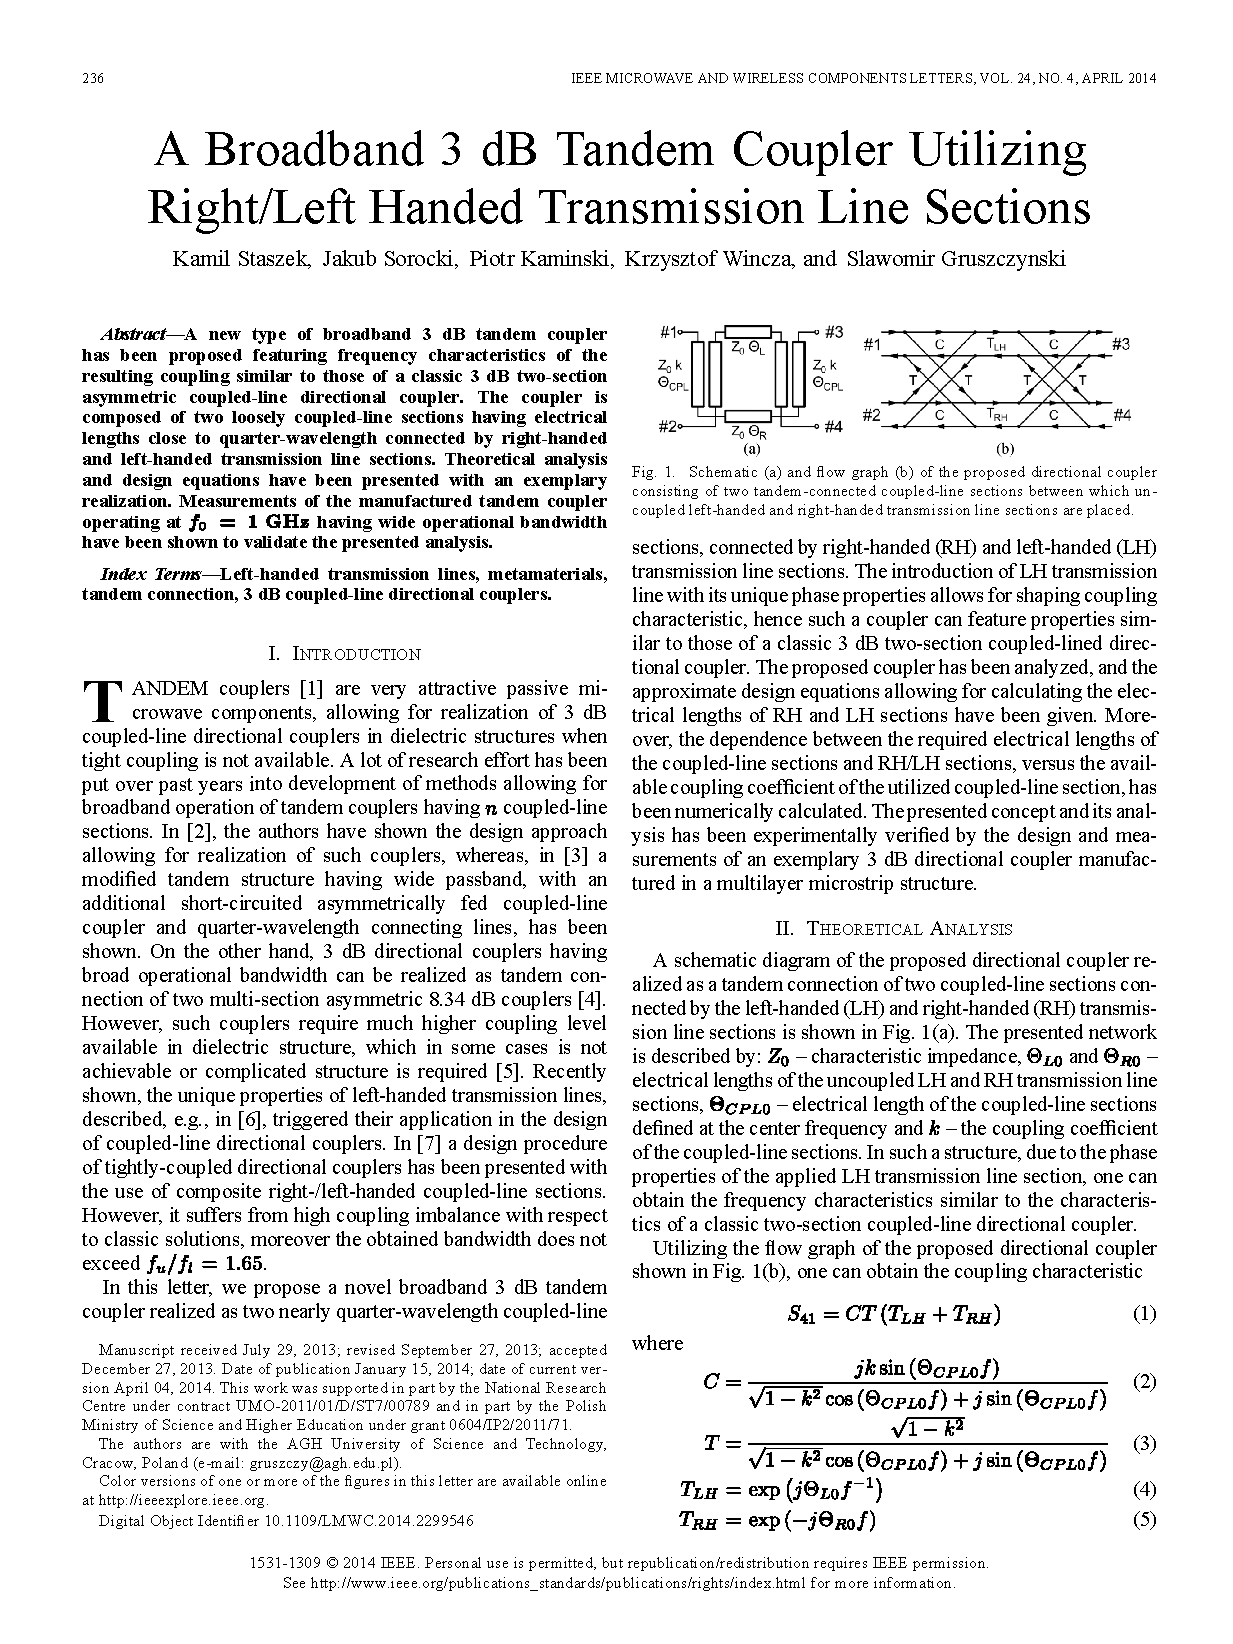
\includepdf[pages=-,addtotoc={1,section,1,A broadband 3 dB tandem coupler utilizing right/left handed transmission line sections,pe:mwcl_tandem}, pagecommand={}, scale=.97]{chapter_4/mwcl_tandem.pdf}

\cleardoublepage

%\includepdf[pages=-,addtotoc={1,section,1,Broadband balun circuits composed of impedance transforming directional couplers and LH transmission-line sections,tmtt_right_left}]{chapter_4/jiee.pdf}

%\cleardoublepage
\chapter{Introduction of emerging manufacturing technologies and novel materials for low-loss circuits' realization}\label{emerging}

\indent In this Chapter the application of emerging materials and manufacturing technologies for the realization of low loss microwave circuits in strip transmission line technique is considered and discussed. Application of various 3D printing technologies and dedicated materials are the subject of this study, including Fused Deposition Modeling (FDM) and Poly Jet Printing (PJP) as well as wide variety of conductive and dielectric materials.
\\
\indent Initially adopted for rapid prototyping to test the design before the final product development, additive manufacturing (AM) technologies have rapidly evolved toward the complete (one-pass) manufacturing of end-use components \cite{pieee_sorrentino}. This is due to significant development of the manufacturing equipment as well as material engineering. Recently also RF engineers have started to leverage AM technologies, including 3D printing, to develop the next generation of microwave and millimeter-wave devices aimed at several applications operating from hundreds of megahertz to hundreds of gigahertz, among which are millimeter-wave wireless and satellite communication systems and components such as waveguides, sensors, antennas, filters, power dividers, etc.. In such areas, AM offers several advantages such as design and geometrical flexibility of the circuits superior to conventional 2.5D techniques due to three-dimensional nature of the technology, near-net shape manufacturing, reduced tooling and fixtures, and almost no process waste. Moreover, another enabling advantage of AM processes is that it allows for the realization of multifunction parts, which means that several functionalities (electrical, thermal, or structural) are implemented in a single object. Finally, compared to conventional machining techniques, AM can be applied to produce custom microwave devices at reduced lead time and costs. 
\\
\indent The Author has experimentally investigated various additive manufacturing technologies and dedicated materials in terms of low-loss stripline microwave circuits realization as well as developed novel circuits taking advantage of the recent developments in technology and material engineering. The results of the conducted research have been a subject of one journal paper submitted to \textit{IEEE Transactions on Microwave Theory and Techniques} and three conference papers presented at \textit{International Conference on Electrical, Electronics and System Engineering (ICEESE'17)} and \textit{Electronic Components and Technology Conference (ECTC'18)}, all under the auspices of \textit{Institute of Electrical and Electronics Engineers}, which constitute the Chapter.
\\
\indent In Section \ref{iceese_graphene}, the applicability of additive manufacturing with conductive Polylactic Acid (PLA) based filament for the realization of low-loss suspended microstrip microwave circuits is investigated. Filament is used to 3D print a case which serve three major functions: provides mechanical enclosure and support for the circuit, provides appropriate elevation of the thin laminate with a circuit's pattern over the ground plane and can potentially serve as a ground plane. The influence of the bulk conductivity of the utilized filament on total losses within the structure has been studied. Moreover, an exemplary transmission line hosted in Fused Deposition Modelling (FDM) 3D printed case has been manufactured and measured. Graphene-enhanced PLA material having volume conductivity of $\sim$ 166 S/m has been used yielding total loss of $\sim$ 0.14 dB/cm/GHz while reference case with copper foil ground plane yields total loss of $\sim$ 0.04 dB/cm/GHz.
\\
\indent Following, in Section \ref{ectc_electr}, the realization of microwave circuits in suspended microstrip structure with a 3D printed conductive enclosure is presented. An example of a low-pass filter with a cut-off frequency of 2.5 GHz was designed, manufactured and measured. A Fused Deposition Modeling (FDM) type 3D printing and a conductive copper-based filament recently developed by Multi 3D featuring superior conductivity over BlackMagic 3D's Graphene-enhance PLA were employed to realize an enclosure serving both mechanical and electrical purposes. The influence of the ground plane conductivity on the total loss within the circuit was studied, and requirements for the conductive material properties were established. Moreover, the impact of the print parameters as well as the connection between microstrip line and SMA connectors were investigated. The obtained measurements proved that the proposed approach is of potential use for circuits and systems operating within low GHz frequency range.
\\
\indent Moreover, in Section \ref{ectc_df-poly}, an application of additive manufacturing technologies for realization of multilayer microwave circuits in microstrip transmission line technique is presented. An example of a second-order cascaded loops directional filter allowing to separate 2100 MHz Long-Term Evolution (LTE) band was designed in suspended microstrip technique with three metal layers, manufactured using a combination of PolyJet 3D printing with UV cured VeroWhitePlus polymer material and magnetron sputtering of copper, and assembled out of two parts using a “lego-like” process. The obtained results for the manufactured circuit were evaluated in terms of electrical performance and total power loss showing that the proposed approach is of potential use for circuits and systems operating within the microwave frequency range.
\\
\indent Finally, in Section \ref{tmtt_right_left}, a novel approach for the realization of high-performance coupled-line directional couplers in suspended stripline technique is proposed taking advantage of recent development in 3D printing technology. A third degree of freedom is introduced to a 2.5D structure allowing to combine the advantages of strip-transmission-line techniques, for which the circuit can still be considered as a quasi-planar structure, with the 3D printing flexibility of air layer thickness variation limited only by technological constraints. It is shown, that the proposed approach is well suitable for the realization of low-loss circuits, where tight coupling and superior performance and compactness are required. Moreover, it is shown that compensating elements, often required to improve couplers' performance, can easily be realized as a combination of a circuit's pattern and ground plane integrated 3D structures allowing for better circuit's volume utilization. An example of a 3-dB coupled-line directional coupler operating within the ISM 5.8 GHz band is designed, manufactured and measured for experimental verification. The obtained results have shown high electrical performance and low power losses of the circuit confirming the applicability of the proposed approach.

\cleardoublepage

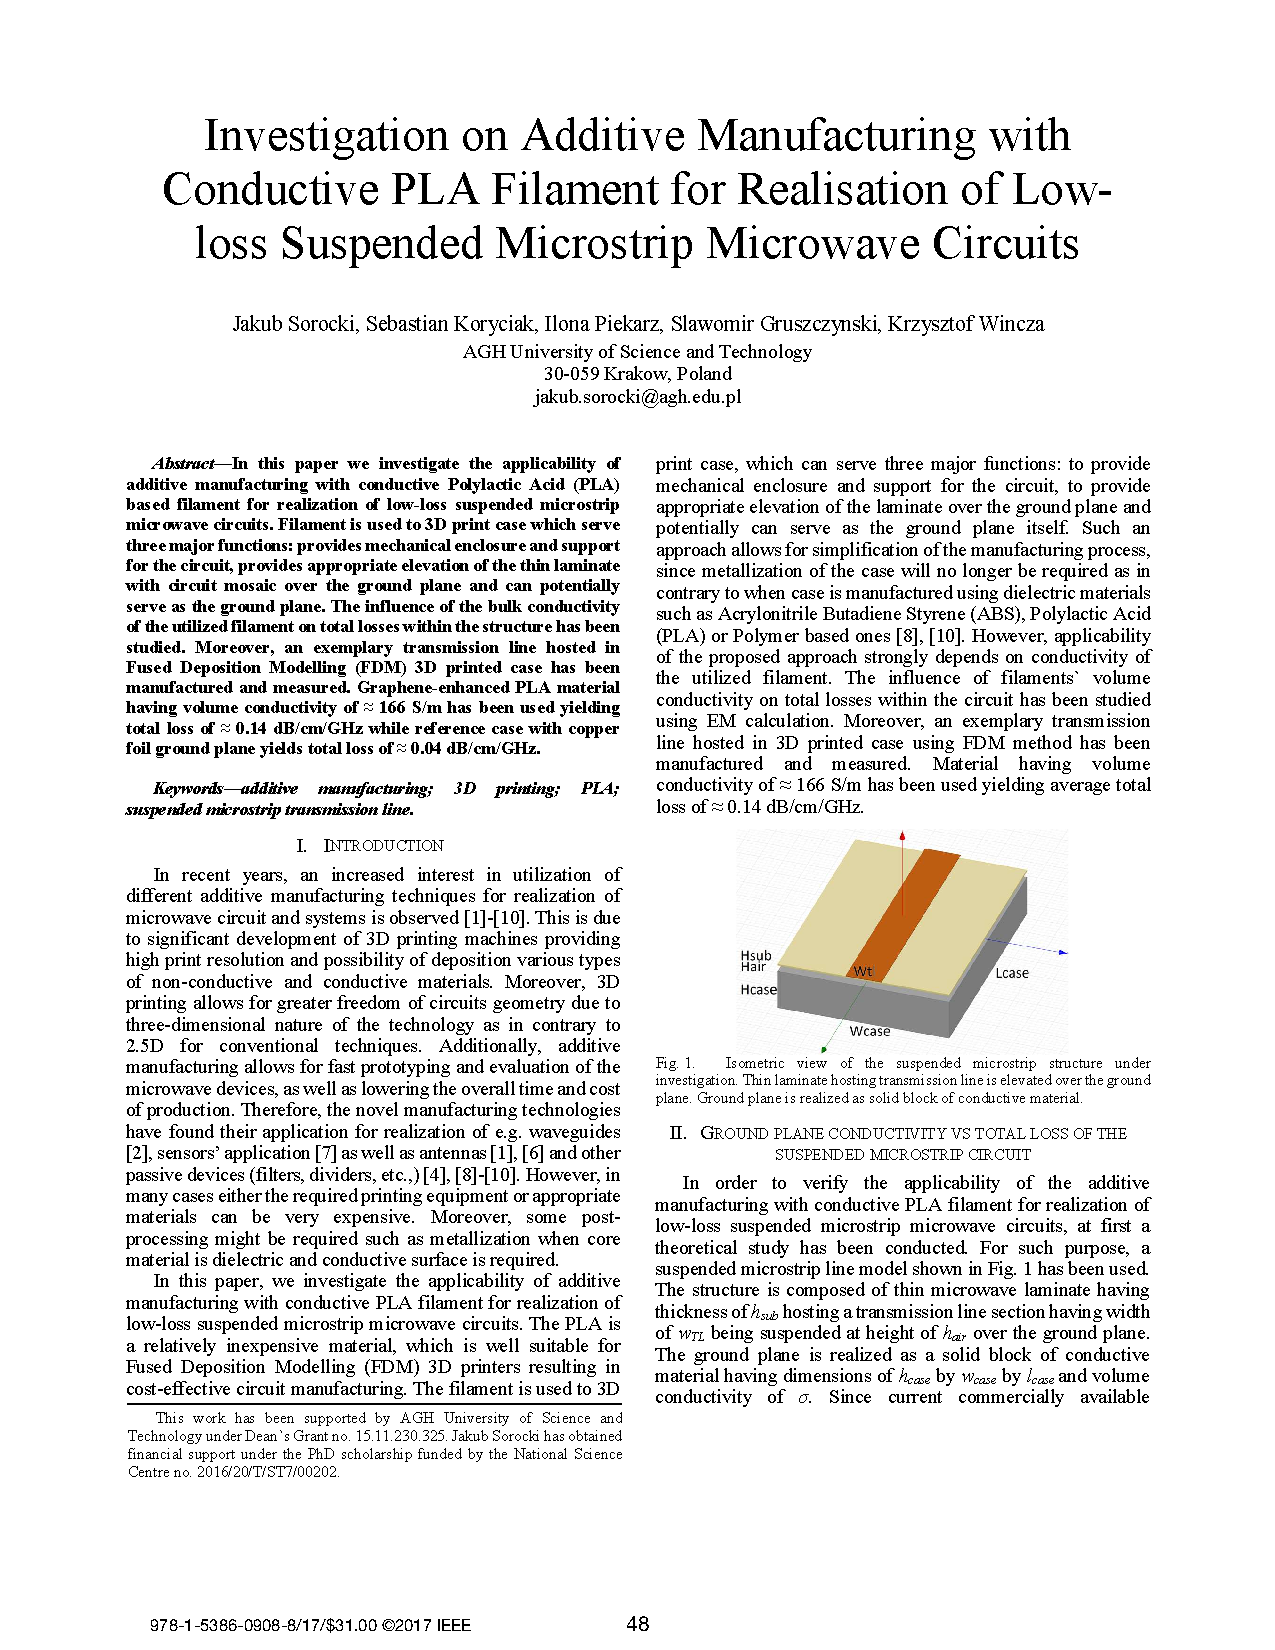
\includepdf[pages=-,addtotoc={1,section,1,Investigation on additive manufacturing with conductive PLA filament for realisation of low-loss suspended microstrip microwave circuits,iceese_graphene}, pagecommand={}, scale=.97]{chapter_5/iceese_graphene.pdf}

\cleardoublepage
 
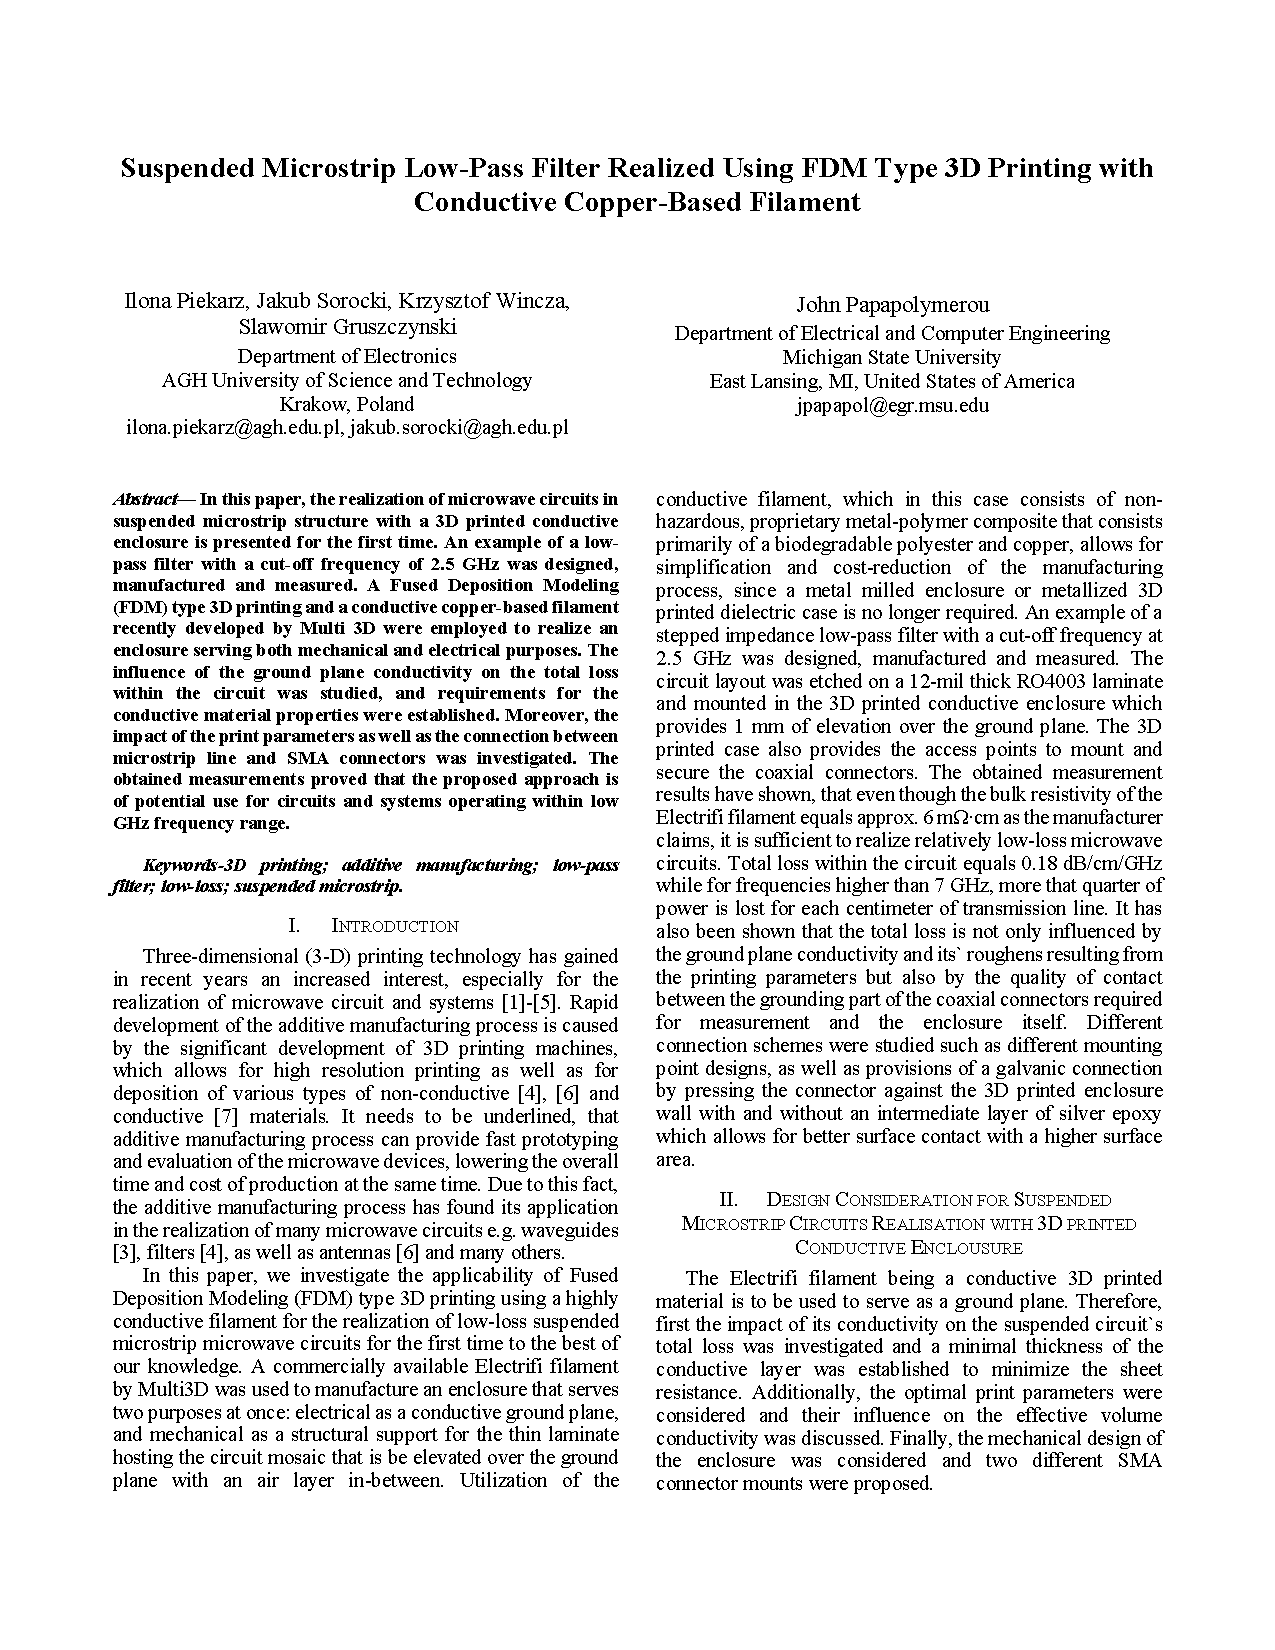
\includepdf[pages=-,addtotoc={1,section,1,Suspended microstrip low-pass filter realized using FDM type 3D printing with conductive copper-based filament,ectc_electr}, pagecommand={}, scale=.97]{chapter_5/ectc_electr.pdf}

\cleardoublepage

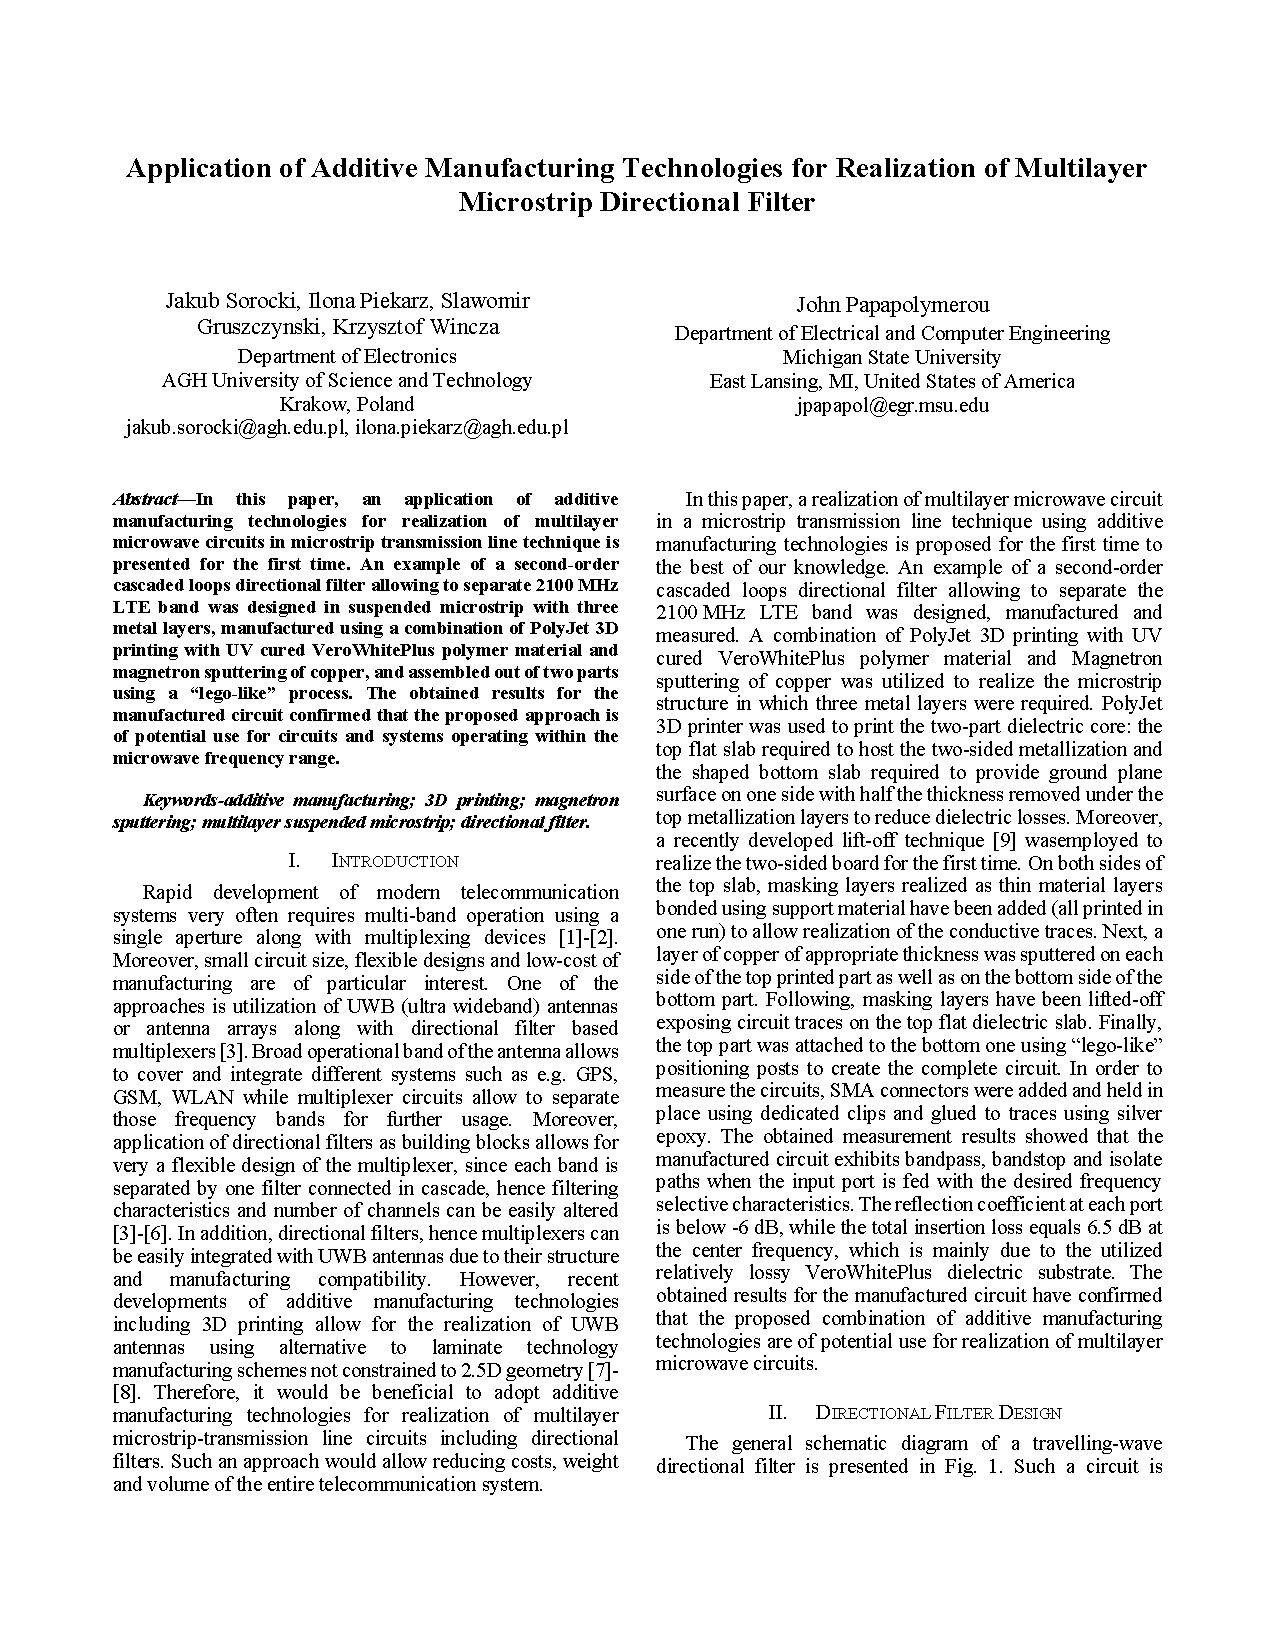
\includepdf[pages=-,addtotoc={1,section,1,Application of additive manufacturing technologies for realization of multilayer microstrip directional filter,ectc_df-poly}, pagecommand={}, scale=.97]{chapter_5/ectc_df-poly.pdf}

\cleardoublepage

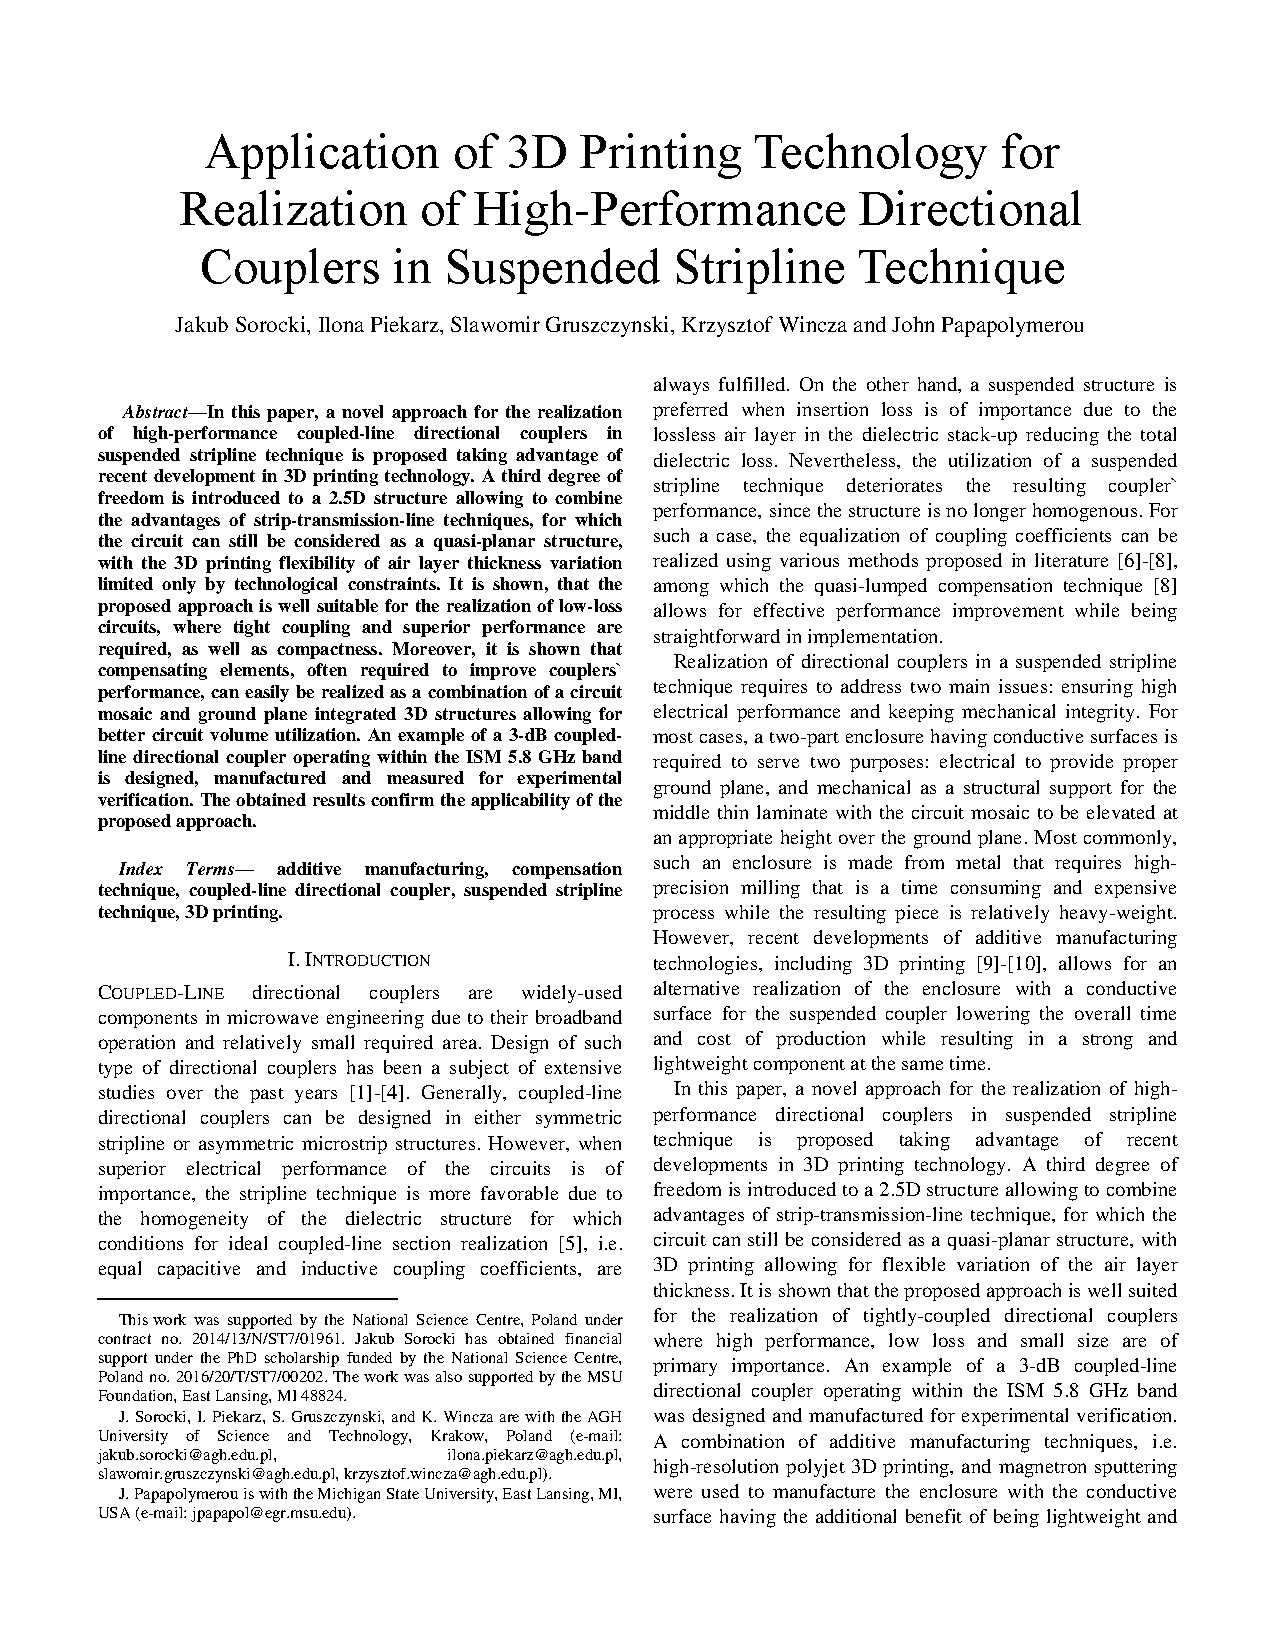
\includepdf[pages=-,addtotoc={1,section,1,Application of 3D printing technology for realization of high-performance directional couplers in suspended stripline technique,tmtt_right_left}, pagecommand={}, scale=.97]{chapter_5/polyjet_suspended_coupler.pdf}

\cleardoublepage
\chapter{Circuits` performance improvement by reducing internal power loss}\label{front}
%\addcontentsline{toc}{chapter}{Apendix}	% to be visible in TOC but unnuvered

\indent In this Chapter it is shown that power loss reduction allows to extend the functional range of a circuit on an example of a low-cost impedance tuner for push-pull transistor measurement. The usable range of realizable impedances is increased by replacing the core circuit from a larger and more lossy rat-race coupler to a six times smaller coupled-line coupler  to allow for measurement of power transistors featuring very low input/output impedance, which in addition requires shorter lengths of the tuning sliding loads. Such measurements are in many cases crucial for the design of high-power microwave amplifiers as in the developed high-power transceiver front-end where the proposed tuner was used to find  terminating impedances at the transistor`s input and output for the maximum power. The results of the conducted research have been a subject of a conference paper presented at \textit{Radio and Wireless Symposium RWS`16} under the auspices of \textit{Institute of Electrical and Electronics Engineers} and a technical report on the realization of \textit{RF Pulsed Power Amplifier} work package within \textit{Air traffic control system of the new generation ADS-B/MLAT} project granted by the National Centre for Research and Developement under the POIR program to Avionix Engineering Sp. z o. o., ID project number POIR.01.01.01-00-0169/15, which constitute the Chapter.
\\
\indent A low-cost impedance tuner is shown in Section \ref{rws_tuner} being well suitable for load-/source-pull transistor measurements. The proposed circuit consists of a 3-dB quadrature coupled-line directional coupler with tuning components realized as shorted microstrip line sections with appropriate sliding shorting elements, which allow to provide any desired impedance. The theoretical analysis of the proposed circuit has been performed and the principle of circuit’s behavior has been explained. An exemplary impedance tuner has been designed, manufactured and measured. The obtained measurement results showed the Voltage Standing Wave Ratio (VSWR) as high as 41:1 translating to a load impedance as low as $Z_{L}$ = 1.26 $\Omega $ proving usefulness and demonstrating the advantages of the presented approach.
\\
\indent Following, a custom power amplifier for the product components “Automatic dependent surveillance – broadcast (ADS-B) vehicle transponder” and “MODE-S interrogator” was of need. An RF power amplifier working in pulsed mode with minimum of 20 W peak output power for efficient Pulse-Position Modulation (PPM) amplification is designed and described in Section \ref{avionix_report} to be used as a part of the ADS-B vehicle transponder where small size and low power consumption are of importance. Moreover, the amplifier is integrated into a transceiver front-end module with a RX/TX switch for the operation with a single antenna. The developed module consist of an MMIC pre-amplifier module and an RF transistor based power amplifier. The utilized transistor was measured during the design process using source and load-pull technique with low-cost impedance tuners to allow for the determination of input and output terminating impedances that ensure maximum power amplification. Measurement results show compliance of the manufactured front-end with the design requirements.
% RF transisor NXP MRFE6VS25 on a short mount, VD = 40V, VG = 2.5V, Pin = 0 dBm + wzmacniacz + 30 dBm
%  1030 MHz bramka - stroik Z=2.52-j6.75 Ohm, Z=|0.905| -164.55deg
%  1030 MHz dren - stroik Z=5.98-j1.07 Ohm, Z=|0.786| -177.5deg
%  1090 MHz bramka - stroik Z=9.4-j3.9 Ohm, Z=|0.685| -170.7deg
%  1090 MHz dren - stroik Z=4.93-j2.78 Ohm, Z=|0.82| -177.3deg

\cleardoublepage

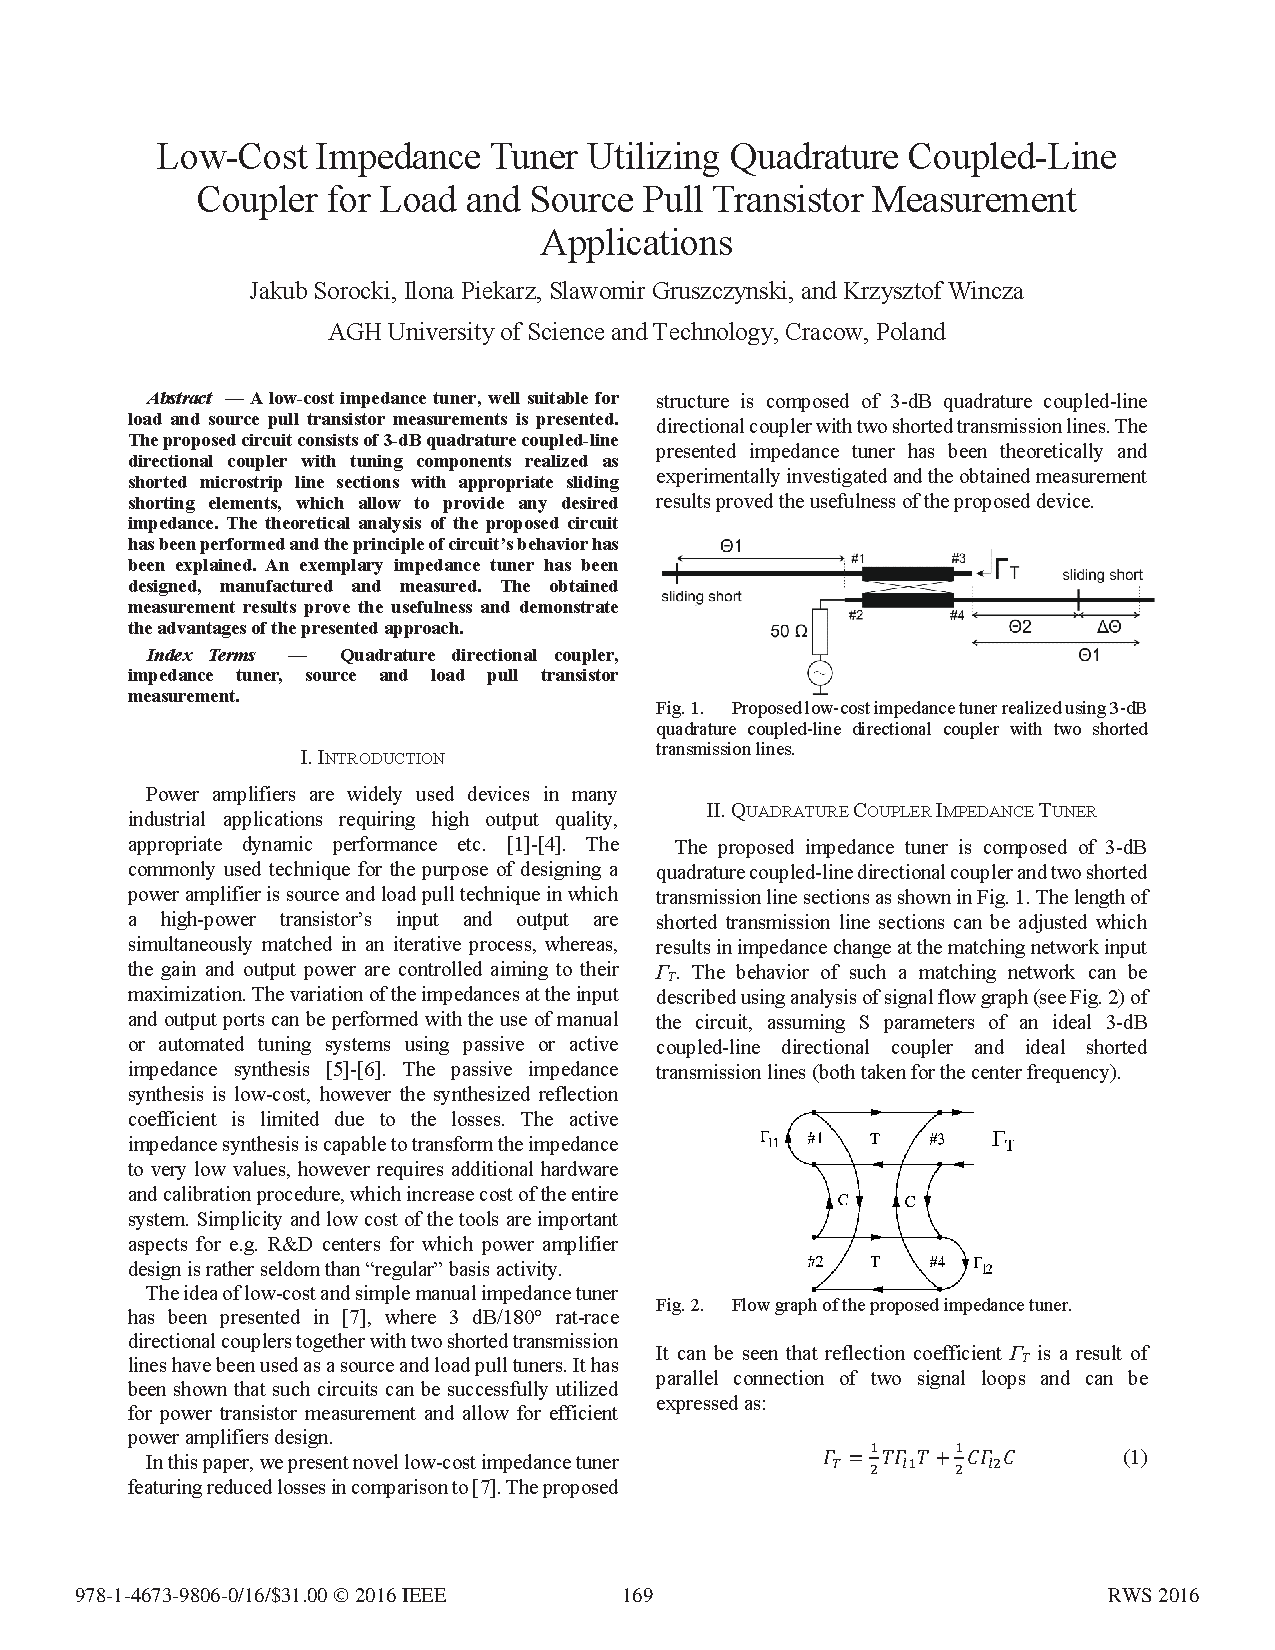
\includepdf[pages=-,addtotoc={1,section,1,Low-cost impedance tuner utilizing quadrature coupled-line coupler for load and source pull transistor measurement applications,rws_tuner}, pagecommand={}, scale=.97]{chapter_6/rws_tuner.pdf}

\cleardoublepage

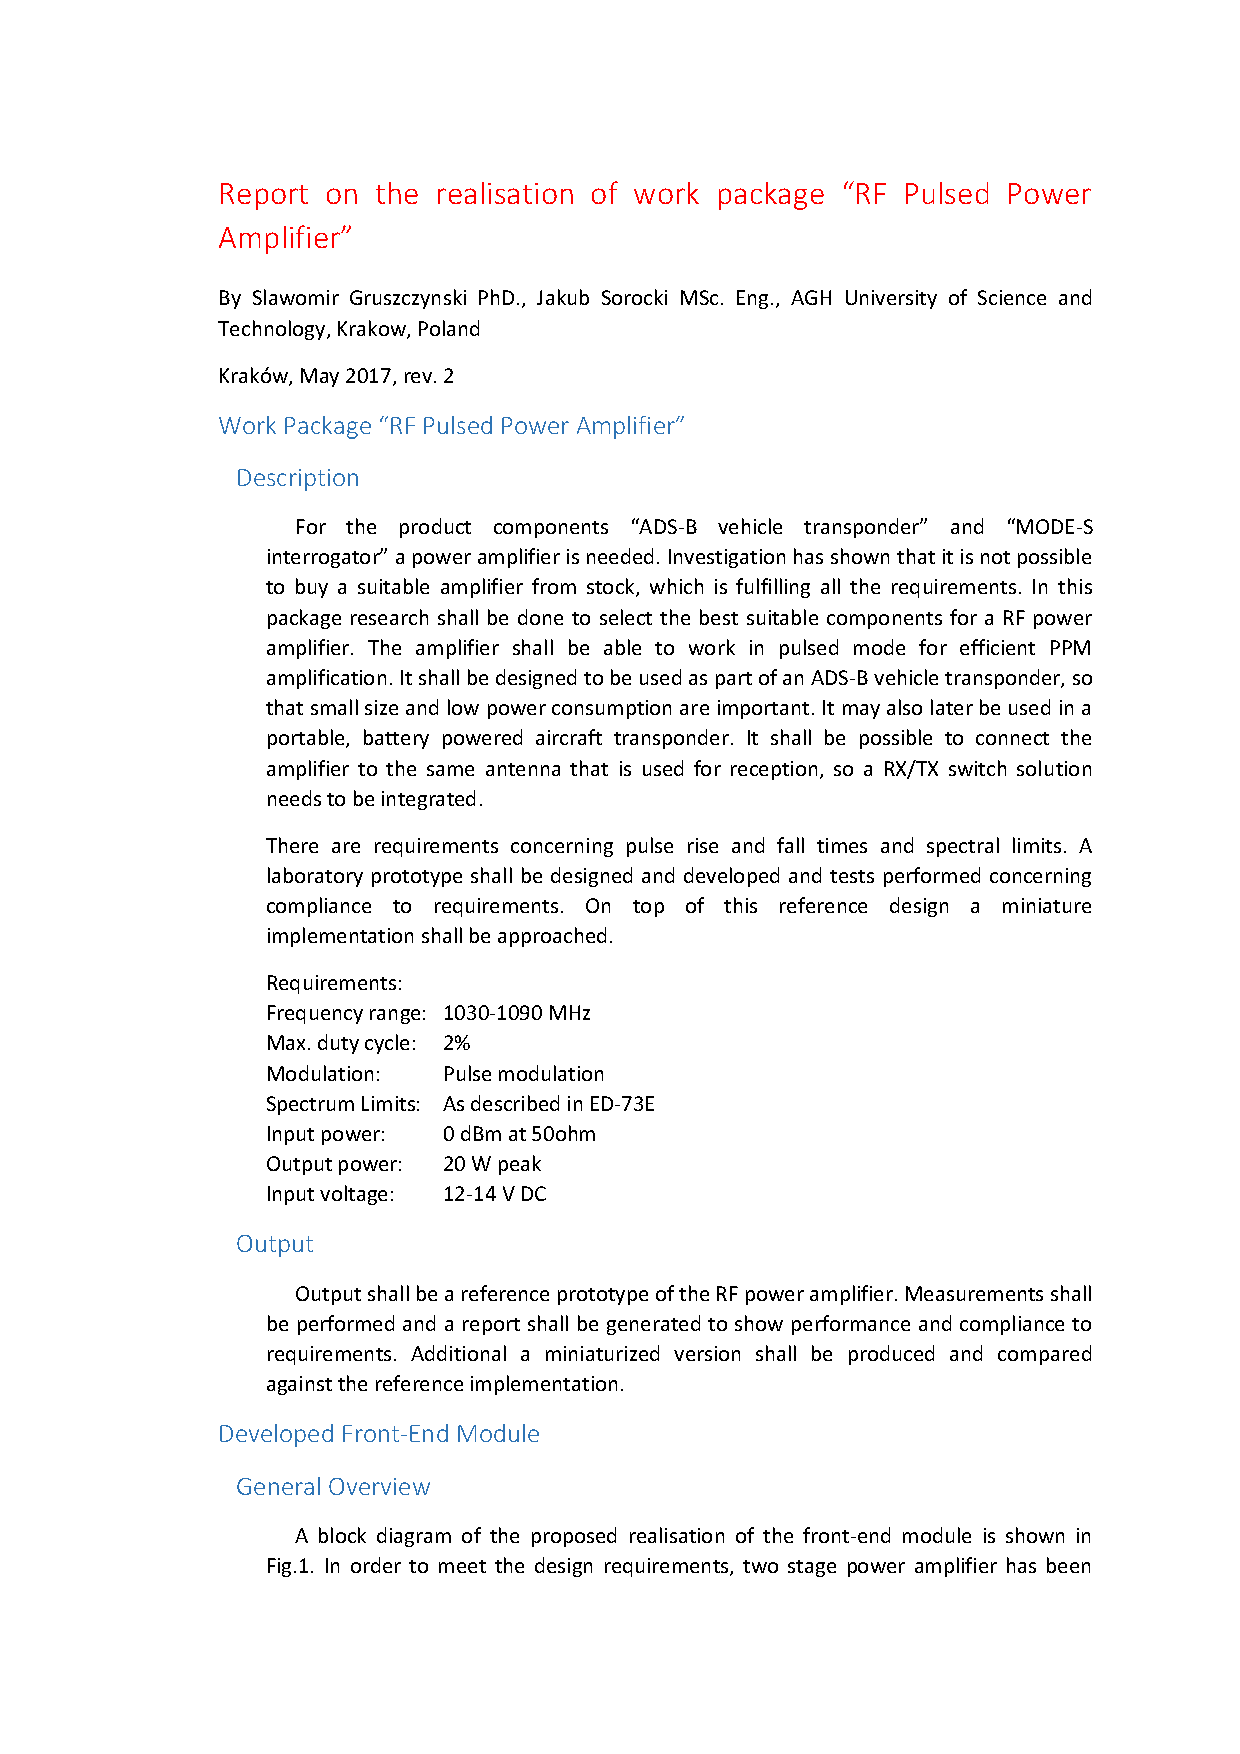
\includepdf[pages=-,addtotoc={1,section,1,Report on the realization of work package \textit{RF Pulsed Power
Amplifier} within the \textit{Air traffic control system of the new generation ADS-B/MLAT} project,avionix_report}, pagecommand={}, scale=.97]{chapter_6/avionix_report.pdf}

\cleardoublepage
\chapter{Summary}\label{summary}

\indent In this Thesis the realization of low-loss microwave circuits in strip transmission line technique was studied. As a result, the Author proposed several novel design methodologies, circuit topologies and realization schemes. The conducted theoretical studies were supported with experimental results on an example of numerous manufactured circuits. Within the scope of the Thesis, various approaches were considered and investigated with the focus on power loss reduction.
\\
\indent Circuit topologies and realization schemes being an alternative to the  classic solutions, were studied on an example of microwave filters to allow for obtaining a given functionality while featuring improved properties such as highly-selective frequency response, compact physical size or relatively low insertion loss. The periodic structures approach was considered and proven to be well suitable for the realization of filters for which a cascade connection of $n$ identical, electrically small unit cells of given properties is used.
\\
\indent Following, the Author investigated the influence of circuit topology and realization technique on the total power loss on an example of broadband pseudo-highpass microwave filters. It was shown that by replacement of relatively lossy lumped components with distributed type ones as well as by substitution of stripline/microstrip dielectric stack-up to suspended stripline/microstrip stack-up, a significant reduction of power loss can be achieved.
\\
\indent Moreover, in this Thesis design methodologies and circuit topologies focused on the performance improvement were studied to allow for power loss reduction on an example of directional filters and directional couplers. It was shown, that high-performance circuits can meet the design requirements while featuring shorter total electrical length or requiring less physical area, therefore, reducing total power loss.
\\
\indent Furthermore, the Author investigated the approach for power loss reduction within the system by the integration of functionalities within one circuit to reduce the number of components and by increasing level of functional blocks' integration. An example of division/summation networks in terms of power level and frequency spectrum, circuits with simultaneous power division and impedance transformation were shown for the application in compact multi-channel power amplifiers. Moreover, directional-filters-based frequency multiplexers have been proposed, where a high selectivity is obtained by the integration of both filter`s response and multiplexer`s topology properties.
\\
\indent Additionally, the Author considered the application of novel materials and manufacturing technologies for low-loss circuits` realization within microwave frequency range. It was shown that by enabling the 3\textsuperscript{rd} degree of structure's control, the design of compact high-performance circuits is possible as it was shown on an example of directional couplers. Moreover, aspects such as materials` conductivity, dielectric properties and manufacturing technologies have been investigated in terms of requirements for low-loss circuits` realization.
\\
\indent Finally, it was shown that the reduction of power loss allows to extend the circuit functionality on an example of a broad-range impedance tuner for source and load pull transistor measurements. The proposed tuner was proven to be useful for finding optimal terminating impedances for maximum power termination of high-power transistors by the design of an exemplary transceiver front-end.
\\
\indent The original achievements of the Author presented in this Thesis can be summarized as follows:

\begin{itemize}[nosep]
%\renewcommand{\labelitemi}{$\bullet$}
\item Development of compact unit cells composed of coupled and uncoupled transmission line sections allowing for bandpass filters` realization, published in \cite{tmtt_right_left}.
\item Development of a compact unit cell composed of transmission line sections allowing for bandstop filters' realization, published in \cite{mwcl_dcrlh}.
\item Development of pseudo-highpass filters composed of transmission line sections and lumped capacitor unit cells, published in \cite{jemwa_pseudo-highpass}.
\item Development of loss-reduced pseudo-highpass filters composed of transmission line sections and lumped capacitor unit cells, published in \cite{mms_low-loss_wideband}.
\item Development of loss-reduced pseudo-highpass filters composed of unit cells constructed of coupled and uncoupled transmission line sections, published in \cite{mikon_low-loss_distributed}.
\item Development of miniaturized traveling wave directional filters, published in \cite{isap_miniaturized_DF}.
\item Development of traveling wave directional filters with additional, easily controllable transmission zeroes created by the appropriate cascading two identical filters, published in \cite{mikon_cascaded_DF}.
\item Development of low-loss directional filters composed of two differential bandstop filters featuring improved isolation bandwidth, published in \cite{mwcl_band_reject}.
\item Development of traveling-wave directional filters with additional, easily controllable transmission zeroes created by the introduction of loose cross coupling, published in \cite{tmtt_crosscoupled_DF}.
\item Development of the design approach for frequency multiplexers where an increased selectivity of each channel is obtained by the appropriate design of asymmetric directional filters and taking advantage of multiplexer`s topology, published in \cite{mwcl_cascaded_multipex}.
\item Development of an impedance transforming directional coupler with a high impedance transformation ratio, published in \cite{jmwt_imp_tranforming}.
\item Development of a broadband directional coupler composed of loosely coupled single-section directional couplers in tandem configuration, published in \cite{mwcl_tandem}.
%\item Development of an impedance transforming balance-to-unbalance signal converting circuit, published in \cite{jiee_imp_tranf_balun}.
\item Theoretical investigation, confirmed with experimental results on the application of FDM type 3D printing with conductive filaments for the realization of low-loss microwave circuits in suspended microstrip technique, published in \cite{iceese_3D_graphene} and \cite{ectc_electrify}.
\item Development of the realization technique of multilayers microstrip circutis using a combination of additive manufacturing technique, published in \cite{ectc_df}.
\item Development of design methodology with enabled 3\textsuperscript{rd} degree of structure control using 3D printing for the realization of high-performance directional couplers in suspended stripline, published in \cite{polyjet_susp_coupler}.
\item Development of a low-cost impedance tuner with realizable ratio of VWSR as high as 41:1 for load and source pull transistor measurement, published in \cite{rws_imp_tuner}.
\item Development of a high-power RF front-end for ADS-B vehicle transponder and MODE-S interrogator with 20 W peak output power amplifier, described in \cite{avionix_report}.
\end{itemize}

\indent In the view of the above listed achievements being a result of investigatig the presented approaches for power loss reduction it can be concluded, that the goals stated in \hyperref[intro:goal]{Introduction} have been achieved. Various design techniques, circuit topologies and realization schemes have been investigated proving that filters (goal I) and power division/summation circuits such as directional couplers and frequency multiplexers (goal II) can be realized in strip transmission line technique featuring low power loss and high performance. Finally, an exemplary high-power RF front-end was developed (goal III).
\\
\indent The Author believes that the research results presented in the Thesis focused on power loss minimization of circuits realized in strip transmission line technique will contribute to the development of microwave theory and techniques and will be useful for further development of highly integrated functional blocks of wireless telecommunication systems. The replacement of currently used combination of all-metal waveguides and PCB technology with one uniform realization technique will allow for more efficient utilization of the system`s physical volume and better integration of particular building blocks leading to fulfillment of the above stated demands for transmitting and receiving capabilities.
\\
\indent Further research efforts will be focused on the application of 3D printing technologies and novel materials for the realization of low-loss strip transmission line circuits with enabled third dimension of circuit control opening new directions of circuits` and systems` development. The preliminary results presented e.g. in \cite{iceese_3D_graphene}, \cite{ectc_electrify}, \cite{ectc_df}, \cite{polyjet_susp_coupler}, \cite{apwc_absorber}, \cite{iceaa_magnetic} have shown the potential of such an approach. However, there are challenges that needs to be addressed in order to increase the applicability of the 3D printing technology.
\\
\indent Another promising direction of further research can be found in the design and manufacturing of very high frequency circuits where waveguide technique is replaced with strip transmission line technique. It has been shown in \cite{tmtt_aerosol} and \cite{eumw_aerosol} that the application of aerosol jet 3D printing technology in combination with conductive inks and very low loss dielectric inks has a potential for the realization of mm-wave circuits. However, further development is required in terms of materials` and manufacturing processes` optimization.

\cleardoublepage

%\fancyhead[L]{\slshape{\small \leftmark}}		% nazwa rozdzia�u w nag��wku
\fancyhead[LO]{\slshape{\small \leftmark}}
\fancyhead[RO]{\bfseries \thepage}
\fancyhead[RE]{\slshape{\small \leftmark}}
\fancyhead[LE]{\bfseries \thepage}

%--- back matter ---
% bibliography, authors info

%\fancyhead[L]{\slshape{\small \leftmark}}
%\fancyhead[L]{\slshape{\small Bibliography}}		% zmiana nag��wka
\fancyhead[LO]{\slshape{\small Bibliography}}
\fancyhead[RO]{\bfseries \thepage}
\fancyhead[RE]{\slshape{\small Bibliography}}
\fancyhead[LE]{\bfseries \thepage}

\bibliographystyle{IEEEtran_no_dash}	%IEEE sortowanie kolejnoscia wystapnienia
\bibliography{references_main,references_misc} % for multiple file bibliography  notsubtype=inet
%\bibliography{references_main}
%\bibliographystylemisc{IEEEtran_no_dash}
%\nobibliography{references_misc}
\addcontentsline{toc}{chapter}{Bibliography}

%\fancyhead[L]{\slshape{\small Author's Achievements}}		% zmiana nag��wka
\fancyhead[LO]{\slshape{\small Author's Achievements}}
\fancyhead[RO]{\bfseries \thepage}
\fancyhead[RE]{\slshape{\small Author's Achievements}}
\fancyhead[LE]{\bfseries \thepage}
\chapter*{Author's Achievements}\label{chapter_author_biblio}
\addcontentsline{toc}{chapter}{Author's Achievements}


\noindent \textbf{Journal papers focused directly on the dissertation`s subject}:
\begin{itemize}[nosep]
\item \bibentry{polyjet_susp_coupler}
\item \bibentry{mwcl_cascaded_multipex}
\item \bibentry{tmtt_crosscoupled_DF}
\item \bibentry{mwcl_band_reject}
\item \bibentry{jmwt_imp_tranforming}
\item \bibentry{jiee_imp_tranf_balun}
\item \bibentry{mwcl_dcrlh}
\item \bibentry{jemwa_pseudo-highpass}
\item \bibentry{tmtt_right_left}
\item \bibentry{mwcl_tandem}
\end{itemize}
\vspace*{1cm} %\vfill

\noindent \textbf{Journal papers not related to the dissertation's subject}:
\begin{itemize}[nosep]
%\item \bibentry{tmtt_aerosol}
\item I. Piekarz, J. Sorocki, M. T. Craton, K. Wincza, S. Gruszczynski, and J. Papapolymerou,
“Applications of aerosol jet 3D printing with conductive and non-conductive inks for the realization of mm-wave circuits,” \textit{in preparation}, 2018
%\item \bibentry{mwcl_three_section_diff}
\item I. Piekarz, J. Sorocki, K. Janisz, K. Wincza, and S. Gruszczynski, “Wideband three-section
symmetrical coupled-line directional coupler operating in differential mode,” submitted to \textit{IEEE Microwave and Wireless Components Letters}, 2018
%\item \bibentry{mwcl_tandem_three}
%\item \bibentry{sensors_two_wire}
\item I. Piekarz, J. Sorocki, K. Wincza, and S. Gruszczynski, “Liquids permittivity measurement using two-wire transmission line sensor,” submitted to \textit{IEEE Sensors Journal}, 2018
%\item \bibentry{tie_vector}
\item K. Staszek, I. Piekarz, J. Sorocki, S. Koryciak, K. Wincza, and S. Gruszczynski, “Low-cost
microwave vector system for liquid properties monitoring,” \textit{IEEE Transactions on Industrial Electronics}, vol. 65, no. 2, pp. 1665–1674, Feb. 2018
%\item \bibentry{tmtt_coupled_sensor}
\item I. Piekarz, J. Sorocki, K. Wincza, and S. Gruszczynski, “Microwave sensors for dielectric samples measurement based on coupled-line section,” \textit{IEEE Transactions on Microwave Theory and Techniqes}, vol. 65, no. 5, pp. 1615–1631, May 2017
%\item \bibentry{jemwa_leaky}
\item I. Slomian, J. Sorocki, S. Gruszczynski, and K. Wincza, “Composite right-left handed leaky-wave antenna with adjustable radiation bandwidth,” \textit{Journal of ElectromagneticWaves and Applications}, vol. 30, no. 8, pp. 1054–1063, 2016
%\item \bibentry{jiee_imp_tranf_balun}
\item J. Sorocki, I. Piekarz, P. Kaminski, K. Wincza, and S. Gruszczynski, “Broadband balun circuits composed of impedance transforming directional couplers and LH transmission-line sections,” \textit{International Journal of Microwave and Wireless Technologies}, vol. 6, no. 3, pp. 147–150, 2016
%\item \bibentry{ijmwt_two_section}
\item J. Sorocki, K. Staszek, I. Piekarz, K. Wincza, and S. Gruszczynski, “Application of RH and LH sections for reduction of coupling coefficients in two-section asymmetric directional couplers,” \textit{International Journal of Microwave and Wireless Technologies}, vol. 8, pp. 559–565, May 2016
%\item \bibentry{sensors_coupled}
\item I. Piekarz, J. Sorocki, K.Wincza, and S. Gruszczynski, “Coupled-line sensor with marchand balun as RF system for dielectric sample detection,” \textit{IEEE Sensors Journal}, vol. 16, no. 1, pp. 88–96, Jan. 2016
%\item \bibentry{mwcl_balun}
\item I. Piekarz, J. Sorocki, S. Gruszczynski, and K. Wincza, “Input match and output balance
improvement of marchand balun with connecting line,” \textit{IEEE Microwave and Wireless
Components Letters}, vol. 24, no. 10, pp. 683–685, Oct. 2014
%\item \bibentry{rfmcae_modelling_coupled}
\item I. Piekarz, J. Sorocki, S. Gruszczynski, and K. Wincza, “Modeling and performance improvement of folded coupled lines in miniaturized quasi-lumped directional couplers,” \textit{International Journal of RF and Microwave Computer-Aided Engineering}, vol. 25, no. 1, pp. 1–9, Jan. 2015
%\item \bibentry{rfmcae_magic-T}
\item J. Sorocki, I. Piekarz, K. Wincza, and S. Gruszczynski, “Broadband magic-Ts with the use
of coupled-line directional couplers and left-handed transmission line sections,” \textit{International Journal of RF and Microwave Computer-Aided Engineering}, vol. 24, no. 4, pp. 513–521, Jul. 2014
%\item \bibentry{map_reduced_couppling}
\item J. Sorocki, K. Staszek, I. Piekarz, K. Wincza, and S. Gruszczynski, “Directional couplers
with reduced coupling requirements as a connection of coupled-line sections and left-handed
transmission lines,” \textit{IET Microwaves, Antennas and Propagation}, vol. 8, no. 8, pp. 580–588, Jun. 2014
%\item \bibentry{rfmcae_rat-race}
\item J. Sorocki, I. Piekarz, K. Wincza, and S. Gruszczynski, “Bandwidth improvement of rat-race
couplers having left-handed transmission-line sections,” \textit{International Journal of RF and
Microwave Computer-Aided Engineering}, vol. 24, no. 3, pp. 341–347, May 2014
%\item \bibentry{motl_ltcc}
\item I. Piekarz, J. Sorocki, K. Wincza, S. Gruszczynski, J. Muller, and T. Welker, “Miniaturized
quasi-lumped coupled-line single-section directional coupler designed in multilayer LTCC
technology,” \textit{Microwave and Optical Technology Letters}, vol. 55, no. 6, pp. 1401–1405, Jun. 2013
\end{itemize}
\vspace*{1cm} %\vfill

\noindent \textbf{Conference communicates focused directly on the dissertation's subject}:
\begin{itemize}[nosep]
\item \bibentry{mikon_low-loss_distributed}
\item \bibentry{ectc_electrify}
\item \bibentry{ectc_df}
\item \bibentry{iceese_3D_graphene}
\item \bibentry{mms_low-loss_wideband}
\item \bibentry{rws_imp_tuner}
\item \bibentry{mikon_cascaded_DF}
\item \bibentry{isap_miniaturized_DF}
\end{itemize}
\vspace*{1cm} %\vfill

\noindent \textbf{Conference communicates not related to the dissertation's subject}:
\begin{itemize}[nosep]
%\item \bibentry{eumw_aerosol}
\item M. T. Craton, J. Sorocki, I. Piekarz, S. Gruszczynski, K. Wincza, and J. Papapolymerou,
“Realization of fully 3D printed W-band bandpass filters using aerosol jet printing technology,”
submitted to \textit{European Microwave Week (EuMW 2018)}, Madrid, Spain, Sep. 2018
%\item \bibentry{mikon_coupled_liquid}
\item \bibentry{apwc_absorber}
\item \bibentry{iceaa_magnetic}
\item I. Slomian, J. Sorocki, I. Piekarz, K. Wincza, and S. Gruszczynski, “Aperture-coupled microstrip antenna integrated with PET-G dielectric lens,” in \textit{International Conference on Electromagnetics in Advanced Applications (ICEAA 2018)}, Cartagena de Indias, Colombia, Sep. 2018.
\item I. Piekarz, J. Sorocki, K. Wincza, and S. Gruszczynski, “Coupled-line sensor setup with liquids and solids permittivity sensing capability developed with the use of 3D printing technology,” in \textit{International Conference on Microwave, Radar and Wireless Communications (MIKON 2018)}, Poznan, Poland, May 2018
%\item \bibentry{iceese_multi}
\item I. Piekarz, J. Sorocki, K. Wincza, and S. Gruszczynski, “Multi-coupled-line microwave sensors for dielectric sample permittivity change detection,” in \textit{International Conference on Electrical, Electronics and System Engineering (ICEESE 2017)}, Kanazawa, Japan, Nov. 2017, pp. 48–51
%\item \bibentry{comite_antenna}
\item J. Sorocki, I. Piekarz, S. Gruszczynski, and K. Wincza, “Approach to the design of wideband
antenna arrays with reduced coupling between elements,” in \textit{Conference on Microwave Techniques
(COMITE 2017)}, Brno, Czech Republik, Apr. 2017
%\item \bibentry{comite_sensor}
\item I. Piekarz, J. Sorocki, K. Wincza, and S. Gruszczynski, “Low-cost planar coupled-line sensor for permittivity measurement of low-loss dielectric materials in a wide frequency range,” in \textit{Conference on Microwave Techniques (COMITE 2017)}, Brno, Czech Republik, Apr. 2017
%\item \bibentry{comite_system}
\item I. Piekarz, K. Janisz, J. Sorocki, K. Wincza, and S. Gruszczynski, “Two-port measurement
system with coupled-line sensor for detection of material permittivity change,” in \textit{Conference on Microwave Techniques (COMITE 2017)}, Brno, Czech Republik, Apr. 2017
%\item \bibentry{rws_rat}
\item I. Piekarz, J. Sorocki, K.Wincza, and S. Gruszczynski, “Rat-race directional couplers operating in differential mode,” in \textit{Radio and Wireless Symposium (RWS 2017)}, Phoenix, AZ, USA, Jan. 2017
%\item \bibentry{msmw_compact}
\item J. Sorocki, I. Piekarz, S. Gruszczynski, and K. Wincza, “Compact microstrip coupled-line
directional coupler realized in thick-film technology,” in \textit{International Kharkiv Symposium on Physics and Engineering of Microwaves, Millimeter and Submillimeter Waves (MSMW 2016)}, Kharkiv, Ukraine, Jun. 2016
%\item \bibentry{msmw_differentialy}
\item J. Sorocki, I. Piekarz, K. Wincza, and S. Gruszczynski, “Differentialy excited coupled-line
sensor for small dielectric samples detection,” in \textit{International Kharkiv Symposium on Physics and Engineering of Microwaves, Millimeter and Submillimeter Waves (MSMW 2016)}, Kharkiv,
Ukraine, Jun. 2016
%\item \bibentry{msmw_miniaturized}
\item J. Sorocki, I. Piekarz, K. Wincza, and S. Gruszczynski, “Miniaturized microstrip marchand balun and coupled-line section as microwave sensor for dielectric material detection,” in \textit{International Kharkiv Symposium on Physics and Engineering of Microwaves, Millimeter and Submillimeter Waves (MSMW 2016)}, Kharkiv, Ukraine, Jun. 2016
%\item \bibentry{msmw_sensitivity}
\item Piekarz, J. Sorocki, S. Gruszczynski, and K. Wincza, “Sensitivity investigation of coupled-line microwave sensor on dielectric Material-Under-Test,” in \textit{International Kharkiv Symposium on Physics and Engineering of Microwaves, Millimeter and Submillimeter Waves (MSMW 2016)}, Kharkiv, Ukraine, Jun. 2016
%\item \bibentry{msmw_simplified}
\item I. Piekarz, J. Sorocki, K.Wincza, and S. Gruszczynski, “Simplified three-strip coupled-line section as microwave sensor for dielectric materials measurement,” in \textit{International Kharkiv Symposium on Physics and Engineering of Microwaves, Millimeter and Submillimeter Waves (MSMW 2016)}, Kharkiv, Ukraine, Jun. 2016
%\item \bibentry{msmw_calibration}
\item I. Piekarz, J. Sorocki, K. Wincza, and S. Gruszczynski, “Calibration method of microwave
measurement system for dielectric samples detection,” in\textit{ International Kharkiv Symposium on Physics and Engineering of Microwaves, Millimeter and Submillimeter Waves (MSMW 2016)},
Kharkiv, Ukraine, Jun. 2016
%\item \bibentry{mikon_compensated}
\item I. Piekarz, J. Sorocki, K. Wincza, and S. Gruszczynski, “Miniaturized compensated quasi-lumped wideband Marchand balun,” in \textit{International Conference on Microwave, Radar and Wireless Communications (MIKON 2016)}, Krakow, Poland, May 2016
%\item \bibentry{rws_effective}
\item I. Piekarz, J. Sorocki, K. Wincza, and S. Gruszczynski, “Effective permittivity measurement with the use of coupled-line section sensor,” in \textit{Radio and Wireless Symposium (RWS 2016)}, Austin, TX, United States of America, Jan. 2016
%\item \bibentry{isap_wideband}
\item I. Piekarz, J. Sorocki, K. Wincza, and S. Gruszczynski, “Wideband marchand balun and bow-tie antenna for sensor applications,” in \textit{International Symposium on Antennas and Propagation (ISAP 2015)}, Hobart, Australia, Nov. 2015
%\item \bibentry{isap_leaky}
\item S. Gruszczynski, A. Rydosz, J. Sorocki, I. Slomian, P. Kaminski, and K. Wincza, “Leaky-wave
antenna in multilayer structure for sensor applications,” in \textit{International Symposium on Antennas and Propagation (ISAP 2015}), Hobart, Australia, Nov. 2015
%\item \bibentry{wamicon_slot}
\item J. Sorocki, I. Piekarz, I. Slomian, K. Wincza, and S. Gruszczynski, “Approach to the design
of slot-coupled-line directional couplers,” in \textit{Wireless and Microwave Technology Conference (WAMICON 2015)}, Cocoa Beach, FL, United States of America, Apr. 2015
%\item \bibentry{wamicon_marchand}
\item I. Piekarz, J. Sorocki, I. Slomian, K. Wincza, and S. Gruszczynski, “Compact single-layer
microstrip marchand type balun,” in \textit{Wireless and Microwave Technology Conference (WAMICON
2015)}, Cocoa Beach, FL, United States of America, Apr. 2015
%\item \bibentry{mms_magicT}
\item J. Sorocki, I. Piekarz, I. Slomian, K. Staszek, K. Wincza, and S. Gruszczynski,
“Bandwidth-enhanced single-layer 3-dB tandem directional coupler as magic-T network,” in
\textit{Mediterranean Microwave Symposium (MMS 2014)}, Marrakech, Morocco, Dec. 2014
%\item \bibentry{mms_marchand}
\item I. Piekarz, J. Sorocki, I. Slomian, K. Staszek, K. Wincza, and S. Gruszczynski, “Marchand
balun with connecting segment designed with the use of multi-technique compensation,” in
\textit{Mediterranean Microwave Symposium (MMS 2014)}, Marrakech, Morocco, Dec. 2014
%\item \bibentry{mms_lattice}
\item I. Slomian, K. Staszek, I. Piekarz, J. Sorocki, K. Wincza, and S. Gruszczynski, “Dual polarized two-port antenna lattice,” in \textit{Mediterranean Microwave Symposium (MMS 2014)}, Marrakech, Morocco, Dec. 2014
%\item \bibentry{isap_leaky_meta}
\item S. Gruszczynski, A. Rydosz, J. Sorocki, I. Slomian, and K. Wincza, “Leaky-wave antenna
with modified metamaterial unit cell for narrowing beam steering bandwidth,” in \textit{International Symposium on Antennas and Propagation (ISAP 2014)}, Kaohsiung, Taiwan, Dec. 2014
%\item \bibentry{mikon_magicT}
\item J. Sorocki, I. Piekarz, I. Slomian, S. Gruszczynski, and K. Wincza, “Single-layer coupled-line magic-ts utilizing left-handed transmission line sections,” in \textit{International Conference on Microwave, Radar and Wireless Communications (MIKON 2014}), Gdansk, Poland, May 2014
%\item \bibentry{mikon_array24}
\item I. Slomian, P. Kaminski, J. Sorocki, I. Piekarz, K. Wincza, and S. Gruszczynski, “Multi-beam and multi-range antenna array for 24 GHz radar applications,” in \textit{International Conference on Microwave, Radar and Wireless Communications (MIKON 2014)}, Gdansk, Poland, May 2014
%\item \bibentry{crimico_four}
\item I. Piekarz, J. Sorocki, I. Slomian, M. Sloma, P. Kaminski, K. Wincza, and S. Gruszczynski,
“Miniaturized coupled-line directional coupler designed with the use of photoimageable thick-film
technology,” in \textit{International Crimean Conference Microwave and Telecommunication Technology (CriMiCo 2013), Sevastopo}l, Ukraine, Sep. 2013
%\item \bibentry{crimico_antenna}
\item P. Sanz, I. Slomian, I. Piekarz, J. Sorocki, P. Kaminski, K. Wincza, and S. Gruszczynski,
“Four-beam antena array for 24 GHz applications fed by 4x4 Butler matrix,” in \textit{International Crimean Conference Microwave and Telecommunication Technology (CriMiCo 2013)}, Sevastopol,
Ukraine, Sep. 2013
%\item \bibentry{imoc_antenna}
\item I. Slomian, J. Sorocki, P. Kaminski, A. Rydosz, K. Wincza, and S. Gruszczynski, “Broadband 4 x 4 microstrip antenna array utilizing slot-coupled power dividers,” in \textit{International Microwave and Optoelectronics Conference (IMOC 2013)}, Rio de Janeiro, Brasil, Aug. 2013
%\item \bibentry{telfor_asymmetric}
\item I. Piekarz and J. Sorocki, “Asymmetric coupled-line single-section directional coupler with
equalized inductive and capacitive coupling coefficients,” in \textit{Telecommunications Forum (TELFOR 2012)}, Belgrade, Serbia, Nov. 2012
%\item \bibentry{telfor_ltcc}
\item I. Piekarz, J. Sorocki, K. Wincza, and S. Gruszczynski, “Meandered coupled-line single-section directional coupler utilizing multilayer LTCC technology,” in \textit{Telecommunications Forum (TELFOR 2012)}, Belgrade, Serbia, Nov. 2012
\end{itemize}
\vspace*{1cm} %\vfill

\noindent \textbf{Leadership of research projects}:
\begin{itemize}[nosep]
\item Research project awarded by the National Science Centre under \textit{Etiuda} 4 program, entitled "Low-loss microwave circuits in strip transmission line technique. Analysis, design and experimental investigations". ID project number 2016/20/T/ST7/00202. Project granted for 2016--2018.
\item Research project awarded by the National Science Centre under \textit{Preludium} 7 program, entitled "Investigation on high-performance low-loss microwave directional filters for application in high-power systems". ID project number 2014/13/N/ST7/01961. Project granted for 2015--2018.
\end{itemize}
\vspace*{1cm} %\vfill

\noindent \textbf{Participation in research projects}:
\begin{itemize}[nosep]
\item Research Project granted by the National Centre for Research and Developement under the \textit{POIR} program, entitled "The use of tropospheric communication to increase the range of unmanned aerial vehicles - BSP" -- investigator. ID project~number POIR.01.01.01-00-0070/17. Project~granted for 2017--2019.
\item Research Project granted by the National Centre for Research and Developement under the \textit{Lider} program, entitled "Sensor nanostructures for use in portable breath analyzers" -- investigator. ID project~number LIDER/252/L-6/NCBR/2015. Project~granted for 2016--2019.
\item Research Project awarded by the National Centre for Research and Developement under the \textit{POIR} program, entitled "Air traffic control system of the new generation ADS-B / MLAT" -- investigator. ID project~number POIR.01.01.01-00-0169/15. Project~granted for 2016--2017.
\item Research Project granted by the Ministry of Science and Higher Education under the \textit{Iuventus Plus} Program (second edition), entitled, "Investigations on realization of low-loss passive microwave power division/summation circuits for applications in high-power microwave amplifiers" -- investigator. ID project number 0510/IP2/2015/73. Project granted for 2015--2019.
\item Research Project granted by the National Science Centre under the \textit{Sonata Bis} Program, entitled "Research on the transmission lines having negative phase velocity and their application to novel microwave circuits" -- investigator. ID project~number 2011/01/D/ST7/00789. Project~granted for 2011--2015.
\item Research Project granted by the Ministry of Science and Higher Education, entitled, "Miniaturized microwave broadband directional couplers designed with the use of quasi-lumped technique" -- investigator. ID project number 4999/B/T02/2011/40. Project granted for 2011--2013.
\item Research Project granted by the Ministry of Science and Higher Education under the \textit{Iuventus Plus} Program (second edition), entitled, "Broadband microwave directional couplers realized in structures having decreased available coupling coefficient -- synthesis methods, design and application to novel microwave electronics" -- investigator. ID project number 0604/IP2/2011/71. Project granted for 2011--2015.
\item Research Project granted by the National Centre for Research and Developement under the \textit{Lider} program, entitled "Miniature integrated radar devices for industrial applications and anti-collision radars" -- investigator. ID project~number 4999/B/T02/2011/40. Project~granted for 2012--2013.
\end{itemize}
\vspace*{1cm} %\vfill

\noindent \textbf{Research visits, internships, training courses}:
\begin{itemize}[nosep]
\item 2017.05-11 - Michigan State University, East Lansing, MI, United States of America – half-year research visit within NCN Etiuda program, cooperation with prof. I. Papapolimerou on the design and manufacturing of microwave circuits using additive 3D manufacturing technologies.
\item 2015.08 - Wageningen University, Wageningen, Netherlands – 2-week soft-skills and entrepreneurship course within ‘Transformation.doc’ organized by the Polish Ministry of Science and Higher Education for Young Scientists.
\item 2012-2013 - AGH University of Science and Technology, Krakow, Poland – Research Assistant internship in High Frequency Electronics and Microwave Technique Research Group under prof. S. Gruszczynski supervision.
\item 2012.04-0.9 - Ilmenau University of Technology, Ilmenau, Germany – half-year stay within LLP EASMUS student exchange program, cooperation with prof. J. Müeller on the design and manufacturing of microwave circuits in LTCC (Low Temperature Co fired Ceramics) technology.
\end{itemize}
\vspace*{1cm} %\vfill

\noindent \textbf{Active participation in scientific events}:
\begin{itemize}[nosep]
\item 68\textsuperscript{th} IEEE Electronic Components and Technology Conference ECTC'18, 29 May - 01 Jun. 2018, San Diego, CA, USA.
\item 22\textsuperscript{nd} International Conference on Microwaves, Radar, and Wireless Communications MIKON'18, 15-17 May 2018, Poznan, Poland.
\item 3\textsuperscript{rd} International Conference on Electrical, Electronics and System Engineering ICEESE'17, 09-10 Nov. 2017, Kanazawa, Japan.
\item Microwave and Radio Electronics Week MAREW'17 (18\textsuperscript{th} Conference on Microwave Techniques COMITE'17), 19-21 Apr. 2018, Brno, Czech Republic.
\item 11\textsuperscript{th} IEEE Radio and Wireless Week RWW'17, 15-18 Jan. 2017, Phoenix, AZ, USA. %11
\item 9\textsuperscript{th} International Kharkiv Symposium on Physics and Engineering of Microwaves, Millimeter and Submillimeter Waves MSMW'16, 20-24 Jun. 2016, Kharkiv, Ukraine.
\item XXXVIIIth IEEE-SPIE Joint Symposium Wilga 2016, 30 May. – 6 Jun. 2016, Wilga, Poland.
\item 21\textsuperscript{th} International Conference on Microwave, Radar and Wireless Communications MIKON'16, 9-11 May 2016, Krakow, Poland.
\item 10\textsuperscript{th} IEEE Radio and Wireless Week RWW'16, 24-27 Jan. 2016, Austin, TX, USA. %10
\item International Symposium on Antennas and Propagation ISAP'15, 9-12 Nov. 2015, Hobart, Tasmania, Australia.
\item 16\textsuperscript{th} IEEE MTT-S Wireless and Microwave Technology Conference WAMICON'15, 13-15 Apr. 2015, Cocoa Beach, FL, USA.
\item 14\textsuperscript{th} Mediterranean Microwave Symposium MMS'14, 12-14 Dec. 2014, Marrakech, Morocco.
\item 24\textsuperscript{th} International Travelling Summer School on Microwaves and Lightwaves, 5-11 Jul. 2014, Copenhagen, Denmark.
\item 20\textsuperscript{th} International Conference on Microwaves, Radar, and Wireless Communications MIKON'14, 16-18 Jun. 2014, Gdansk, Poland.
\item 23\textsuperscript{rd} International Crimean Conference Microwave and Telecommunication Technology CriMiCo'13, 8-14 Sep. 2013, Sevastopol, Ukraine. %23
\item 20\textsuperscript{th} Telecommunications Forum TELFOR'12, 20-22 Nov. 2012, Belgrade, Serbia.
\end{itemize}
\vspace*{1cm} %\vfill

\noindent \textbf{Prizes and Awards}:
\begin{itemize}[nosep]
\item Minister of Science and Higher Education scholarship for academic merits and outstanding achievements of Doctoral Researchers in 2015.
\item Rectors’s scholarship for the best Doctoral Students at AGH University of Science and Technology in 2013, 2014, 2015, 2016 and 2017,
\item Dean's Grants awarded in 2014, 2015, 2016, and 2017.
\end{itemize}
\vspace*{1cm} %\vfill

\cleardoublepage


\end{document}
